%% History:

% One-page layout: (proof-)reading on display
%%%% \documentclass[11pt,oneside,a4paper]{book}
% Two-page layout: final printing
\documentclass[11pt,twoside,a4paper]{book}   
%=-=-=-=-=-=-=-=-=-=-=-=--=%
% The user of this template may find useful to have an alternative to these 
% officially suggested packages:
\usepackage[czech, english]{babel}
\usepackage[T1]{fontenc} % pouzije EC fonty 
% pripadne pisete-li cesky, pak lze zkusit take:
% \usepackage[OT1]{fontenc} 
\usepackage[utf8]{inputenc}
\usepackage[x11names,rgb]{xcolor}

\usepackage{lscape}
\usepackage{amsmath,amssymb,latexsym}
\usepackage{epstopdf} %converting to PDF
\usepackage{multicol}
%\usepackage{float}
\usepackage{floatflt}
\usepackage{caption}
\usepackage{tabularx}
\newenvironment{Figure}
  {\par\medskip\noindent\minipage{\linewidth}}
  {\endminipage\par\medskip}
\usepackage[hyphens]{url}
\usepackage{tikz}
\usepackage{tikzscale}
\usetikzlibrary{snakes,arrows,shapes}

%=-=-=-=-=-=-=-=-=-=-=-=--=%
% In case of problems with PDF fonts, one may try to uncomment this line:
%\usepackage{lmodern}
%=-=-=-=-=-=-=-=-=-=-=-=--=%
%=-=-=-=-=-=-=-=-=-=-=-=--=%
% Depending on your particular TeX distribution and version of conversion tools 
% (dvips/dvipdf/ps2pdf), some (advanced | desperate) users may prefer to use 
% different settings.
% Please uncomment the following style and use your CSLaTeX (cslatex/pdfcslatex) 
% to process your work. Note however, this file is in UTF-8 and a conversion to 
% your native encoding may be required. Some settings below depend on babel 
% macros and should also be modified. See \selectlanguage \iflanguage.
%\usepackage{czech}  %%%%%\usepackage[T1]{czech} %%%%[IL2] [T1] [OT1]
%=-=-=-=-=-=-=-=-=-=-=-=--=%

%%%%%%%%%%%%%%%%%%%%%%%%%%%%%%%%%%%%%%%
% Styles required in your work follow %
%%%%%%%%%%%%%%%%%%%%%%%%%%%%%%%%%%%%%%%
\usepackage{graphicx}
%\usepackage{indentfirst} %1. odstavec jako v cestine.

\usepackage{k336_thesis_macros} % specialni makra pro formatovani DP a BP
 % muzete si vytvorit i sva vlastni v souboru k336_thesis_macros.sty
 % najdete  radu jednoduchych definic, ktere zde ani nejsou pouzity
 % napriklad: 
 % \newcommand{\bfig}{\begin{figure}\begin{center}}
 % \newcommand{\efig}{\end{center}\end{figure}}
 % umoznuje pouzit prikaz \bfig namisto \begin{figure}\begin{center} atd.


%%%%%%%%%%%%%%%%%%%%%%%%%%%%%%%%%%%%%
% Zvolte jednu z moznosti 
% Choose one of the following options
%%%%%%%%%%%%%%%%%%%%%%%%%%%%%%%%%%%%%
% \newcommand\TypeOfWork{Diplomová práce} \typeout{Diplomova prace}
 \newcommand\TypeOfWork{Master's Thesis}   \typeout{Master's Thesis} 
% \newcommand\TypeOfWork{Bakalářská práce}  \typeout{Bakalarska prace}
% \newcommand\TypeOfWork{Bachelor's Project}  \typeout{Bachelor's Project}


%%%%%%%%%%%%%%%%%%%%%%%%%%%%%%%%%%%%%
% Zvolte jednu z moznosti 
% Choose one of the following options
%%%%%%%%%%%%%%%%%%%%%%%%%%%%%%%%%%%%%
% nabidky jsou z: http://www.fel.cvut.cz/cz/education/bk/prehled.html

%\newcommand\StudProgram{Elektrotechnika a informatika, dobíhající, Bakalářský}
%\newcommand\StudProgram{Elektrotechnika a informatika, dobíhající, Magisterský}
% \newcommand\StudProgram{Elektrotechnika a informatika, strukturovaný, Bakalářský}
 \newcommand\StudProgram{Open Informatics}
% \newcommand\StudProgram{Softwarové technologie a management, Bakalářský}
% English study:
% \newcommand\StudProgram{Electrical Engineering and Information Technology}  % bachelor programe
% \newcommand\StudProgram{Electrical Engineering and Information Technology}  %master program


%%%%%%%%%%%%%%%%%%%%%%%%%%%%%%%%%%%%%
% Zvolte jednu z moznosti 
% Choose one of the following options
%%%%%%%%%%%%%%%%%%%%%%%%%%%%%%%%%%%%%
% nabidky jsou z: http://www.fel.cvut.cz/cz/education/bk/prehled.html

%\newcommand\StudBranch{Výpočetní technika}   % pro program EaI bak. (dobihajici i strukt.)
\newcommand\StudBranch{Artificial Intelligence}   % pro prgoram EaI mag. (dobihajici i strukt.)
%\newcommand\StudBranch{Softwarové inženýrství}            %pro STM
%\newcommand\StudBranch{Web a multimedia}                  % pro STM
%\newcommand\StudBranch{Computer Engineering}              % bachelor programe
%\newcommand\StudBranch{Computer Science and Engineering}  % master programe

\newcounter{Definition}

%%%%%%%%%%%%%%%%%%%%%%%%%%%%%%%%%%%%%%%%%%%%
% Vyplnte nazev prace, autora a vedouciho
% Set up Work Title, Author and Supervisor
%%%%%%%%%%%%%%%%%%%%%%%%%%%%%%%%%%%%%%%%%%%%

\newcommand\WorkTitle{Protein function prediction from protein structure using machine learning}
\newcommand\FirstandFamilyName{Bc. Jáchym Barvínek}
\newcommand\Supervisor{doc. Ing. Filip Železný, Ph.D.}


% Pouzijete-li pdflatex, tak je prijemne, kdyz bude mit vase prace
% funkcni odkazy i v pdf formatu
\usepackage[
pdftitle={\WorkTitle},
pdfauthor={\FirstandFamilyName},
bookmarks=true,
colorlinks=true,
breaklinks=true,
urlcolor=black,
citecolor=black,
linkcolor=black,
unicode=true,
]
{hyperref}




\begin{document}

%%%%%%%%%%%%%%%%%%%%%%%%%%%%%%%%%%%%%
% Zvolte jednu z moznosti 
% Choose one of the following options
%%%%%%%%%%%%%%%%%%%%%%%%%%%%%%%%%%%%%
%\selectlanguage{czech}
\selectlanguage{english} 

% prikaz \typeout vypise vyse uvedena nastaveni v prikazovem okne
% pro pohodlne ladeni prace


\iflanguage{czech}{
	 \typeout{************************************************}
	 \typeout{Zvoleny jazyk: cestina}
	 \typeout{Typ prace: \TypeOfWork}
	 \typeout{Studijni program: \StudProgram}
	 \typeout{Obor: \StudBranch}
	 \typeout{Jmeno: \FirstandFamilyName}
	 \typeout{Nazev prace: \WorkTitle}
	 \typeout{Vedouci prace: \Supervisor}
	 \typeout{***************************************************}
	 \newcommand\Department{Katedra počítačů}
	 \newcommand\Faculty{Fakulta elektrotechnická}
	 \newcommand\University{České vysoké učení technické v Praze}
	 \newcommand\labelSupervisor{Vedoucí práce}
	 \newcommand\labelStudProgram{Studijní program}
	 \newcommand\labelStudBranch{Obor}
}{
	 \typeout{************************************************}
	 \typeout{Language: english}
	 \typeout{Type of Work: \TypeOfWork}
	 \typeout{Study Program: \StudProgram}
	 \typeout{Study Branch: \StudBranch}
	 \typeout{Author: \FirstandFamilyName}
	 \typeout{Title: \WorkTitle}
	 \typeout{Supervisor: \Supervisor}
	 \typeout{***************************************************}
	 \newcommand\Department{Department of Computer Science and Engineering}
	 \newcommand\Faculty{Faculty of Electrical Engineering}
	 \newcommand\University{Czech Technical University in Prague}
	 \newcommand\labelSupervisor{Supervisor}
	 \newcommand\labelStudProgram{Study Programme} 
	 \newcommand\labelStudBranch{Field of Study}
}




%%%%%%%%%%%%%%%%%%%%%%%%%%    Poznamky ke kompletaci prace
% Nasledujici pasaz uzavrenou v {} ve sve praci samozrejme 
% zakomentujte nebo odstrante. 
% Ve vysledne svazane praci bude nahrazena skutecnym 
% oficialnim zadanim vasi prace.
{
\pagenumbering{roman} \cleardoublepage \thispagestyle{empty}
%\newpage
}

%%%%%%%%%%%%%%%%%%%%%%%%%%    Titulni stranka / Title page 

\coverpagestarts

%%%%%%%%%%%%%%%%%%%%%%%%%%%    Podekovani / Acknowledgements 

\acknowledgements
\noindent
I would like to thank to my supervisor doc. Filip Železný, Ph.D.,
who introduced me to this bioinfomatical research and guided my work.
The following people provided some help directly related to this work:
J. Jungwirth (helped with chemical data), F. Malinka (helped with PDB access), and J. Luttinen 
(helped with understanding BayesPy API).
I~would like to also thank my family for their support during my studies. 

\noindent
Computational resources were provided by the MetaCentrum under the program LM 2010005 and the CERIT-SC under the program Centre CERIT Scientific Cloud, part of the Operational Program Research and Development for Innovations, Reg. no. CZ.1.05 / 3.2.00 / 08.0144.


%%%%%%%%%%%%%%%%%%%%%%%%%%%   Prohlaseni / Declaration 

\declaration{In Prague}
%\declaration{In Kořenovice nad Bečvárkou on May 15, 2008}


%%%%%%%%%%%%%%%%%%%%%%%%%%%%    Abstract 
 
\abstractpage

This thesis pursues the application of methods of classical and relational machine learning
to protein function prediction.
The approach to protein function prediction suggested here is shown to be viable
for various of the studied functions.
Protein structural patterns characteristic for each of the studied functions
were generated. 
We observe that they confirm results of previous research
and notice a frequent occurrence of relatively rare protein secondary structure types among these patterns.
A method that makes the prediction results consistent with Gene Ontology, and which was hypothesized
to make the prediction results even better, was tested, but failed fulfill this goal.
% Prace v cestine musi krome abstraktu v anglictine obsahovat i
% abstrakt v cestine.
\vglue60mm

\noindent{\Huge \textbf{Abstrakt}}
\vskip 2.75\baselineskip

\noindent
Tato diplomová práce se zabývá aplikací metod klasického a relačního strojového učení
na predikci funckí bílkovin.
Postup v~této práci navržený se ukazuje být použitelným pro různé zkoumané funkce.
Byly vygenerovány strukturní vzory bílkovin charakteristické pro 
jednotlivé zkoumané funkce.
Pozorujeme, že potvrzují výsledky dřívějšího výzkumu
a povšimneme si mezi vygenerovanými vzory častého výskytu relativně vzácných typů sekundrání struktury bílkovin.
Metoda, která činí výsledky predikce konzistentní s Gene Ontology, 
a o~níž jsme se domnívali, že výsledky predikce ještě zlepší, tohoto cíle nedosáhla.

%%%%%%%%%%%%%%%%%%%%%%%%%%%%%%%%  Obsah / Table of Contents 

\tableofcontents


%%%%%%%%%%%%%%%%%%%%%%%%%%%%%%%  Seznam obrazku / List of Figures 

\listoffigures


%%%%%%%%%%%%%%%%%%%%%%%%%%%%%%%  Seznam tabulek / List of Tables

\listoftables


%**************************************************************

\mainbodystarts
% horizontalní mezera mezi dvema odstavci
%\parskip=5pt
%11.12.2008 parskip + tolerance
\normalfont
\parskip=0.2\baselineskip plus 0.2\baselineskip minus 0.1\baselineskip

% Odsazeni prvniho radku odstavce resi class book (neaplikuje se na prvni 
% odstavce kapitol, sekci, podsekci atd.) Viz usepackage{indentfirst}.
% Chcete-li selektivne zamezit odsazeni 1. radku nektereho odstavce,
% pouzijte prikaz \noindent.

%**************************************************************

% Pro snadnejsi praci s vetsimi texty je rozumne tyto rozdelit
% do samostatnych souboru nejlepe dle kapitol a tyto potom vkladat
% pomoci prikazu \include{jmeno_souboru.tex} nebo \include{jmeno_souboru}.
% Napr.:
% \include{1_uvod}
% \include{2_teorie}
% atd...

%*****************************************************************************
\chapter{Introduction}
Identification of protein functions is a key task in medicinal and biological research.
It is currently mostly done by laboratory experimental methods.
These laboratory processes can be relatively costly and time-consuming. 
Being able to automate this process computationally would therefore save resources
and made the research easier.
Even approximate solutions are useful,
as they can give researchers guidance where
to start with protein function identification.

Automated protein function prediction is then one of the classical problems in bioinformatics. 
This problem is complicated and computationally challenging and all existing solutions
are only approximate and based on strongly simplifying assumptions.
It is still an active area of research various approaches are being explored. 
In this work we focus on methods of relational machine learning (elaborated on in \cite{kuzelka}\cite{relf})
that ware applied to to prediction of DNA-binding protein function in \cite{szabova}.

A major advantage of relational learning approach is that it generates protein's local structural patterns
(likely to determine protein's function) which can be interpreted and examined chemically.

This work assumes that reader knows
the techniques of state of the art machine learning algorithms (mainly Suppor Vector Machines),
probability theory including Bayesian networks
and the formalism of first order logic and graph theory.

\section{Problem statement}

This work examines the application of techniques used in \cite{szabova}
for prediction of DNA-binding protein property towards a more ambitious goal:
Prediction of arbitrary protein function
defined by the Gene Ontology (GO) \cite{go}\cite{gores},
provided, that there is enough training data available
for each particular function that we would like to be able predict.

The basic workflow is the following:
First, a non-redundant data set of proteins is extracted from Protein Data Bank \cite{pdb}.
The data set non-redundancy is achieved using technique described in \cite{maxind}.
The information about each protein in converted to a relational form, 
which in our case is a conjunction of positive, ground, first-order logic literals.
The algorithm RelF \cite{relf} is then used to find characteristic features (structural patterns)
for a given protein function.
This process is called propositionalization and it converts the 
relational representation of proteins to vectors of non-negative integers.
Similarly to the work \cite{szabova}, the relational features learned by RelF are further
processed by the classical machine learning algorithm Support Vector Machines,
resulting in a classifier which predicts if a protein has a single given function.
On top of that,
application of a technique developed in \cite{bnet} based on Bayesian networks is examined.
This technique makes the classification
results consistent with Gene Ontology,
i.e. it's output will have the property that
if a protein is predicted to have a certain function
(identified by a GO term in the \emph{molecular function} namespace),
then all functions defined by all more general GO terms shall also be predicted.

Finally, an evaluation of performance of this approach to protein function classification is done. 
The relevance of the discovered structural patterns for each function is also evaluated  
and interesting properties of the most relevant ones are examined.

%Úvod charakterizující kontext zadání, případně motivace.
%\cite{kuzelka} \cite{szabova} \cite{bnet} \cite{relf} \cite{sklearn} \cite{go} \cite{gores} \cite{maxind}

\section{Thesis overview}
In chapter \ref{ch:molec}, the reader is reminded the basic biolmolecular knowledge about proteins,
necessary for understanding the rest of the work.
In chapter \ref{ch:sol}, the used method for protein function prediction
is thoroughly described, step-by-step.
In chapter \ref{ch:realization}, some implementational details
along with instructions how to use the software created 
for this work are presented.
In chapter \ref{ch:results}, the results of the experiments
are presented in detail and their meaning is discussed.
Finally, in chapter \ref{ch:conclusion}, we summarize the 
results and contribution of this work and propose possible further research directions.

%Výsledná struktura vaší práce a názvy a rozsahy jednotlivých kapitol
%se samozřejmě budou lišit podle typu práce a podle konkrétní povahy zpracovávaného tématu.
%Níže uvedená struktura práce odpovídá \textit{práci implementační}, viz \cite{infodp} respektive \cite{infobp}. 


\chapter{Biomolecular background}
\label{ch:molec}
In this chapter, some basic facts about proteins
necessary for understanding this work are presented.

Proteins are macromolecules composed of one or more chains (often called \emph{strands}) of amino acid residues
connected by peptide bond.
Proteins have broad spectrum of functions in living organisms, including for example 
various types of catalytic activity, signal transmission or DNA manipulation.

In organisms proteins are encoded by genes. 
For the close correspondence between genes and proteins,
the terms ``gene'' and ``protein'' are interchangeable for the purpose of this thesis
(especially in the context of Gene Ontology, which we actually use more like ``protein function ontology''.)

%These amino acids are chained by peptide bond.
\paragraph{Protein structural levels} With rare exceptions, that we won't consider,
each of the amino acids consisting the chain is one of the
so-called proteinogenic amino acids (see table \ref{tab:aaprops}). 
This chain as a linear sequence of symbols is defined to be the protein's \emph{primary structure}.
There are also several types of structures that appear in proteins locally and are common among
proteins of various types.
They could be though of as a higher-level structural units. This is known as the \emph{secondary structure}
of a protein. In this work, the following types of secondary structure are distinguished:
\begin{itemize}
 \item $\alpha$-helix,
 \item $\beta$-bridge,
 \item $\beta$-sheet,
 \item $3_{10}$ helix,
 \item $\pi$-helix,
 \item Turn (hydrogen bonded),
 \item Bend,
 \item Unknown (coil).
\end{itemize}
The protein's geometric shape in three dimensional space is called the \emph{tertiary structure}. 
Finally, multiple tertiary structures (strands) can unite into \emph{quaternary structure}.
In this work, only primary, secondary, and tertiary structures are considered for computations.
Proteins that exhibit quaternary structure are present in data, but are dealt with per-strand; 
the quaternary structure itself is ignored.
An illustrative example of a protein with it's different structural levels 
is shown in Figure \ref{fig:Protein_structure}.

Interaction with other molecules (including the composition of a quaternary structure)
may temporarily or even permanently change the protein's structure,
especially tertiary structure.
A change in protein's spatial confomation may also lead to change in the set of functions
it exhibits. 
In other cases, changing of structure can be part of the protein's function:
For example a protein with DNA-binding function will somewhat change it's tertiary
structure when bound to a DNA molecule, but it does not mean that it lacks this
function while unbound.

\begin{landscape}
\begin{figure}[h]
\begin{center}
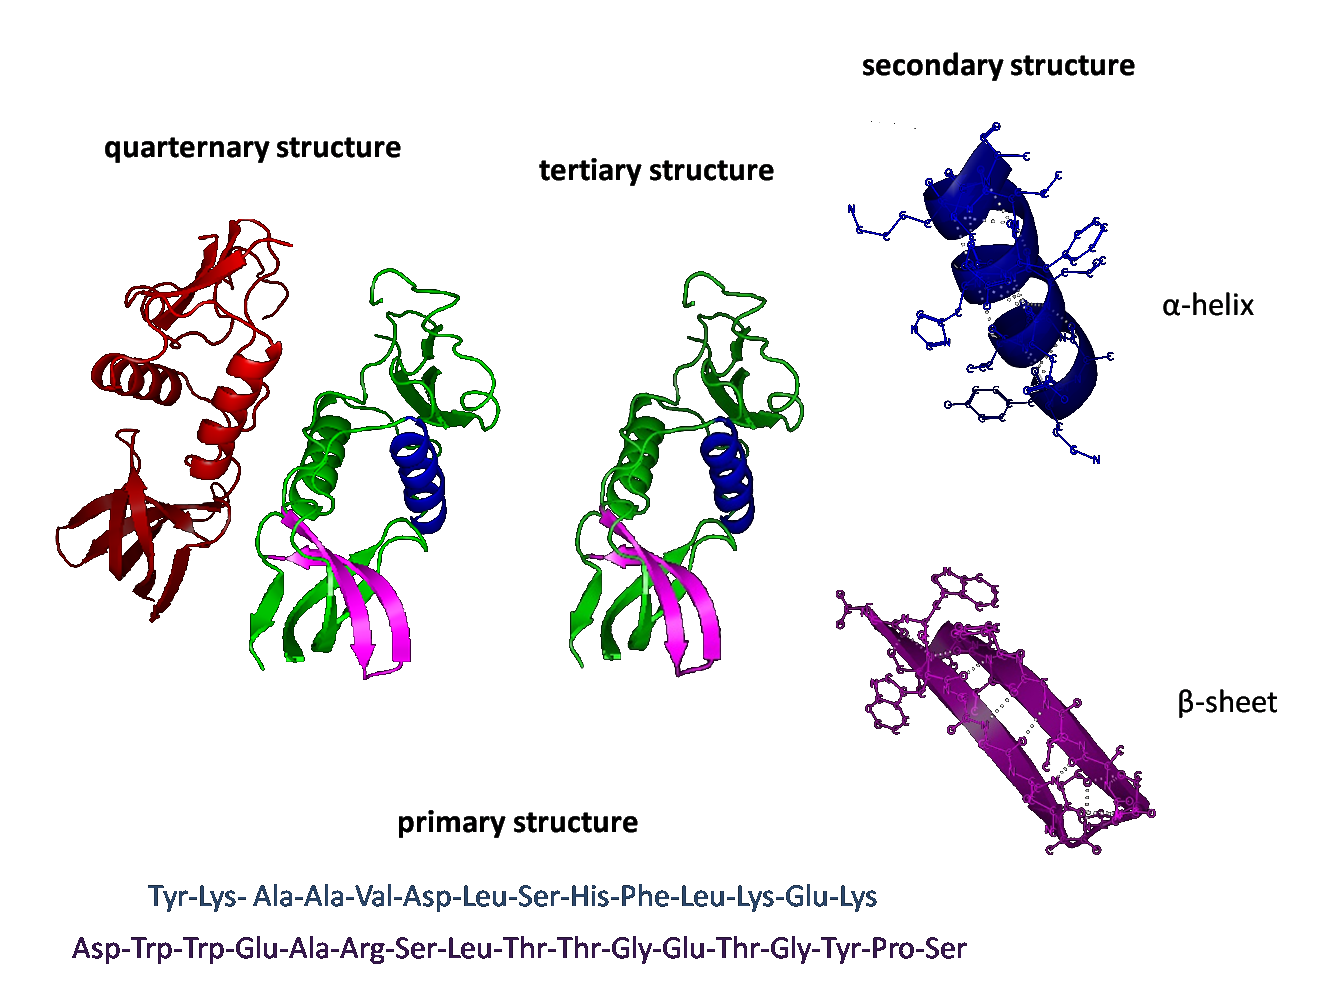
\includegraphics[width=21cm]{figures/Protein_structure}
\caption[Structure levels of the protein 1EFN]{Structure levels of the protein 1EFN. Adapted from \emph{Wikipedia}}
\label{fig:Protein_structure}
\end{center}
\end{figure}
\end{landscape}


%*****************************************************************************
%\begin{itemize}
%\item Popis řešeného problému, vymezení cílů DP/BP a požadavků na implementovaný systém.
%\item Popis struktury DP/BP ve vztahu k vytyčeným cílům.
%\item Rešeršní zpracování existujících implementací, pokud jsou známy.
%\end{itemize}

%*****************************************************************************
\chapter{Solution design}
\label{ch:sol}
% Analýza a návrh implementace (včetně diskuse různých alternativ a volby implementačního prostředí).

\section{Data sources and preprocessing}
\label{sec:data}
In this section, the nature and sources of the input data used later for machine learning are described.

\subsection{Gene Ontology}
\label{ssec:go}
Gene Ontology (GO) \cite{go} is a representation of relationships among various \emph{terms} identifying common (species-independent)
biological processes, cellular components and molecular functions.
The GO terms definitions and relationships among them are provided by human experts. 
In this work, we are only interested in terms identifying molecular functions and the $is\_a$ generality relation among them
(denoted here by the symbol $\prec$).
These terms together with the $\prec$ relation form a directed acyclic graph.
There is a special node called simply ``molecular function'',
which is the most general term and represents arbitrary protein function;
it has zero outgoing edges in the graph.
The GO terms themselves are unambiguously identified either by a numerical id (e.g. GO:0046872) or a human-readable name
(``metal ion binding'', in this case).
The $\prec$ relationship maps a term to more general ones. So for example GO:0046872 $\prec$ GO:0043169 (``cation binding'')
 and GO:0043169  $\prec$ GO:0043167 (``ion binding'').
 The $\prec$ relation is implicitly transitive,
 thus for for example also ``metal ion binding''  $\prec$ ``ion binding''.
 
The core ontology used in this thesis is the \texttt{go-basic.obo} \cite{gores} \url{http://geneontology.org/page/download-ontology} provided by the Gene Ontology Consortium. 
It serves two purposes in this work:
1) In the initial steps of the work, it is a simple list of protein functions.
The molecular function terms are the protein functions studied in this work.
In this context, general functions are studied alongside specific ones. 
2) The underlying directed acyclic graph is used as the skeleton for construction of the 
Bayesian network in the consistency correction step. 

There are over 10~000 terms in the ``molecular function'' namespace of Gene Ontology.
A~certain subset has to be selected for two reasons:
1) Most terms are too specific and have currently very few (or even none at all) proteins associated with them
and therefore are useless for machine learning.
2) The performed computations are difficult and computationally costly.
Therefore only the terms which have the most proteins associated with them are used.
Due to the transitivity of the $\prec$ relation,
these also happen to be some of the most general terms in the core ontology.
The used subset of the ontology is displayed on Figure \ref{fig:go}.
                                                                                                                                                                                                                                                                                                                                                                                                                                                                                                                                                                                                                                                                                                                                               

\subsection{Proteins}
\label{ssec:proteins}
Data about proteins used in this work were extracted from Research Collaboratory for Structural Bioinformatics (RCSB) Protein Data Bank (PDB) \cite{pdb}.
PDB currently publishes over 100~000 entries containing information about identified existing protein structures.
The entries contain various details about the protein,
but only the protein identifier and structure are used in this work.
The following data are thus extracted from each used entry:
\begin{itemize}
 \item Protein name -- identifier. If a protein has a quaternary structure,
 it is separated into polypeptide strands each of which has a unique identifier and associated GO terms
 (possibly distinct terms among strands of the same complex.)
 \item Primary structure -- the linear chain of amino acid residues.
 Many proteins in PDB have unidentified terminating (or sometimes other) amino acid residues.
 Only proteins with more than 90\% of it's primary structure identified are used.
 The relational representation of proteins offers a simple way of dealing with missing amino
 acid residue information, as we will see later in subsection \ref{ssec:relrepr}.
 \item Secondary structure -- the information describing to which type of secondary structure each amino acid residue belongs.
 It could be of unknown/unidentified type. In an average PDB protein entry containing secondary structure information, 76\% of residues have an associated secondary structure.
 Only proteins with at least some information about secondary structure are used.
 \item Tertiary structure -- PDB contains detailed data about positions of various atoms in each amino acid residue.
 This information cannot be used in completeness for tractability reasons. 
 Only the coordinates of the $\alpha$-carbon on each amino acid residue are used in computations.
 Before the relational learning phase, coordinates are used to calculate distances between $\alpha$-carbons discretized to 2Å.
 Notice, however, that PDB entries often have resolution worse than 2Å.
 This is a potential problem in the data.
 The rationale behind including entries with worse resolution is that the data set will be large and thus the solution
 is expected to be robust towards these atom position measurement errors.
\end{itemize}

Another information that PDB provides and could be used in learning is the ligand information.
(\emph{Ligand} is the active site of the protein, for example a binding site.) 
The idea is that protein function is mostly determined by the ligand and
that the structural parts distant from the ligand are not so important.
If only information about residues with certain distance from ligands were used,
the data set size could be greatly reduced possibly bearing almost the same information
exploitable for learning.
Hence, it would be feasible to learn from larger data set and train a better classifier.
Application of this idea was rejected in this work,
because it is unclear how much is ligand information defining for each GO term (protein function)
or how large ligand neighbourhood is suitable,
but it is reasonable to assume that it varies. 
Therefore the evaluation results would be biased and performance results of prediction
on different protein functions could not be compared.
It is, however, an interesting problem for future research in this field.

\paragraph{Data location} Local mirrors of PDB databases were used in this work (see \url{http://www.rcsb.org/pdb/static.do?p=download/ftp/index.html}.)
Secondary structures in FASTA format are available from \url{http://www.rcsb.org/pdb/static.do?p=download/http/index.html}.)
Protein annotations, i.e. data that associate GO terms with actual genes (proteins -- PDB entries), were downloaded from
\url{http://geneontology.org/page/download-annotations}, 
the file \url{http://geneontology.org/gene-associations/gene_association.goa_pdb.gz}.
Proteins, that are not associated with any of the studied functions are discarded from the data set.

\paragraph{Species} The association file also contain information about the biological taxon from which the protein was taken.
In this work only proteins from \emph{Homo sapiens} were used.
(UniProt taxon id 9609 identifies \emph{Homo sapiens} in the association file.) 
The assumption behind this is that learning on a single organism should result in
greater prediction precision for that organism.
With relational learning methods however, it would be interesting to study, if there exist protein
structural patterns for a given function, that are common even in evolutionary distant species.

\paragraph{Protein confomations}
In the work \cite{szabova} where similar methods were used to predict DNA-binding protein 
function, only proteins in either their bound or unbound confomation were used.
Arranging the data set to include only proteins of specific type of
confomation makes sense if: 1) It is easy to determine this confomation type 
before presenting a yet unidentified protein to the classifier. 
2) This specific confomation is defined for the studied function.
For binding proteins, this confomation type is either the bound
or unbound confomation.
In this work, the confomation is not taken into account, though.
First, it is not obvious how to define the right confomation
type for each function, since also non-binding functions
are studied here (for example catalytic activity).
Although binding proteins form a large subset of all the proteins
in the dataset, using only (un)bound confomations  for them  would introduce
some bias in the comparison of classification results.
An advantage of not using specific confomation is that 
the classifier should then learn to recognize 
the protein in any confomation.
(Albeit possibly with lesser precision.) 

\subsection{Non-redundant data set}
\label{ssec:redundancy}
One problem with Protein Data Bank is that it contains many redundant entries --
proteins that are almost identical.
That can be caused for example by 
including a certain protein and also a protein that differs 
only by a minor mutation which can even preserve the protein's function.
Redundant entries should be removed from the data being used for machine learning for two reasons:
1) They bloat the data set making the learning more computationally difficult.
2) As a consequence of redundancy, many similar entries could appear in both training and testing data set
which would yield overly optimistic results when evaluated, 
while the classifier could actually be overfitted.
It is not obvious, how redundancy or protein similarity should exactly be defined,
but in this work the approach to redundancy and it's removal described by \cite{maxind} is loosely followed.

The basic idea is the following: 
Assume, that there exists a reasonable similarity relation on the protein data set. 
This relation is represented by a graph -- distinct proteins are nodes and there
is an edge between each two proteins that are similar according to the given relation.
We define a non-redundant data set to be a set of proteins such that no two are similar.
In other words, we would like to find a set of nodes in that graph such that no two are adjacent
and we prefer this set to be the largest possible.
This is a non-formal definition of the maximum independent set problem in graph theory.
It is known to be NP-HARD, but fortunately a heuristic solution suffices.
The following simple heuristic is employed:
Start with empty independent set.
Until no more nodes can be added to the independent set,
iteratively pick a random node from the graph,
put it to the independent set and remove all adjacent nodes from the graph.
Repeat the whole process several times and select the best solution (largest independent set).

Now, the similarity of two proteins is defined as the inverse of their local alignment \emph{E value} computed by BLAST \cite{blast} \cite{blastp}.
BLAST is an algorithm that finds and measures local alignment of two sequences,
in our case of the sequences of amino acid residues of two proteins. 
This means, it is a distance measure based purely on the primary structure of proteins.
Let us denote by $S = BLAST(A,B)$ the score of alignment 
of two proteins $A, B$. (Where BLOSUM62 substitution matrix is used.) 
The BLAST program then also computes a number called \emph{Expect value} or simply \emph{E value}, 
defined as follows:
\[ E = K \cdot l_A \cdot l_B \cdot e^{-\lambda \cdot S}, \]
where $l_A$ and $l_B$ are lengths of the sequences $A,B$ respectively and $K$ and $\lambda$ are constant parameters.
The E value can be interpreted as the expected number of proteins present in a database of a given size
that would have an alignment witch score $S$ or higher simply by chance.
Here, the E value is used in the following way: We define that $A$ is similar to $B$ if $E < T$ for some threshold $T$.
Note, that generally $BLAST(A,B) \neq BLAST(B,A)$,
so the closure under symmetry for the similarity relation is actually used.
The question remains, how to choose the value $T$.
For the purpose of this work, $T = 10^{-50}$ was used.
This choice was made intuitively and ad-hoc (to keep the data set large enough, see below),
since the author is not aware of any theory that would guide such decision.
But at least to illustrate what the value means, here is an example of best local alignment match
for two variants of the lysozyme protein (PDB ids 132L and 1QSW), for which the \texttt{blastp} program computed E value of $10^{-50}$
(i.e. no proteins that would be ``more similar'' appear in the data set together.):
\begin{minipage}{\linewidth}
\begin{verbatim}


132L: KVFGRCELAAAMKRHGLDNYRGYSLGNWVCAAKFESNFNTQATNRNT-DGSTDYGILQINSRWWCNDGRTP
Match KVF RCELA  +KR G+D YRG SL NW+C AK+ES +NT+ATN N  D STDYGI QINSR+  NDG+TP
1QSW: KVFERCELARTLKRLGMDGYRGISLANWMCLAKWESGYNTRATNYNAGDRSTDYGIFQINSRYCANDGKTP
      GSRNLCNIPCSALLSSDITASVNCAKKIVSDGNGMNAWVAWRNRCKGTDVQAWIRGCRL
      G+ N C++ CSALL  +I  +V CAK++V D  G+ AWVAWRNRC+  DV+ +++GC
      GAVNACHLSCSALLQDNIADAVACAKRVVRDPQGIRAWVAWRNRCQNRDVRQYVQGCGV
      
      
\end{verbatim}
\end{minipage}
Here, amino-acid residues are encoded by the standard single-letter code (see table \ref{tab:aaprops} for reference). 

Some disadvantages follow from using BLAST as distance function.
There could be some proteins which have the same primary structure, 
but can exist in varying spatial conformation exhibiting different functions.
It would do no harm to include both in the data set if the difference is large enough.
For BLAST, however, they will be indistinguishable and as a~result 
only one of them will appear in the final data set.

\section{Relational learning}
In this section, approach to machine learning using relational learning based on structural patterns
is briefly explained and 
it's application to the protein function prediction in this work is explained.

\subsection{Relational representation of proteins}
\label{ssec:relrepr}
Let us first define how proteins can be represented as first order logic propositions.
The data are going to be fed to the RelF algorithm,
which expects a set of conjunctions of positive ground literals.
The representation should therefore respect this limitation.

Relational representation of data is naturally discrete.
The basic discrete unit of protein is a single amino acid residue,
so our relational description of a protein consists mainly
of literals describing that there is a certain relationship between 
two residues or that a residue has a certain property.
(In theory, it could be more than two, but that is not used here.)
Further, discretized information about polarity and electrical charge
is encoded in the rest of each conjunction as \emph{background knowledge}.

Let us start with a simple step-by-step example illustrating how information about
peptide primary structure could be encoded.
Assume for example a peptide Glu-Pro-Asp, a subsequence of the protein 1APJ.
First, let us encode the simple fact,
that there are three distinct residues, as the following conjunction:
\[ Res(r1) \land Res(r2) \land Res(r3). \]
Now we can add the information about the residue type. The conjunction becomes:
\[ Res(r1) \land Type(r1, glu) \land Res(r2) \land Type(r2, pro) \land Res(r3) \land Type(r3, asp). \]
This still contains no information about the primary structure, 
which could be inserted in the following way:
\begin{align*}
Res(r1)& \land Type(r1, glu) \land \\
Res(r2)& \land Type(r2, pro) \land Next(r1, r2) \land \\
Res(r3)& \land Type(r3, asp) \land Next(r2, r3). 
\end{align*}
The predicate $Res$ may seem redundant now.
The reason why it is included is that it makes it algorithmically easier to deal with incomplete information about a residue.
We may not know the residue type, but perhaps we know some other information about it, for example the $Next$ relation in this case.
It is also exploited in templates for the RelF algorithm later.

\pagebreak
The following information is actually encoded in the implementation of this work:
\begin{itemize}
 \item Residue type -- simply the type of each amino acid, if it is known.
 \item Distance between residues -- distances of $\alpha$-carbons discretized to 2Å with upper bound 14Å.
 This is a tertiary structure information, but it also implicitly includes primary structure 
 as neighbouring amino acid residues are never much distant.
 \item Secondary structure type of which the residue is part.
 \item Background information -- polarity (polar / nonpolar) and electrical charge (positive / neutral / negative)
 information about amino acids.
 No information about amino acids outside this background knowledge is used.
\end{itemize}

The Glu-Pro-Asp subsequence of 1APJ from the example is then encoded in the following way:
\begin{align*}
&Res(r1) \land Type(r1, glu) \land SecStr(r1, turn) \land \\
&Res(r2) \land Type(r2, pro) \land SecStr(r2, turn) \land Dist(r1, r2, 8) \\
&Res(r3) \land Type(r3, asp) \land SecStr(r3, bend) \land Dist(r2, r3, 8) \\
&Polarity(glu, polar) \land Charge(glu, negative) \land \\
&Polarity(pro, nonpolar) \land Charge(pro, neutral) \land \\
&Polarity(asp, polar) \land Charge(asp, negative).
\end{align*}

Notice, that we can also think of the conjunction as a certain first order logic interpretation:
it defines for which tuples of constants the used predicates are true.
Each protein in the data set is converted to this relational form.
It is obvious that this representation of proteins is great simplification.
The hope is that this model captures some of the essential properties of the 
protein while it is computationally feasible to work with such model.

Also notice, how easy it is in this relational representation to deal with missing data:
If for example we do not know the secondary structure in which a certain amino acid 
residue occurs or the polarity of an amino acid in case of Asx and Glx (see Table \ref{tab:aaprops})
or even if there is completely missing information about an amino acid residue,
we can simply omit the literals relevant to this information.
So for example if we did not know the secondary structure of $r1$,
we would drop the literal $SecStr(r1, turn)$ in the above example.
However, this is not completely correct approach and it introduces noise in the data:
The algorithms that later work with this data cannot distinguish information
that is not known and information that is know to be false.
For example,
not including $SecStr(r1, turn)$ because we do not know it although it is true
is very different from not including $Type(r1, ala)$ which is know to be false.
Yet, these two cases are represented the same way.

The used charge and polarity properties of amino acids (the background knowledge) are displayed in table \ref{tab:aaprops}.
\begin{table}
\begin{center}
 \begin{tabular}{lccrr}
\textbf{Name} & \textbf{Code} & \textbf{Abbreviation} & \textbf{Charge} & \textbf{Polarity} \\
\hline
Alanine & A & Ala & neutral & nonpolar  \\ \hline
Arginine & R & Arg & positive & polar  \\ \hline
Asparagine & N & Asn & neutral & polar \\ \hline 
Aspartic acid & D & Asp & negative & polar  \\ \hline
Asparagine or aspartic acid & B & Asx & ? & polar \\ \hline 
Cysteine & C & Cys & neutral & nonpolar  \\ \hline
Glutamine & Q & Gln & neutral & polar  \\ \hline
Glutamic acid & E & Glu & negative & polar \\ \hline
Glutamic acid or glutamine & Z & Glx & ? & polar \\ \hline
Glycine & G & Gly & neutral & nonpolar \\ \hline
Histidine & H & His & neutral & polar \\ \hline
Isoleucine & I & Ile & neutral & nonpolar \\ \hline
Leucine & L & Leu & neutral & nonpolar \\ \hline
Lysine & K & Lys & positive & polar \\ \hline
Methionine & M & Met & neutral & nonpolar  \\ \hline
Phenylalanine & F & Phe & neutral & nonpolar  \\ \hline
Proline & P & Pro & neutral & nonpolar \\ \hline
Pyrrolysine & O & Pyl  & neutral & polar  \\ \hline
Selenocysteine & U & Sec & negative & polar  \\ \hline
Serine & S & Ser & neutral & polar  \\ \hline
Threonine & T & Thr & neutral & polar \\ \hline
Tryptophan & W & Trp & neutral & nonpolar   \\ \hline
Tyrosine & Y & Tyr & neutral & polar  \\ \hline
Valine & V & Val & neutral & nonpolar \\ \hline
Leucine or islueucine & J & Xle & neutral & nonpolar \\ \hline
Unknown or unidentified & X & Xxx & ? & ? \\ \hline
\end{tabular}
\caption[Proteinogenic amino acids and their used properties]{Proteinogenic amino acids and their used properties.
The data were copied from TreeLiker software example files.}
\label{tab:aaprops}
\end{center}
\end{table}


\subsection{Learning with relational features}
A technique called \emph{propositionalization} is employed in this work. 
Generally, propositionalization is the transformation of a relational data set
into an attribute-value data set.
Attribute-value data set can then be used as input to many
state of the art machine learning algorithms, such as 
Support Vector Machines.
In this work, we use the RelF algorithm to perform the propositionalization,
but in principle different supervised propositionalization
techniques could be examined in this context.
The TreeLiker software (\url{http://ida.felk.cvut.cz/treeliker/TreeLiker.html})
was used as the implementation of RelF here.

A brief description of the propositionalization idea used in RelF algorithm follows.
For more detailed description, see the article \cite{relf}.
A broader view on propositionalization and the topic learning relational features is in \cite{kuzelka}.
RelF could be classified as an inductive logic programming (ILP) algorithm.
There are two important notions -- \emph{$\theta$-subsumption} and \emph{$\theta$-reduction} --
in many ILP problems including the RelF propositionalization technique.
Further, the notion of \emph{tree-like} conjunction property is needed 
for understanding of the propositionalization results.
So let us first remind their definitions (adapted from \cite{szabova},\cite{relf}): 

\paragraph{Definition} ($\theta$-subsumption) Let $A,B$ be clauses. 
The clause $A$ \emph{$\theta$-subsumes} $B$ (written $A \preceq_{\theta} B$)
iff there exists a substitution $\theta$ such that $ A \theta \subseteq B$.
If $A \preceq_{\theta} B$ and $B \preceq_{\theta} A$, we call $A$ and $B$ 
$\theta$-equivalent (written $A \approx_{\theta} B$).

\paragraph{ } The motivation for the definition of $\theta$-subsumption is that it is a decidable
(but incomplete) approximation of the covering (semantic consequence, $\vDash$) relation,
which itself is undecidable in general.
To be precise, if $A \preceq_{\theta} B$ then $A \vDash B$. \cite{plotkin}

\paragraph{Definition} ($\theta$-reduction) Let $A$ be a clause.
If there exists a $R$, such that $|R| < |A|$ and $A \approx_{\theta} R$,
we say that $A$ is \emph{$\theta$-reducible}. 
A minimal such $R$ is called the \emph{$\theta$-reduction} of $A$.

\paragraph{Definition}   (Tree-like conjunction) A first-order logic conjunction (hypergraph) $C$
is said to be \emph{tree-like} if the iteration of the following rules on $C$
produces the empty conjunction:
\begin{enumerate}
 \item Remove an atom (hyperedge) which contains fewer than 2 terms (nodes).
 \item Remove a term (node) which is contained in at most one atom (hyperedge).
\end{enumerate}


\paragraph{ } The basic idea in RelF propositionalization technique is now presented.
RelF takes as input a relational data set
where each member is labeled as belonging to either positive or negative class
and a \emph{template}. 

The data set is a set of first order logic conjunctions with positive ground literals,
or equivalently set of first order logic interpretations.
Transitivity of the $\prec$ relation is assumed for labeling the data.

The template is a definition of a set of conjunctions called \emph{features}
(notice: not anymore with all terms ground)
that have the tree-like property. 
The template itself is a conjunction,
but the arguments of literals are \emph{variable types} and each of them has an associated \emph{mode}.
The type can be arbitrary and the mode can be one of:
input (marked by a +), output (marked -) or constant (marked \#).
An example of a template is:
\[ Res(-a)\land Res(+b)\land Dist(+a, -b, \#n)\land Type(+b, \#t)\land Type(+b, -s)\land Polarity(+s, \#p). \]
By definition, for a given variable type, there has to be exactly one instance of it 
marked as output and at least one marked as input in the template.
Further the following graph constructed from the template must not contain oriented cycles: 
In the graph, there is a node for each variable type in the template and an edge $a \rightarrow b$
iff there is a literal which contains $+a$ and $-b$.
These conditions ensure,
that the generated features have the tree-like property.
Observe, that both these conditions hold for the example.
Features can be generated from the template by the following procedure:
\begin{enumerate}
 \item Start with empty conjunction.
 \item Select a literal from the template, that does not have any of it's arguments marked as input.
 \item Add the literal(s) to the conjunction replacing the input and output type variables by variables.
       (For input type variables, if a variable was assigned to it previously in the run of the algorithm,
       it will be used. Otherwise a new variable is generated.)
       Constant type variables are replaced by some constant values of appropriate type.
 \item Select other literals from the template where the type variables from the previous step are marked as output.
 \item Repeat steps 3-4 until there are no more type variables.
 \item One feature is completed, another one can be generated by keeping the conjunction and jumping to step 2.
\end{enumerate}
Only $\theta$-irreducible features are outputted. 
Note, that the actual implementation is different with regard to redundancy filtering. 
It is proven in \cite{relf} that there is only a finite number of $\theta$-irreducible tree-like features
which can be generated this way.
An example of a feature that can be generated by RelF using the template from the example is:
\[ Res(A) \land Res(B)\land Dist(A,B,8)\land Type(A, lys)\land Type(B, T)\land Polarity(T, polar). \]
Due to the possibility to repeat the procedure from step 6,
more residues could be added to the feature and we can have for example a feature like:
\[ Res(A)\land Res(B)\land Res(C)\land Dist(A,B,8)\land Dist(A,C,10). \]
But not:
\[ Res(A)\land Res(B)\land Res(C)\land Dist(A,B,8)\land Dist(\mathbf{B},C,10). \]
A comprehensive, more detailed discussion on templates and their usage in the TreeLiker software
can be found in \cite{szabova}.

With this input, RelF examines the $\theta$-irreducible features that it generates from
the template and evaluates if they are covered (in the sense of $\theta$-subsumption)
by some of the examples in the data set.
If yes, it stores this feature and outputs it's evaluation,
which can be either binary (is covered / is not)
or numerical (the number of different grounding substitutions $\theta$ 
such that $F \preceq_{\theta} E$ for the feature $F$ and example $E$.)
Furthermore, redundant features are discarded.
The precise definition of redundancy \cite{relf} is somewhat complicated,
but it basically says that a feature $F$ is redundant (w.r.t. positive, resp. negative class)
if there exists a different feature $F'$ such that $F$ and $F'$ cover
the same negative (resp. positive) examples but $F$ covers only a subset
of positive (resp. negative) features covered by $F'$.
The purpose of limiting the set of possible features to only \emph{tree-like}
is the problem's tractability.
In general,
the $\theta$-subsumption and $\theta$-reduction problems are NP-HARD.
For propositions which are tree-like, however, the $\theta$-subsumption and $\theta$-reduction subproblems 
(which obviously have to be solved many times during the RelF algorithm run)
can be solved in polynomial time, which makes the task tractable.

The results in \cite{szabova} show,
that it is a significant advantage to use the RelF variant with grounding counting
for DNA-binding protein function prediction.
This is because features here correspond to protein structural patterns and
it is not surprising that if a structural pattern know to be determining a certain function
appears more frequently in a protein, it is more likely to exhibit that function.
Also notice, that binary output would not provide any advantage when further piped to Support Vector Machines algorithm.
Therefore, the grounding counting RelF variant is also applied in this work. 

After the propositionalization process is finished for a given function,
the outputs are used to train a classifier
such as Suppor Vector Machines (SVM), Random Forest or \mbox{AdaBoost}.
With regard to the next step of consistency correction,
the nature of the classifier decision function has to be considered.
SVMs have a continuous decision function
(oriented distance from the separating hyperplane)
and the distribution of it's values on testing data could be 
roughly approximated by a mixture of two normal distribution (one for positive and one for negative examples).
The distance of their means is then a measure of class separability.
For the later two classifier types the decision function
would be discrete (votes of the sub-classifiers in the ensemble)
and it's distribution on testing data could perhaps be approximated by a mixture of two binomial distributions.
Only SVMs were used in this work, though.

The propositionalization process is performed for each studied function,
where negative examples are taken from the set of proteins which are not annotated
as having the function.
This may not be always true.
It is reasonable to expect that the laboratory protein
function identification processes do not misidentify the protein as having a function that it actually does not have.
However, it is not realistic to assume that it will always identify all of the functions
the protein has. 
This way a protein with a certain function could end up appearing as a negative example 
for that function, simply because that function has not yet been identified.
This suggests that perhaps semi-supervised learning should be used instead.
However, there are several problems with that.
In regard to RelF, this would require alterations in the definition of redundancy which 
could have significant impact on the algorithm.
Dropping the redundant features filtering would cause a decrease in performance
of uncertain extent. 
The author of this work is not aware of any theory, that would describe such situations.
Further, it is not obvious how to label at least some of the negative examples --
i.e. to to find a subset of the data set that certainly does not have the studied function.
Semi-supervised learning algorithms Label Propagation and Label Spreading \cite{semi}
where briefly examined as a replacement for SVM.
RelF ran on fully labeled data set as described above, but semi-supervised learning
ran with positive examples labeled only.
The resulting classifiers were only slightly better than ``random classifier''
and hence far inferior to SVM (details on SVM performance are discussed in chapter \ref{ch:results}).

The complete template used here as input to RelF is the following:
\begin{align*}
&Res(-a) \land Res(+b) \land Dist(+a,-b, \#num) \land  \\
&Type(+a, \#rt) \land Type(+b, \#rt) \land \\
&Type(+a, -r1) \land Type(+b, -r2) \land \\
&Charge(+r1, \#chrg) \land Charge(+r2, \#chrg) \land \\
&Polarity(+r1, \#pol) \land Polarity(+r2, \#pol) \land \\
&SecStr(+a, \#s) \land SecStr(+b, \#s).
\end{align*}

\section{Proposed consistency correction}
As mentioned earlier, one issue with the prediction is that is does not have to be
consistent with respect to the Gene Ontology.
The trained SVMs may, for example, classify a certain protein
as \emph{metal ion binding}
but not \emph{ion binding}.
Such result is difficult to interpret;
without further knowledge we cannot decide
which of these two functions the protein actually has.

A naive solution could be for example
to consider only the most specific terms
for which the classifier outputted \emph{yes}
and by the transitivity of the ontology also
classify all of the more general terms as \emph{yes}.
However, this approach ignores the information
provided by the classification output on these
general terms. 

A method described in \cite{bnet} is designed
as an alternative solution which exploits this
information to make the classification more precise.
The idea is to construct a Bayesian network based on
the used ontology.
The knowledge that helps us decide the function
in case of inconsistency
is hidden in the parameters of the probability 
distributions in it's nodes 
which can be learned from relationships between
labels on both training and testing data.
In the experimental settings of \cite{bnet},
this solution not only made the classification 
consistent,
but it also improved it for most (but not all) nodes.
That is the major reason, why it is also tested in this work.

The basic structure of the network is the same as the used ontology 
with the $\prec$ relation. 
Nodes in this structure standing for molecular functions
in the ontology are called \emph{hidden nodes} (marked $y_i$ in Figure \ref{fig:net}). 
The direction of the nodes is unchanged.
This intuitively makes sense,
because the direction of arrow in a Bayesian 
network should mean causation
and a we can think of a more specific term as partial cause
for a more general one but not the other way around.
Further note, that relationships which are implied by the implicit transitivity
of $\prec$ relation are not included -- only direct child to parent connections are.
Finally, each hidden node has exactly one extra child node, these
are called the \emph{observed nodes} (marked $\hat{y}_i$ in Figure \ref{fig:net}).
The intended use of this network
is marking all of the \emph{observed nodes} as observed
while assigning them value of the output 
of the classifier of their respective function from the previous step.
It can be a real number -- the output of the classifier's decision function,
or simply a binary value representing the classifier's decision.
Then an inference algorithm is ran
to find the most likely consistent assignment of binary (yes / no) values to be assigned to $y_i$
and these inferred values in the hidden nodes 
are thresholded to produce the final classification output.


\begin{figure}[h]
\begin{center}
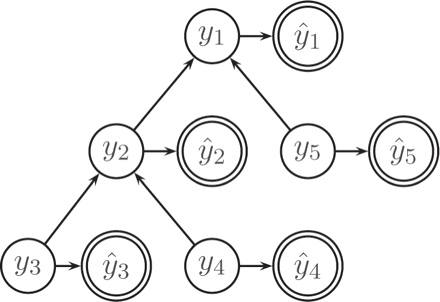
\includegraphics[width=5.5cm]{figures/net}
\caption[Example of the structure of the Bayesian network]{Simple example of the structure of the network.
Figure copied from \cite{bnet}.}
\label{fig:net}
\end{center}
\end{figure}

More formally, we want to find such consistent $y_1, ..., y_n \in \langle 0, 1 \rangle$
(where $n$ is the number of nodes in the network)
which maximize the expression:
\[P(y_1, ..., y_n \,|\, \hat{y}_1, ..., \hat{y}_n) \propto P(\hat{y}_1, ..., \hat{y}_n\, | \, y_1, ..., y_n) \cdot P(y_1, ..., y_n). \]
Since the variables $\hat{y}_1, ..., \hat{y}_n$ are independent (classifiers do not communicate), we can factor the conditional probability:
\[P(\hat{y}_1, ..., \hat{y}_n\, |\, y_1, ..., y_n) = \prod_{i=1}^n P(\hat{y}_i \,|\,y_i). \]
Notice, that $\hat{y}_i$ is real number,
we will assume the distribution of $P(\hat{y}_i\,|\,y_i)$ to be Gaussian.

% TODO FIXME zdůvodnění proč je Gaussian
%Then the joint distribution $P(\hat{y}_i, y_i)$ would be a mixture of Gaussians
%with the mixture coefficients being the probabilities $P(y_i)$.
Provided the network structure, using the conditional independence rule,
the joint probability on $y_i$ can be factored as:
\[ P(y_1, ..., y_n) = \prod_{i=1}^n P(y_i\,|\,\{y_j : j  \,  \prec \,  i\}). \]

Now, conditional probability tables for the distributions $P(y_i\,|\,\{y_j : j  \,  \prec \,  i\})$ 
can be simply computed from \emph{training} data by counting occurrences.
A prior count of 1 sample for each case is used to avoid the 
possibility of zero probability for some cases.
To ensure consistency of the output, however, 
we shall set:
\[ P(y_i = \top \, | \, \exists y \in \{y_j : j  \,  \prec \,  i\}, \, y = \top  ) = 1, \]
which means that a node must be positive if some more specific term is positive.
And in fact, we again use a value close to 1 such as 0.99 in place of 1 to avoid zero probability for the other case causing problems during inference.
The parameters of the probabilities $P(\hat{y}_i\,|\,y_i)$ can be
calculated by taking part of the \emph{testing} data
(not used later for evaluation) to
obtain some number of $y_i, \hat{y}_i$ value pairs and estimate the parameters of $P(\hat{y}_i\,|\,y_i)$ from them,
for example by the maximum likelihood method.
In case of a binary classifier, 
these parameters are contained within the confusion matrix divided 
by the number of tested samples.

There is one exception to the above: 
The most general function called ``molecular function'',
which is true for any protein
(and thus it does not even make sense to train it.)
We set the conditional probability table trivially to:
\[ P(molecular\_function = \top \,|\, anything ) = 1. \]

This assumption that the distributions of $P(\hat{y}_i\,|\,y_i)$ are Gaussian  
deserves some justification.
It is an ad-hoc assumption:
Some simple distribution is needed to for us
to be able to perform Bayesian inference
and using a continuous distribution,
already makes inference somewhat difficult.
See the Figure \ref{fig:gaussians}
for sample comparison with experimental results.
We can see that the real underlying distributions are apparently not exactly Gaussian,
but close enough to be reasonably approximated as Gaussian.
It could be examined by statistical normality tests to get more detailed view on this assumption.

\begin{figure}[h]
\begin{center}
\includegraphics[width=12cm]{figures/g}
\caption[Probability distributions of decision function values for DNA binding]{Distributions of decision function values for DNA binding protein function -- histograms of real data and estimated Gaussians;
horizontal axis shows the oriented distance from the SVM's separating hyperplane, vertical axis shows probability density.
The ratio of occurrences in data set is not taken into account in this plot.}
\label{fig:gaussians}
\end{center}
\end{figure}

Inference on this Bayesian network is done using the \emph{variational Bayes} \cite{varb} method.
Variational Bayes is an algorithm used to
obtain the approximate posterior probabilities $P(y_i \, | \, \hat{y}_1, ..., \hat{y}_n).$
It was chosen, because it can handle nodes with Gaussian distributions within the network.
Once we have the posterior probabilities, 
we can simply make the final classification by setting:
\[ y_i := P(y_i = \top \, | \, \hat{y}_1, ..., \hat{y}_n) > \frac{1}{2} \, \, \forall i. \]

\section{Experimental settings and methodological remarks}
\label{sec:method}
In this section, the experimental setting confomation and
methodology concerning the evaluation
of the experimental results are discussed.

With the filtering described in subsection \ref{ssec:proteins}
and making the dataset non-redundant as described in subsection \ref{ssec:redundancy},
we ended up with 3607 proteins.
This number is reduced to $2^{11} = 2048$ for tractability (but also aesthetical) reasons. 
That is still significantly more than the size of the largest data set used in the work
\cite{szabova} for DNA binding prediction,
where 138 DNA-binding and 843 non-DNA-binding (981 in total) proteins were used.

The same set is used for all studied functions.
Given this set, only functions from the Gene Ontology that have at least $2^7 = 128$
proteins associated with them (considering transitivity of $\prec$) are used.
The resulting subset of the ontology with it's structure is displayed on Figure \ref{fig:go}.
The GO identifiers and the numbers samples for each of there function is present in Table \ref{table:terms}.  
TreeLiker is then configured to run with subsampling.
That means, that RelF is ran repeatedly on a random subset of the whole data set
and in the end, it outputs the data propositionalized on the
union of features found in all iterations.
Sample size is set to $2^9=512$ and number of samples (iterations) is set to $2^3=8$.


\begin{landscape}

\begin{figure}[h]
\begin{center}
\begin{tiny}
\includegraphics[width=22.5cm]{figures/go.tikz}
\end{tiny}
%\includegraphics[width=22cm]{figures/go-basic_children}
\caption{The used subset of the Gene Ontology}
\label{fig:go}
\end{center}
\end{figure}
\end{landscape}

The following method is used to process data:
Using 8-fold cross-validation split the input proteins into folds
containing training and testing data.
RelF is ran on training data and the testing 
data are propositionalized given the features learned by RelF.
Testing data in each fold are further split into two equally sized parts,
let us call them ``test'' and ``validation'' sets.
The size of both test and validation set is thus $2048 / 8 / 2 =  128$.
Classifiers are fitted on the propositionalized training data.
The state of the art SVM classifier with Radial Basis Function (RBF)
kernel and $C = 1$ parameter is used.
Random forest and AdaBoost classifiers were also examined 
and they tend to give similar results as RBF SVM,
but the nature of their decision function is different
and would require appropriate modifications in the construction of the 
correcting Bayesian network.
Since SVM require the features to be comparable,
the individual features are scaled to zero mean and unit variance.
(Testing data are scaled the same way as training data.)
Then, the training samples are weighted in such way, that the total weights
of positive samples are equal to the total weight of negative samples.
Samples within each class have equal weights. 
(This could be refined for example by assigning lesser weight
to proteins with more unknown information.)
Subsequently the correcting Bayesian network is constructed
for each fold by taking classifiers of all functions trained
on the train set in the given fold
and the probabilities $P(\hat{y}_i\,|\,y_i)$ are estimated from the test set.
The performance of the classification both before and after the correction
is performed on the validation set.

% TODO: Výpočet jak moc vadí ne-stratifikace
This approach is not perfect. 
A noteworthy problem is that the cross-validation is not stratified,
since the folds are the same for each function.
The reason for this is is implementational, not principial:
If the folds would be stratified with respect to a given 
function, RelF could learn different features for different functions
in the same fold.
It is not possible in the TreeLiker software to 
propositionalize a relational data set given arbitrary features
(already learned on different data, in this case).
Therefore, if we kept some proteins aside from the beginning 
with the intention to use them for final evaluation,
we could not propositionalize them.
(At least not without learning the features again,
which is the most demanding computation that takes a month of machine time, see chapter \ref{ch:realization}.)
If instead we used the method described above but with stratification,
we could correctly (without information leakage) evaluate the network only with proteins
that are in the intersection of the test sets of all used functions.
It is likely that this set would be very small or even empty.

The impact of not stratifying the data set depends on the number of cross validation folds
and the ratio of samples of a given function to the data set size (see Table \ref{table:terms}).
More folds imply smaller test sets, 
which in turn increases the probability of the class representatives in test set
being disproportional to the training set.
The same follows from decreasing the ratio.
This is only globally true, but locally not monotonic, see below.

As we will see in the Results chapter, the real impact of not using stratification
in cross validation is significant.
(It even happened that a test set in a fold for a function with small number of representatives in
the original data set had zero positive examples rendering the evaluation meaningless.)
Therefore a more detailed analysis of this problem follows,
which makes for an interesting minor research problem on it's own:

Assume that the original data set has size $M$ and contains $K$
positive examples for a given function.
Now we randomly take $m$ samples to be the test set (for train set, the reasoning would be the same).
The probability that there are now $k$ positive samples 
in the test set is given by the hypergeometric probability distribution with parameters $M,K,m$.
Now we can ask -- for a given $M, K, m$ and a constant $\alpha > 1$, what is the probability $q$ where:
\[ q = P\left(1 / \alpha \le \frac{\frac{K}{M}}{\frac{k}{m}} \le 1 \cdot \alpha \right) \,  ? \]
Simply saying: Is it probable that the ratio of positive samples in test set will be much different
from the ratio in the original set? 
Will it be at most $\alpha$-times smaller or larger?
Unfortunately, it is very complicated to work with this analytically due to the combinatorial 
nature of hypergeometric distribution.
%(Read: The \texttt{FullSimplify} function in Mathematica could not work this out.)
However, it can be worked with numerically.
Figure \ref{fig:hyper} displays this piquantly non-monotonic probability for $M = 2048, m = 128, \alpha = 1.25$ and interesting 
values of $K$.
Further, the probabilities for values $\alpha \in \{1.1, 1.25, 1.5\}$ are shown in Table \ref{table:terms} 
for better insight.
We can observe, that depending on $K$, the values range from reasonable to questionable but not completely senseless.
The following Mathematica source code was used to generate the plot in Figure \ref{fig:hyper}
and it can be reused to examine this problem with general values for parameters $M,m,\alpha$:
\begin{verbatim}
M = 2048; m = 128; \[Alpha] = 1.25; minK = 128; maxK = 768;
q := Module[{K, \[Alpha]}, Function[{K, \[Alpha]}, N[
    Probability[
      1/\[Alpha] <= (K/M)/(k/m) <= \[Alpha],
      k \[Distributed] HypergeometricDistribution[m, K, M]]]]] 
ListPlot[Table[
   q[K, \[Alpha]],
   {K, minK, maxK}],
 Filling -> Axis,
 PlotStyle -> {AbsolutePointSize[1]},
 PlotRange -> {{minK, maxK}, {0, 1}},
 DataRange -> {minK, maxK},
 AxesOrigin -> {minK, 0},
 AxesLabel -> {"K", 
   "q : \[Alpha] = " <> ToString[\[Alpha]] <> ", M = " <> 
    ToString[M] <> ", m = " <> ToString[m]}]
\end{verbatim}

\begin{figure}[h]
\begin{center}
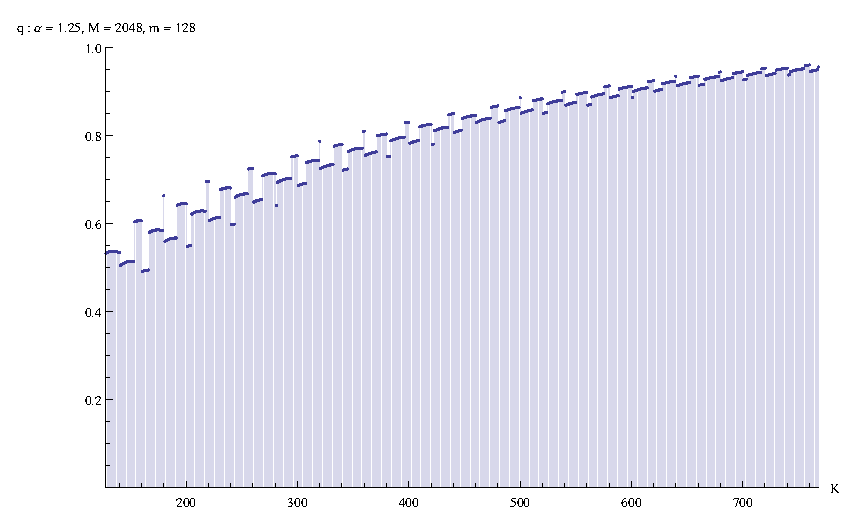
\includegraphics{figures/hyper}
\caption[Plot of probability that test set is ``stratified enough'']{Probability $q$ that test set is ``stratified enough''.
$K$ is the number of positive samples in original data set.}
\label{fig:hyper}
\end{center}
\end{figure}


% FIXME!!
\begin{table}
\begin{small}
\begin{center}
\begin{tabular}{lrrrrrl}
\textbf{GO id} & $K$ & \textbf{Ratio} & $q_{\alpha = 1.1}$ & $q_{\alpha = 1.25} $ & $q_{\alpha = 1.5}$ &  \textbf{Name} \\ \hline
GO:0003674  &  2048  &  1.00  & 1.00 & 1.00 & 1.00 &    molecular function \\ \hline
GO:0003824  &  764   &  0.37  & 0.60 & 0.95 & 1.00 &    catalytic activity \\ \hline
GO:0005488  &  1627  &  0.79  & 0.97 & 1.00 & 1.00 &    binding \\ \hline
GO:0005515  &  731   &  0.36  & 0.61 & 0.95 & 1.00 &   protein binding \\ \hline
GO:0016740  &  285   &  0.14  & 0.31 & 0.70 & 0.94 &   transferase activity \\ \hline
GO:0016787  &  290   &  0.14  & 0.31 & 0.70 & 0.93 &   hydrolase activity \\ \hline
GO:0036094  &  325   &  0.16  & 0.38 & 0.73 & 0.95 &    small molecule binding \\ \hline
GO:0043167  &  717   &  0.35  & 0.61 & 0.95 & 1.00 &    ion binding \\ \hline
GO:0097159  &  806   &  0.39  & 0.65 & 0.96 & 1.00 &    organic cyclic compound binding \\ \hline
GO:0097367  &  186   &  0.09  & 0.25 & 0.56 & 0.87 &   carbohydrate derivative binding \\ \hline
GO:1901363  &  797   &  0.39  & 0.60 & 0.97 & 1.00 &   heterocyclic compound binding \\ \hline
GO:0001882  &  156   &  0.08  & 0.27 & 0.61 & 0.81 &  nucleoside binding \\ \hline
GO:0003676  &  611   &  0.30  & 0.57 & 0.91 & 1.00 &    nucleic acid binding \\ \hline
GO:0005102  &  148   &  0.07  & 0.27 & 0.51 & 0.76 &    receptor binding \\ \hline
GO:0043168  &  256   &  0.12  & 0.32 & 0.72 & 0.93 &   anion binding \\ \hline
GO:0043169  &  520   &  0.25  & 0.47 & 0.88 & 0.99 &   cation binding \\ \hline
GO:1901265  &  279   &  0.14  & 0.40 & 0.71 & 0.94 &    nucleoside phosphate binding \\ \hline
GO:0000166  &  279   &  0.14  & 0.40 & 0.71 & 0.94 &    nucleotide binding \\ \hline
GO:0001883  &  153   &  0.07  & 0.27 & 0.51 & 0.81 &    purine nucleoside binding \\ \hline
GO:0003677  &  221   &  0.11  & 0.34 & 0.61 & 0.87 &    DNA binding \\ \hline
GO:0003723  &  199   &  0.10  & 0.24 & 0.64 & 0.86 &   RNA binding \\ \hline
GO:0032549  &  152   &  0.07  & 0.27 & 0.51 & 0.81 &    ribonucleoside binding \\ \hline
GO:0035639  &  148   &  0.07  & 0.27 & 0.51 & 0.76 &  purine ribonucleoside triphosphate binding \\ \hline
GO:0046872  &  507   &  0.25  & 0.47 & 0.86 & 0.99 &    metal ion binding \\ \hline
GO:0017076  &  154   &  0.08  & 0.27 & 0.60 & 0.81 &    purine nucleotide binding \\ \hline
GO:0032550  &  151   &  0.07  & 0.27 & 0.51 & 0.80 &   purine ribonucleoside binding \\ \hline
GO:0032553  &  157   &  0.08  & 0.27 & 0.61 & 0.82 & ribonucleotide binding \\ \hline
GO:0046914  &  220   &  0.11  & 0.34 & 0.70 & 0.87 &    transition metal ion binding \\ \hline
GO:0008270  &  185   &  0.09  & 0.25 & 0.56 & 0.87 &    zinc ion binding \\ \hline
GO:0030554  &  132   &  0.06  & 0.28 & 0.54 & 0.78 &   adenyl nucleotide binding \\ \hline
GO:0032555  &  153   &  0.07  & 0.27 & 0.51 & 0.81 &    purine ribonucleotide binding \\ \hline
GO:0032559  &  131   &  0.06  & 0.28 & 0.54 & 0.78 &   adenyl ribonucleotide binding \\ \hline
\end{tabular}
\end{center}
\end{small}
\caption{Counts of positive samples in the data set for each function.}
\label{table:terms}
\end{table}

Finally, let us remark that although cross-validation is normally used only to evaluate
the classifier performance and the final classifier is produced by training 
on the whole set, this is not done here.
The reasons are two: First the learning is already very computationally demanding
and this would make it even more and second, this work
is intended to be experimental only and the classifier will not be 
immediately applied, so it would not be useful anyway.

%*****************************************************************************
\chapter{Realization and implementation}
\label{ch:realization}
In this chapter, more technical details about the actual implementation 
of the ideas described in the previous chapter are discussed.

\section{Requirements} implementation of this work was done using combinations of Bash shell scripts
and novel software written in the Python programming language.
The scikit-learn \cite{sklearn} library was used as 
implementation of machine learning algorithms including SVM, cross validation and receiver operating characteristic evaluation.
The BayesPy (\url{http://www.bayespy.org/}) library is used for representation and inference of 
the correcting Bayesian networks.
The Matplotlib library is used to create figures presented in the results chapter \ref{ch:results}.
The dill library is necessary for data serialization done for speed and memory optimizations.
Python version $\ge$ 3.5 is required.
Finally a crucial component is the TreeLiker software,
used as RelF implementation,
which is a standalone third party product. (\url{http://ida.felk.cvut.cz/treeliker/TreeLiker.html})


\section{Environment preparation} The implementation of this work can be divided into two parts that can be ran independently once some data are present:
1) Scripts that download and prepare the data.
2) Python script that performs the learning and evaluation.
We will first describe the data preparation.

First of all, the project should be configured in the \texttt{config.sh} file,
which contains mainly names of data source files and numerical parameters
such as the required data set size and so on.
There is a sample configuration file present with the name \texttt{config-sample.sh},
which should be self-explanatory and can be copied to \texttt{config.sh}.

Then the data are downloaded from the sources mentioned in section \ref{sec:data}.
Notice, that the entire PDB archives (a gzipped xml file for each of the $\approx$ 110000 protein entries)
available for download using \texttt{rsync} tool add up to 42GiB to this date,
which may take a long time to download.
This can be done by running the \texttt{updatadata.sh} script.

Once the data are downloaded, the \texttt{blastdb.sh} script can be ran,
which filters the protein entries as described in subsection \ref{ssec:proteins}
and calculates pairwise BLAST distances. 
This is done using the offline BLAST+ software package
available at \url{ftp://ftp.ncbi.nlm.nih.gov/blast/executables/blast+/2.2.31/}
and running the \texttt{makeblastdb} and \texttt{blastp} commands. 
(See the script for details.)
The filtering results in $n > 40000$ candidate proteins.
Computing pairwise BLAST distance requires $O(n^2)$ local alignment computations.
That is a lengthy computation which took about four hours on a 3.1 GHz processor.
The results are stored and a non-redundant data set 
is generated from the candidate set using the method described in \ref{ssec:redundancy}.
The non-redundant data set can be also generated independently using the 
\texttt{dp/maximumIndependentSet.py} script.

Before the project environment is completely ready,
the script \texttt{updatadata.sh} has to be run once more before first run to prepare
serialized associations for the main program which enables it to run faster.
Then, the \texttt{run.sh} script can be ran.
(Alternatively \texttt{main.py} can be ran instead, but parameters
are not taken from \texttt{config.sh} and have to be entered in command line,
use \texttt{main.py $--$help} for details.)
There is one serious performance issue:
Depending on the protein entry size,
it can take several seconds to decompress and parse a single one.
For this reason, once parsed, the relevant data
(name, primary structure, secondary structure information and distances
between amino acid residues) is serialized and stored.
When the protein data are requested again, even in subsequent 
runs of the program, it is available quickly.

\section{Main processing}
When ran, the program first parses the ontology in the obo format and the protein annotation file
automatically downloaded previously from Gene Ontology servers.
It clips the data set to the required maximal size and decides which
protein functions have enough positive examples in order to be studied.
For each of these functions a copy of the data set 
with the function's respective labels is
converted to the 
relational format described in \ref{ssec:relrepr} in the ``pseudo-prolog''
syntax understood by TreeLiker.
A TreeLiker batch file describing how the propositionalization
should exactly be performed including cross validation considerations
is also generated.
Then, the TreeLiker software is called as a sub-process.
That is the most computationally demanding part of the data flow.
In the described settings, it ran for approximately 23 hours for each function.
(That is almost 3 hours per cross-validation fold.)
Multiplied by 31 studied protein functions, it adds up to a month of computation time.
For this reason, the computations were run in parallel 
using the MetaCentrum/CERIT-SC computational facilities.
The intermediate results produced by TreeLiker in arff format are bzip2 compressed
and since they are text files the compression rate is very high. 
Without compression, the size of the entire working directory
would exceed the CERIT-SC (zuphux front-end machine) 104GiB disc quota.
When the propositionalization is finished,
the SVM classifiers are trained for each fold
and subsequently the correcting Bayesian networks are produced.
The source code in \texttt{dp/learn.py}
allows easily to add and examine different types of classifiers 
or classifiers with different parameters supported 
by scikit-learn in the \texttt{classifiers} variable
in \texttt{learningTest} function.
Then, evaluation on kept-aside validation data is performed
and plotted ROC curve figures are saved
in the \texttt{results} folder.


%*****************************************************************************
\chapter{Experimental results}
\label{ch:results}

In this chapter, 
the performance of the classifiers in 
general and comparison of performance on different functions
is explored. 
The features (structural patterns) generated during propositionalization are examined.
Classification results without consistency correction are compared to
corrected results.
The classification quality metric used here is the area under curve (AUC)
of receiver operating characteristic (ROC).
In summary, the results show that
the prediction precision varies depending on the function being predicted,
but for all functions, it preforms better than random. 
The consistency correction however, did not improve the classification precision.

First, let us have a look at the bad news: 
Unlike in the work \cite{bnet},
the consistency correction did not make the classification 
any better,
in fact it made it worse for all studied functions.
See Figure \ref{fig:roc_corrected}, which shows a really poor ROC curves
for the corrected classification.
\begin{figure}[h]\begin{center}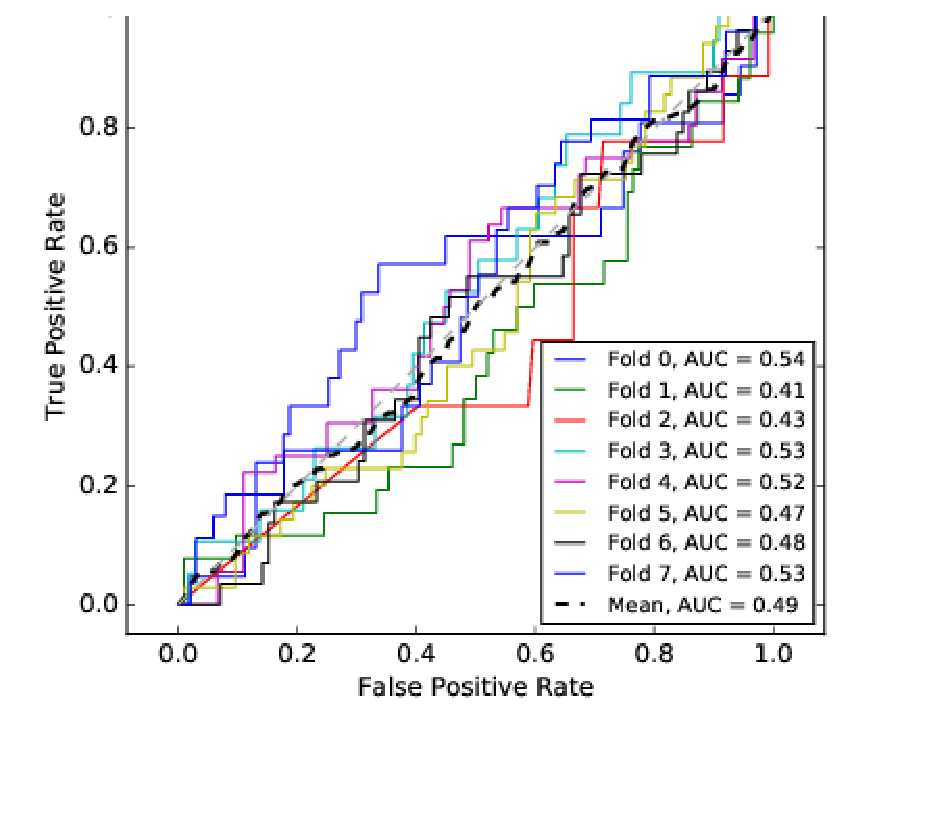
\includegraphics[width=0.5\linewidth]{figures/binding-corrected}\captionof{figure}{Results for function ``binding'' with consistency correction}\label{fig:roc_corrected}\end{center}\end{figure}
With best AUC = 0.54 it is only slightly better than classifying at random
and considering that the mean AUC is actually 0.49,
the differences in AUC values on folds are possibly just random noise.
The ROC curves for other functions after correction look similar to figure \ref{fig:roc_corrected}, although the variance between folds is usually higher.
The possible cause for this is the following:
The prior probability $P(y_i)$ for a function is equal to it's ratio in the data set (see table \ref{table:terms}).
In case $P(y_i)$ is low (lower values are for more specific functions) and $\hat{y}_i$ is positive, but not very high
(i.e. it is classified as positive, but not with high certainty)
it will happen, that the final classification output will be negative,
although $\hat{y}_i$ is positive.
(But with lower certainty expressed by $P(y_i\, | \, \hat{y}_i)$ than if $\hat{y}_i$ were negative, of course.)
In other words, the class separation precision in the SVM classifier 
is unable to outweight the prior probability which says that ``most proteins do not belong to this specific class''.
This information then propagates even to less specific functions in the ontology during Bayesian inference.
The resulting output is then often ``no'' for all classes except most general ``molecular function'',
which is indeed consistent, but useless.
This could be potentially fixed by having the classifiers in individual functions much more precise
or using a different theoretical framework, which would enable us to bypass the low prior probabilities.

The possible important differences to the work \cite{bnet},
where the authors claim that the consistency correction actually made the classification better,
which could be factors to the classification quality include:
\begin{itemize}
 \item Very different input data. They used microarray gene expression data to train classifiers.
 \item They studied a larger subset of Gene Ontology.
 \item The used Bayesian inference algorithm is not explicitly stated in the article. It only says: ``...we can use any standard exact inference or simulation algorithm to find the most likely configuration...''
 \item Use of bagged SVM with bootstrapping instead of single SVM with cross validation is probably not too significant, but still could alter the results.
\end{itemize}


The good news is that without the correction, the classifiers gave a good results
for many specific functions. 
For more general functions, the classification is less precise.
Consider for example the results on figures \ref{fig:roc_zinc_ion_binding} (zinc ion binding),
\ref{fig:roc_ion_binding} (ion binding) and \ref{fig:roc_binding} (binding).
The more specific, the more precise.
That is understandable:
RelF can find a structural pattern in the protein that is captures a certain chemical configuration
that would be responsible for binding a zinc ion.
But a general binding site can be of much varying configurations and would have to be described 
by a disjunction of more features each of which would be relatively less frequent.
For example, the function ``ion binding'' contains both anion and cation binding,
which we can expect to have chemically different binding sites,
but the classifier for ``ion binding'' has to be able to cover both cases.
This results in the precision being generally lesser for less specific functions.
An example of exception to this rule is the ``catalytic activity'' function (Figure \ref{fig:roc_catalytic_activity})
which is actually one of the best classifying,
but both ``hydrolase activity'' (Figure \ref{fig:roc_hydrolase_activity}) and ``transferase activity''
(Figure \ref{fig:roc_transferase_activity}) 
are more specific and yet classified with worse precision.
The possible cause for that is that these specific functions simply have too small number of positive examples in the data set,
while ``catalytic activity'' contains significantly more positive examples than their union.

For the DNA-binding function, we can compare the results here to the results in \cite{szabova},
where similar method was used.
For SVM with RBF kernel, the result on 10-fold stratified cross validation was 0.83,
but for the best-performing classifier (logistic regression) it was 0.88.
Here, the best result in 8-fold cross validation for RBF SVM is 0.77,
which is significantly worse. 
This is possibly due to the more careful construction
of the data set in \cite{szabova}: 
The data set was constructed deliberately with the single studied function in mind 
and included only proteins in certain conformation while also
focusing on so-called zinc-finger proteins which have a specific DNA-binding mechanism.

Notice, how some of the figures (for example Figure \ref{fig:roc_purine_nucleoside_binding})
show exceptionally good ROC curve for one fold.
That unfortunately does not mean the classifier trained on this fold
is almost perfect, but that the train set in that fold does not contain 
enough positive examples,
because the cross-validation could not be stratified as described in the methodology section \ref{sec:method}.
For this reason, it would be reasonable here to take the mean or median AUC of 
the folds as a metric of the classifier's quality.

Let us also remind here some results, already mentioned earlier:
The ensemble classifiers AdaBoost (with decision trees) and Random Forest
were also examined and gave similar results as SVM.
SVMs with different values of $C$ or different kernel (linear, polynomial) did not seem to perform well.
Semi-supervised learning algorithms Label Propagation and Label Spreading \cite{semi}
with only positive samples labelled gave very poor results.
Deeper exploration of these topics would be interesting,
but it was beyond the scope of this work.

\section{Classifier performance plots}
In the following figures,
we can see in detail how the proposed method actually worked for each of the studied functions.

\begin{multicols}{2}
\begin{Figure}\begin{center}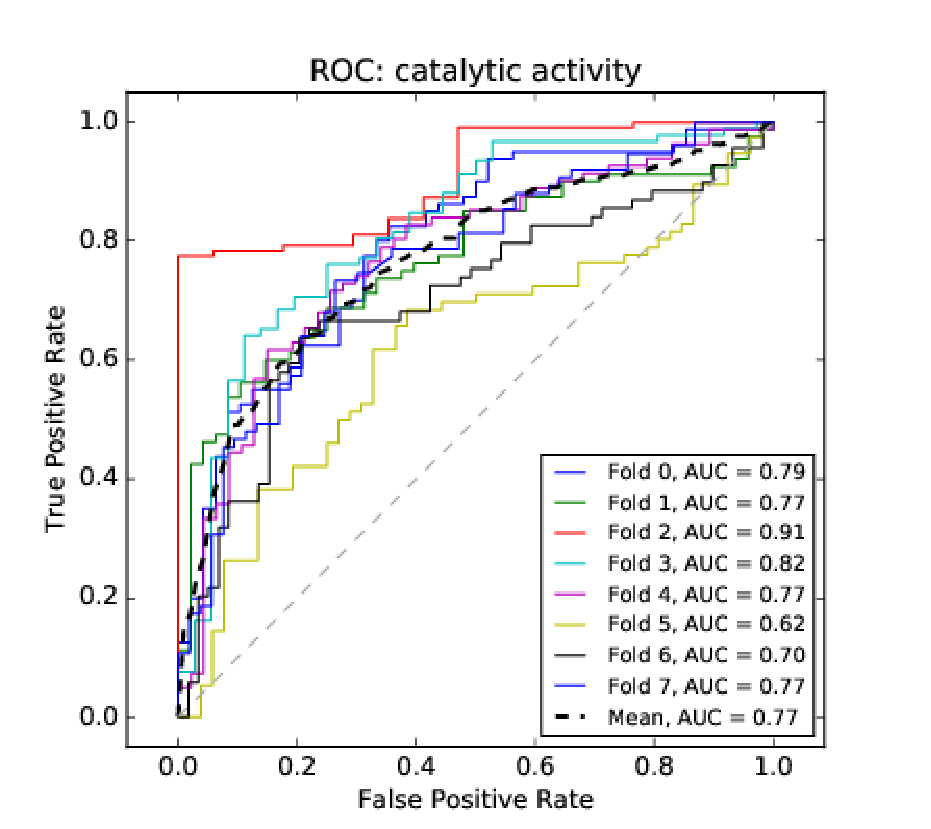
\includegraphics[width=\linewidth]{figures/roc_catalytic_activity}\captionof{figure}{Results for catalytic activity}\label{fig:roc_catalytic_activity}\end{center}\end{Figure}
\begin{Figure}\begin{center}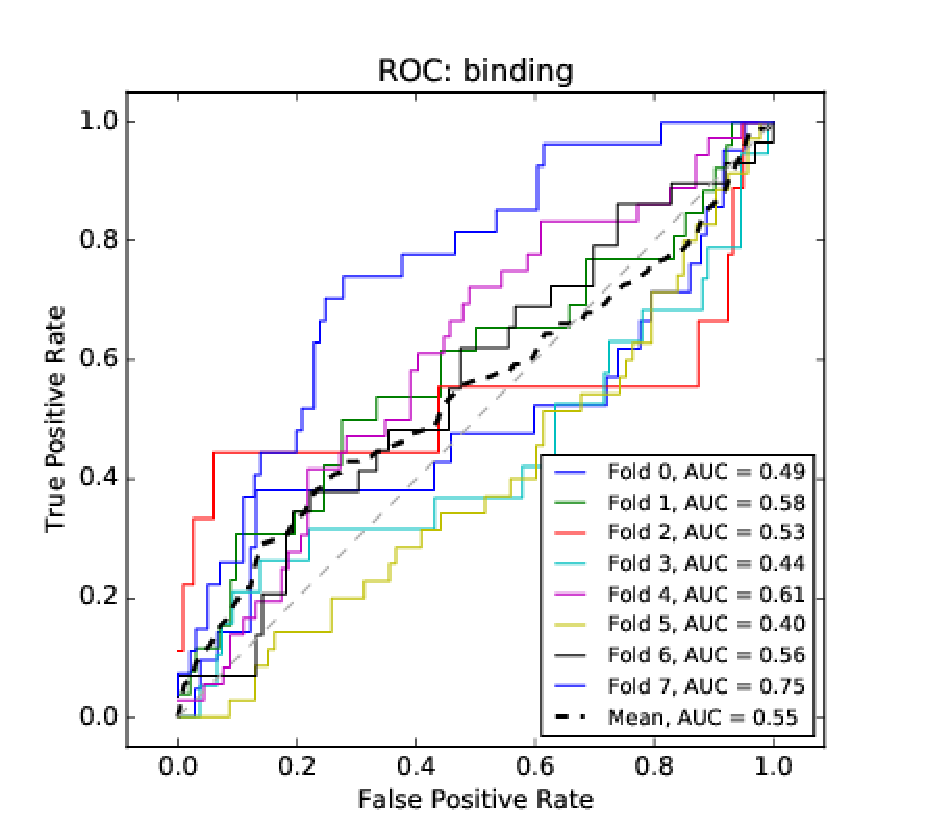
\includegraphics[width=\linewidth]{figures/roc_binding}\captionof{figure}{Results for binding}\label{fig:roc_binding}\end{center}\end{Figure}
\begin{Figure}\begin{center}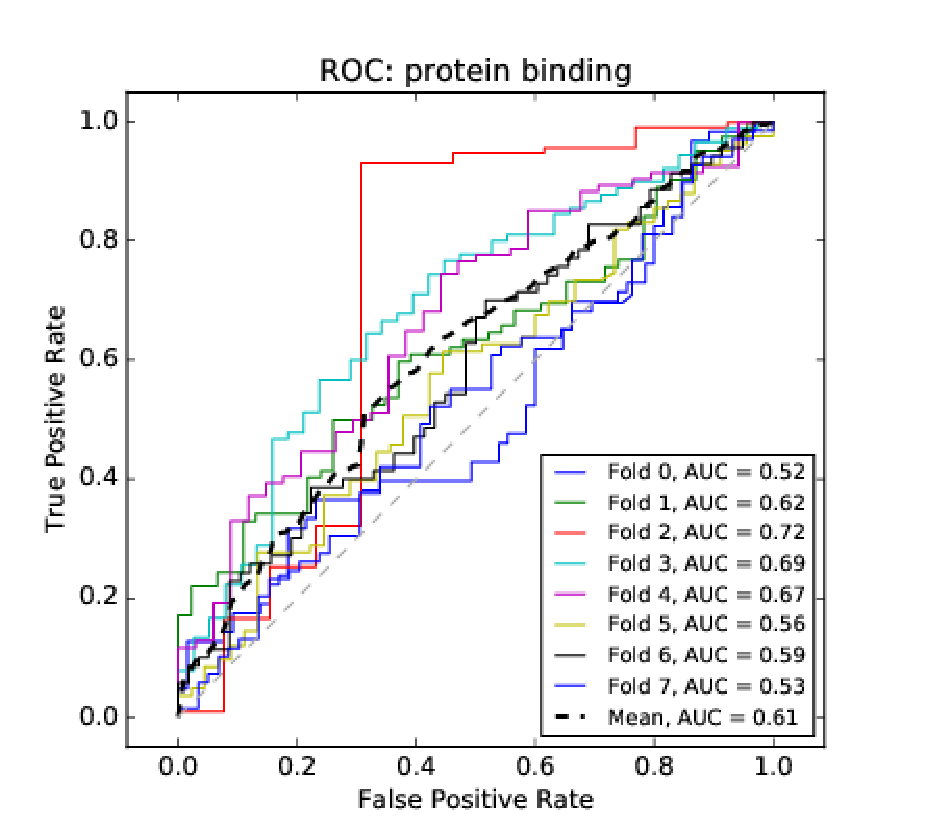
\includegraphics[width=\linewidth]{figures/roc_protein_binding}\captionof{figure}{Results for protein binding}\label{fig:roc_protein_binding}\end{center}\end{Figure}
\begin{Figure}\begin{center}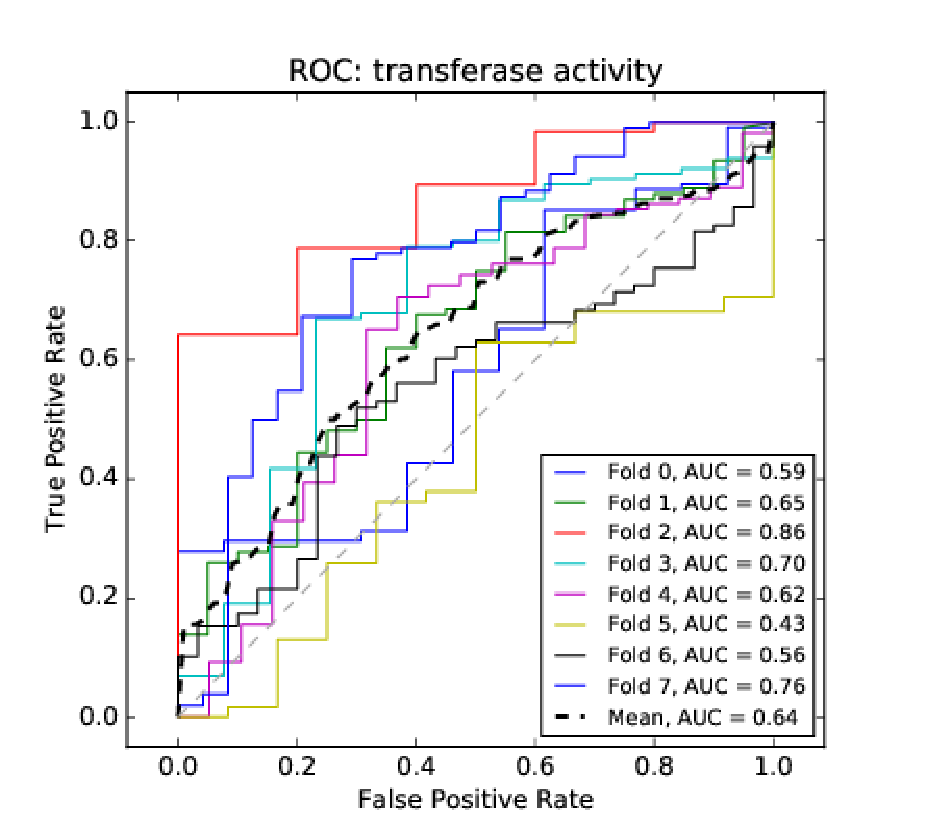
\includegraphics[width=\linewidth]{figures/roc_transferase_activity}\captionof{figure}{Results for transferase activity}\label{fig:roc_transferase_activity}\end{center}\end{Figure}
\begin{Figure}\begin{center}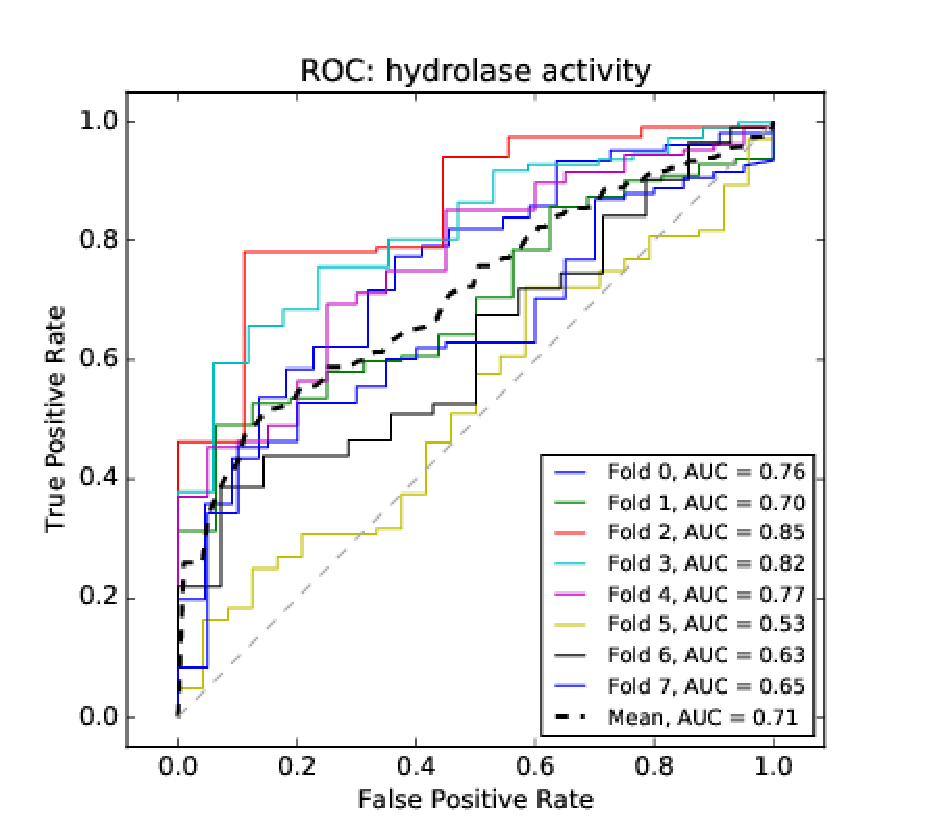
\includegraphics[width=\linewidth]{figures/roc_hydrolase_activity}\captionof{figure}{Results for hydrolase activity}\label{fig:roc_hydrolase_activity}\end{center}\end{Figure}
\begin{Figure}\begin{center}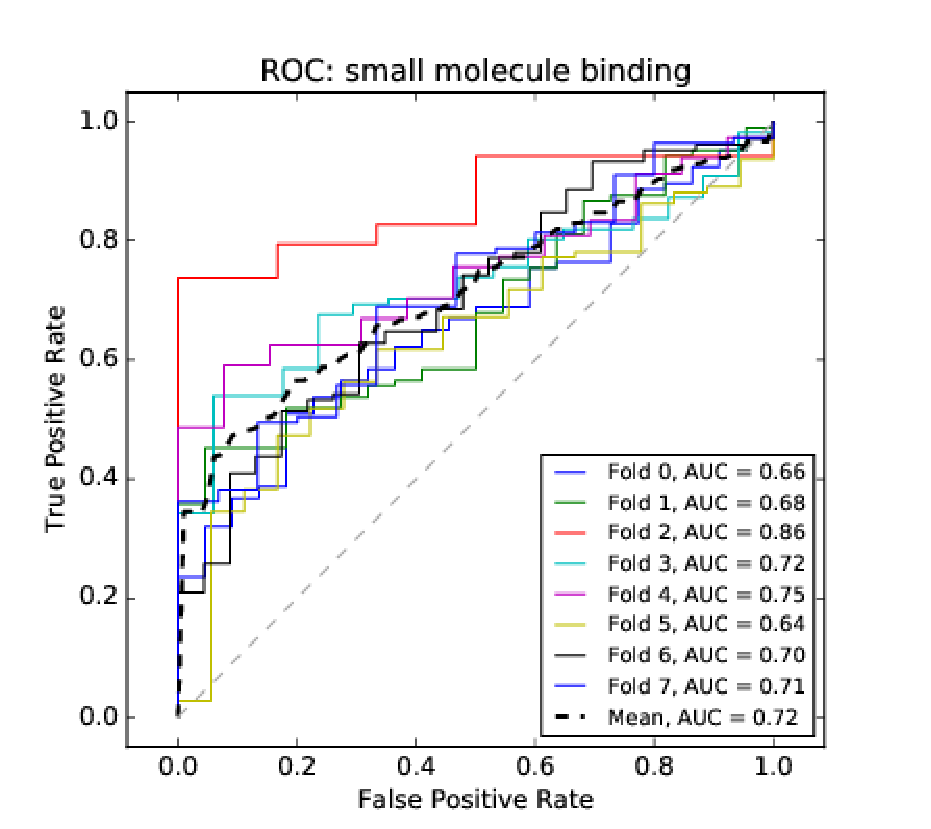
\includegraphics[width=\linewidth]{figures/roc_small_molecule_binding}\captionof{figure}{Results for small molecule binding}\label{fig:roc_small_molecule_binding}\end{center}\end{Figure}
\begin{Figure}\begin{center}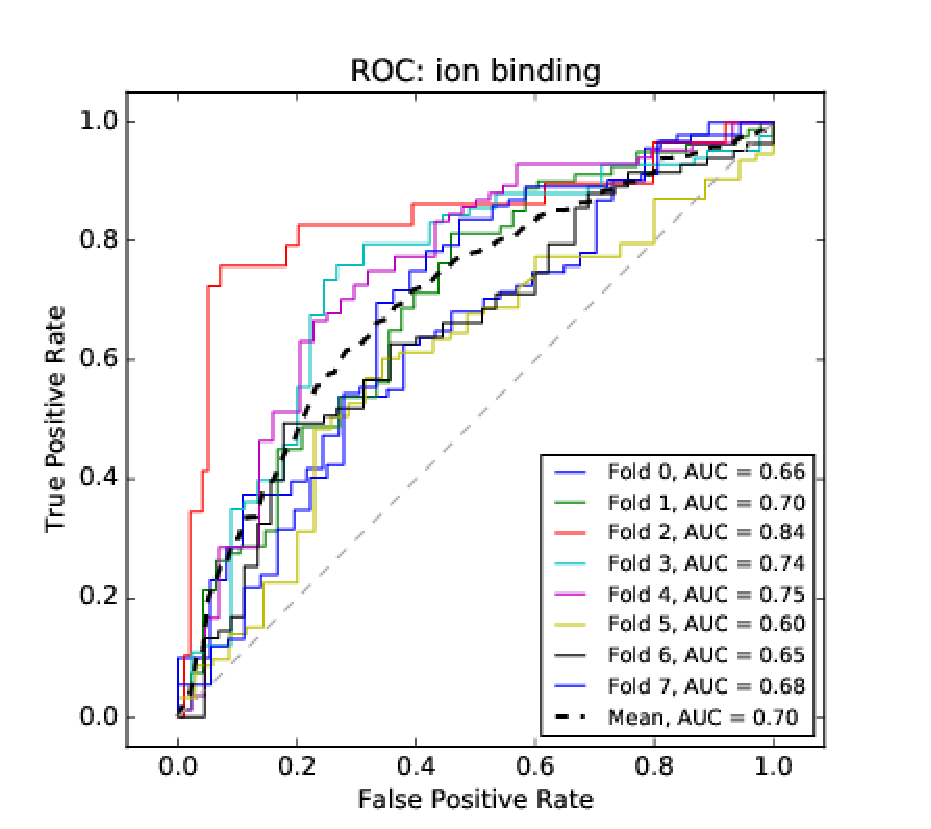
\includegraphics[width=\linewidth]{figures/roc_ion_binding}\captionof{figure}{Results for ion binding}\label{fig:roc_ion_binding}\end{center}\end{Figure}
\begin{Figure}\begin{center}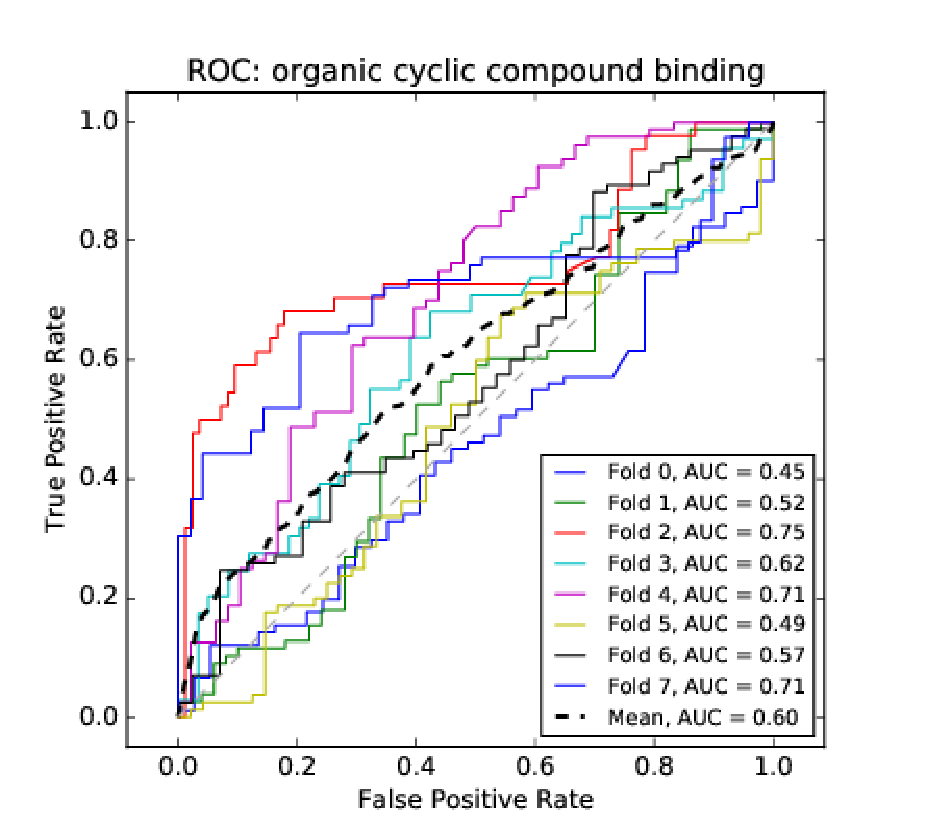
\includegraphics[width=\linewidth]{figures/roc_organic_cyclic_compound_binding}\captionof{figure}{Results for organic cyclic compound binding}\label{fig:roc_organic_cyclic_compound_binding}\end{center}\end{Figure}
\begin{Figure}\begin{center}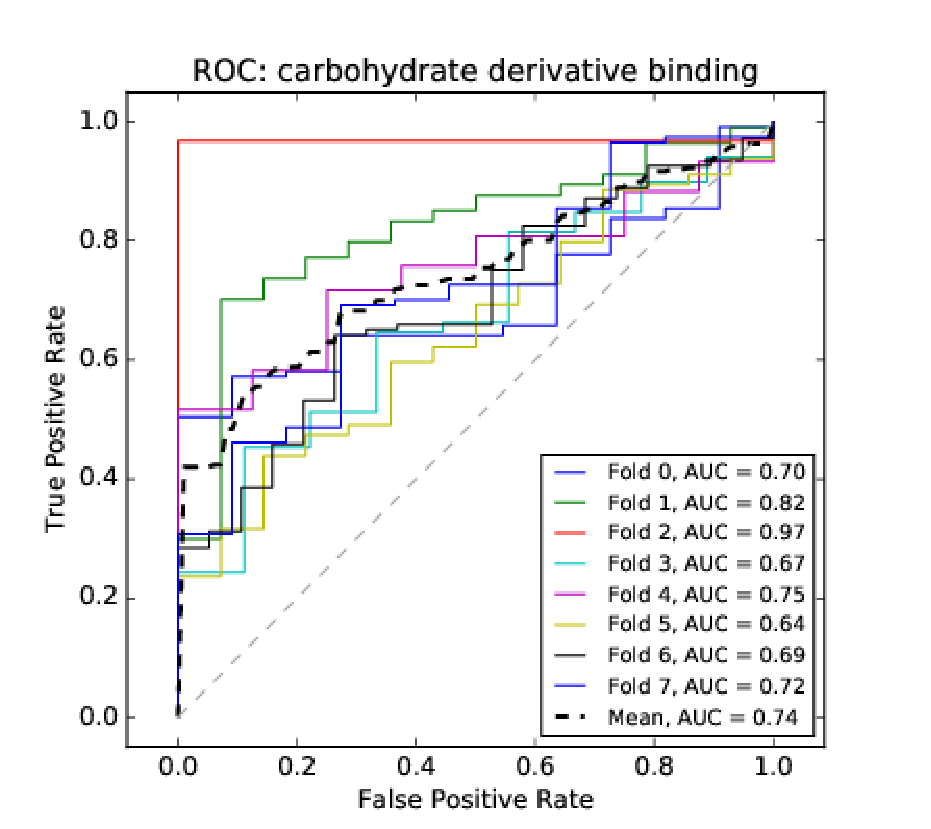
\includegraphics[width=\linewidth]{figures/roc_carbohydrate_derivative_binding}\captionof{figure}{Results for carbohydrate derivative binding}\label{fig:roc_carbohydrate_derivative_binding}\end{center}\end{Figure}
\begin{Figure}\begin{center}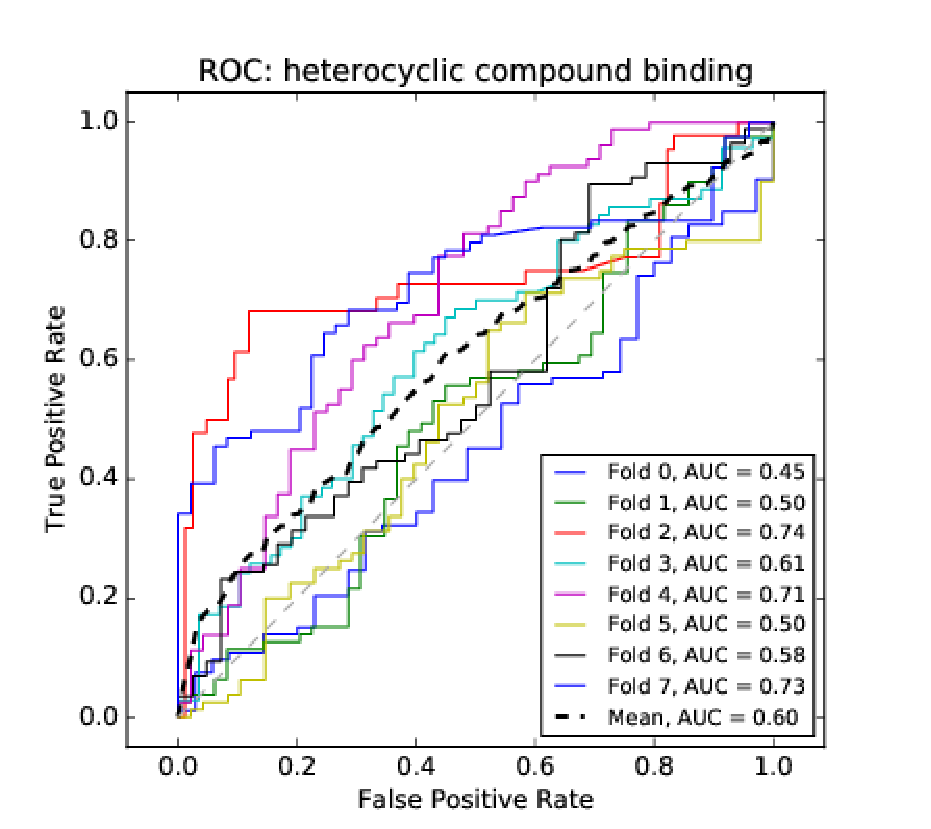
\includegraphics[width=\linewidth]{figures/roc_heterocyclic_compound_binding}\captionof{figure}{Results for heterocyclic compound binding}\label{fig:roc_heterocyclic_compound_binding}\end{center}\end{Figure}
\begin{Figure}\begin{center}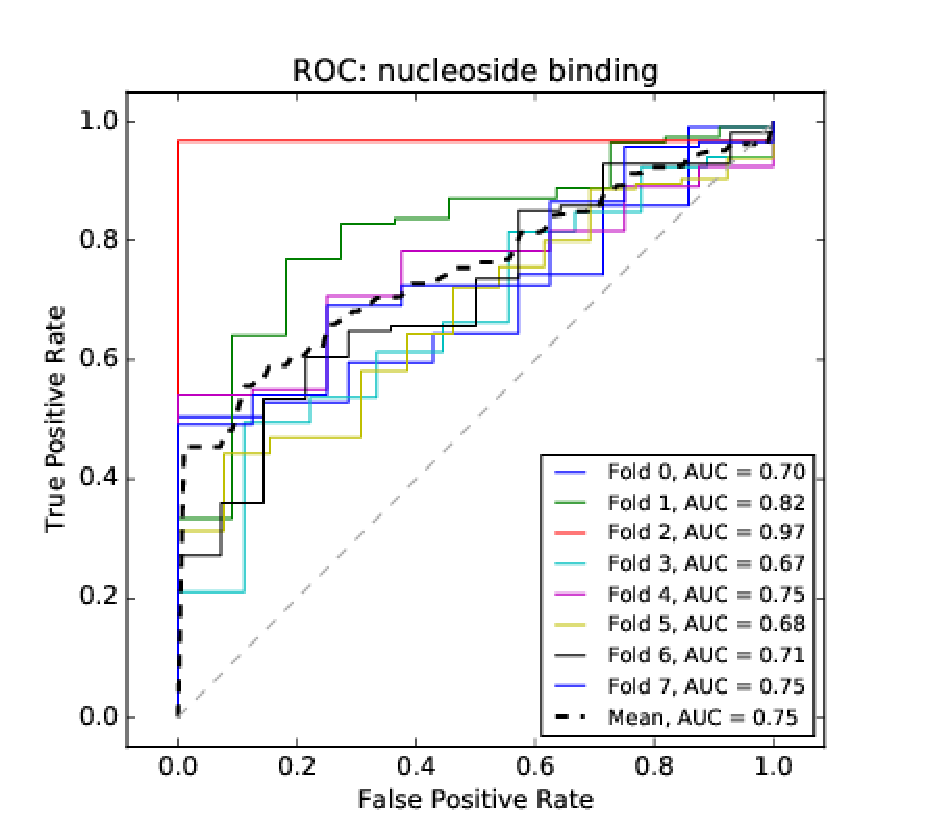
\includegraphics[width=\linewidth]{figures/roc_nucleoside_binding}\captionof{figure}{Results for nucleoside binding}\label{fig:roc_nucleoside_binding}\end{center}\end{Figure}
\begin{Figure}\begin{center}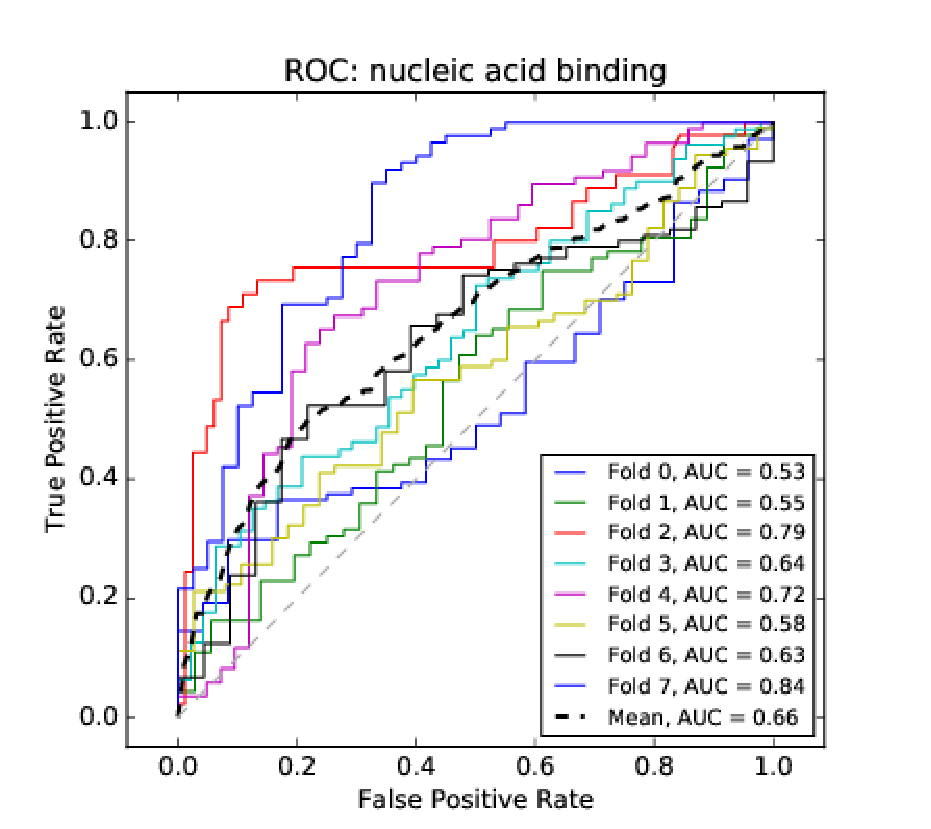
\includegraphics[width=\linewidth]{figures/roc_nucleic_acid_binding}\captionof{figure}{Results for nucleic acid binding}\label{fig:roc_nucleic_acid_binding}\end{center}\end{Figure}
\begin{Figure}\begin{center}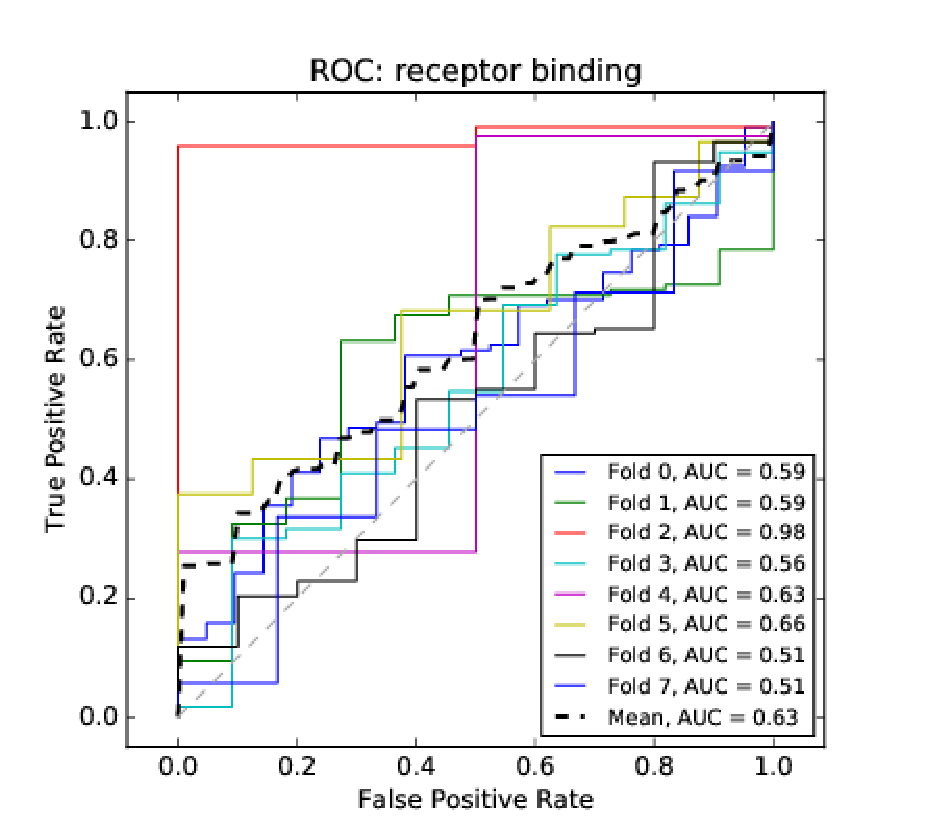
\includegraphics[width=\linewidth]{figures/roc_receptor_binding}\captionof{figure}{Results for receptor binding}\label{fig:roc_receptor_binding}\end{center}\end{Figure}
\begin{Figure}\begin{center}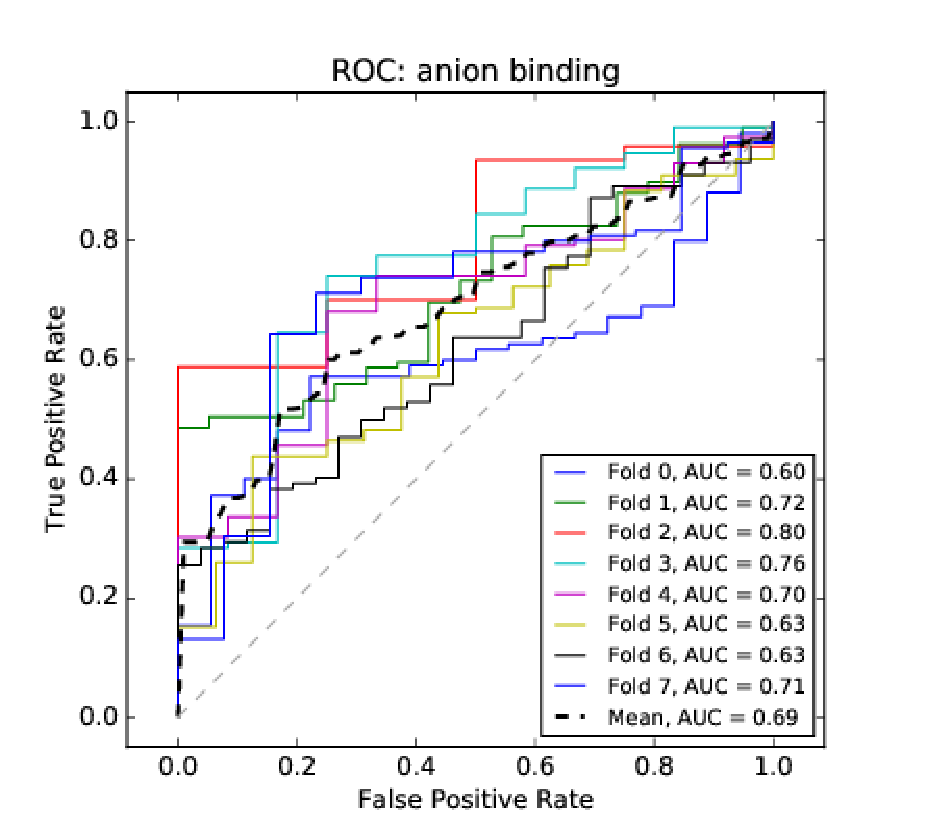
\includegraphics[width=\linewidth]{figures/roc_anion_binding}\captionof{figure}{Results for anion binding}\label{fig:roc_anion_binding}\end{center}\end{Figure}
\begin{Figure}\begin{center}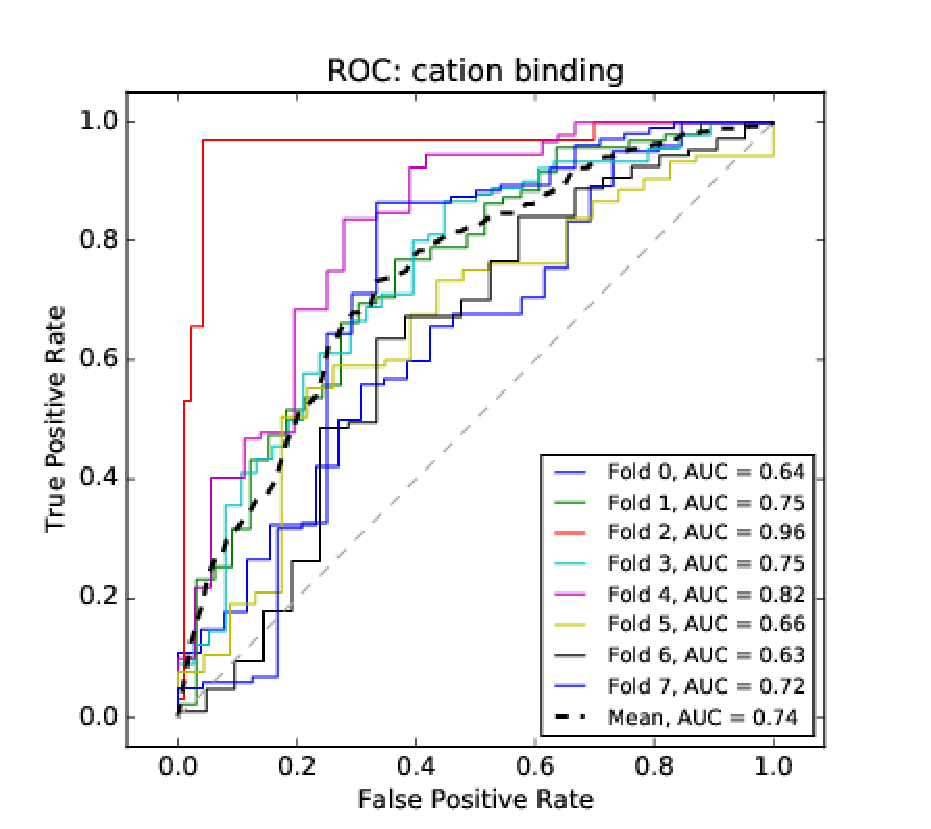
\includegraphics[width=\linewidth]{figures/roc_cation_binding}\captionof{figure}{Results for cation binding}\label{fig:roc_cation_binding}\end{center}\end{Figure}
\begin{Figure}\begin{center}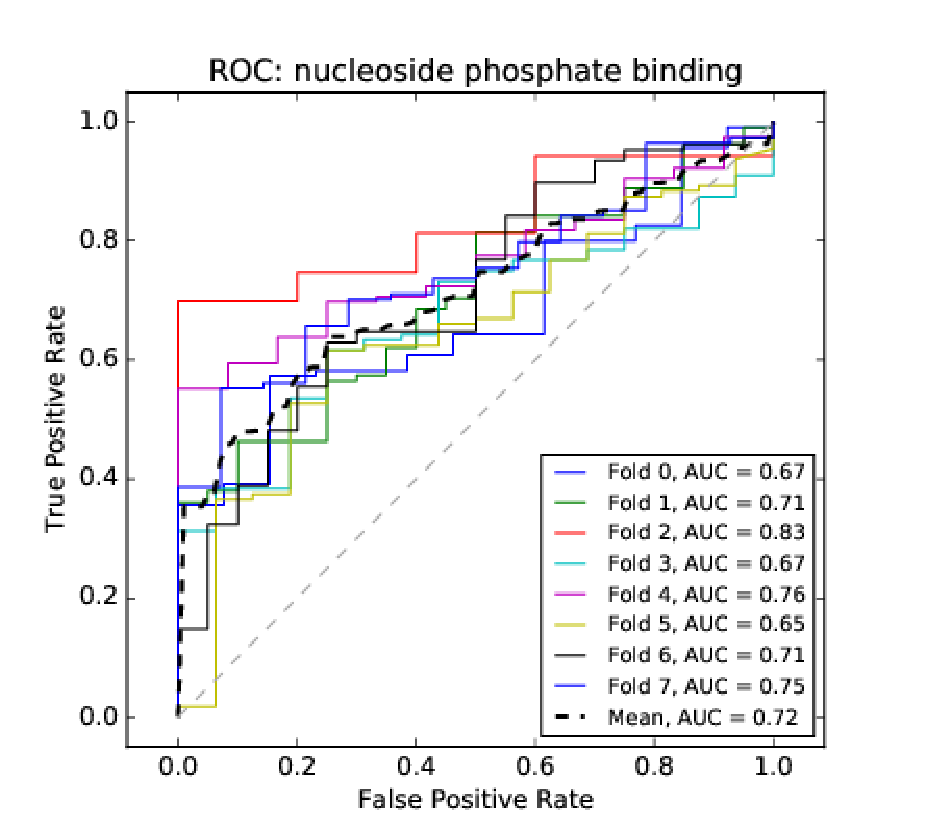
\includegraphics[width=\linewidth]{figures/roc_nucleoside_phosphate_binding}\captionof{figure}{Results for nucleoside phosphate binding}\label{fig:roc_nucleoside_phosphate_binding}\end{center}\end{Figure}
\begin{Figure}\begin{center}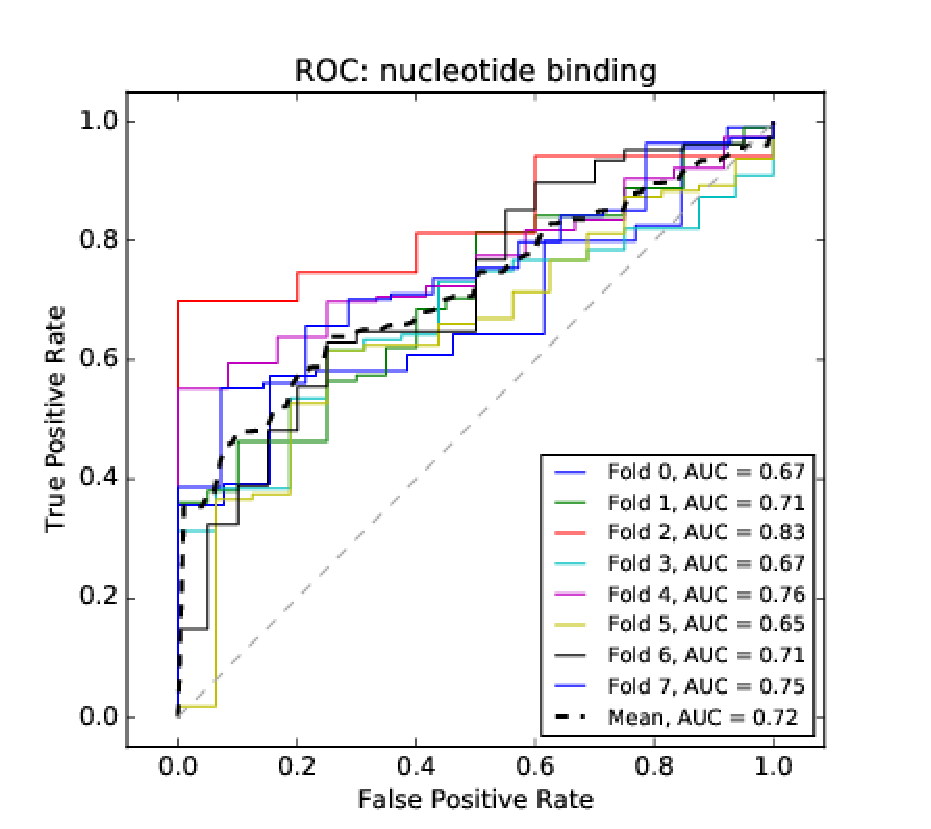
\includegraphics[width=\linewidth]{figures/roc_nucleotide_binding}\captionof{figure}{Results for nucleotide binding}\label{fig:roc_nucleotide_binding}\end{center}\end{Figure}
\begin{Figure}\begin{center}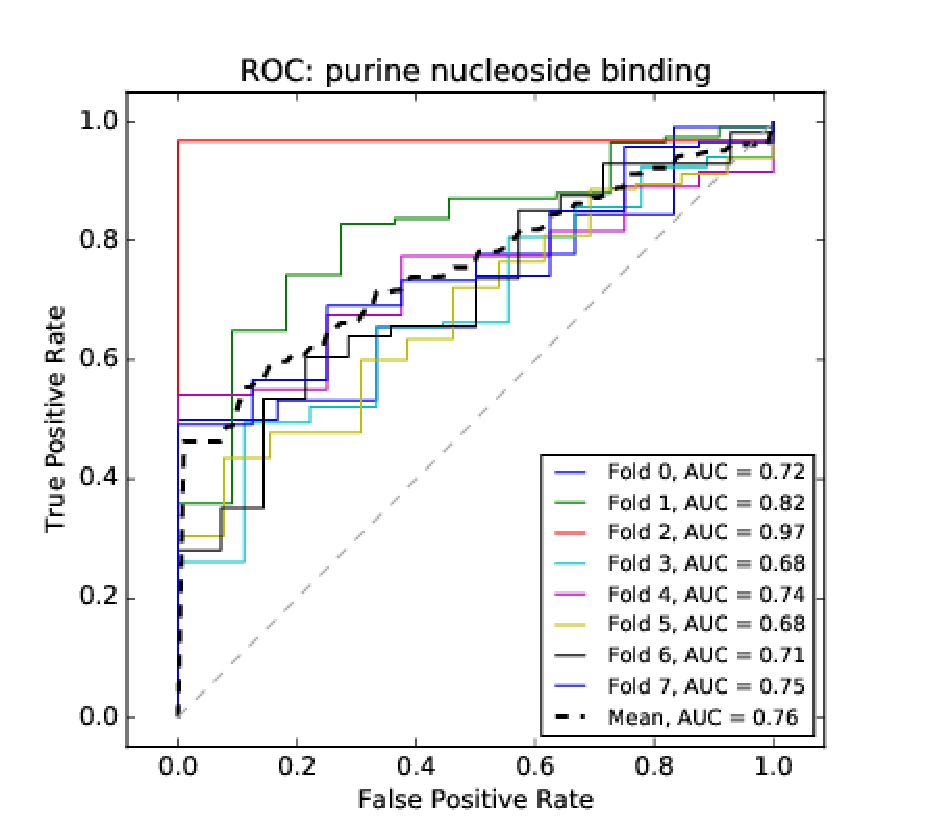
\includegraphics[width=\linewidth]{figures/roc_purine_nucleoside_binding}\captionof{figure}{Results for purine nucleoside binding}\label{fig:roc_purine_nucleoside_binding}\end{center}\end{Figure}
\begin{Figure}\begin{center}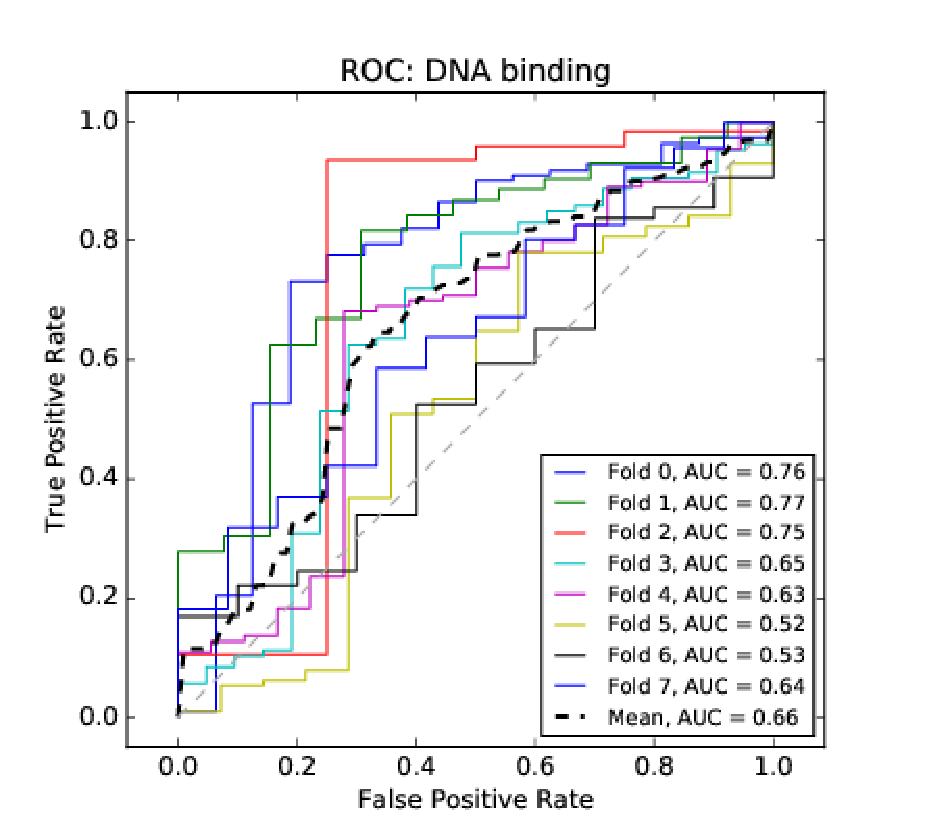
\includegraphics[width=\linewidth]{figures/roc_DNA_binding}\captionof{figure}{Results for DNA binding}\label{fig:roc_DNA_binding}\end{center}\end{Figure}
\begin{Figure}\begin{center}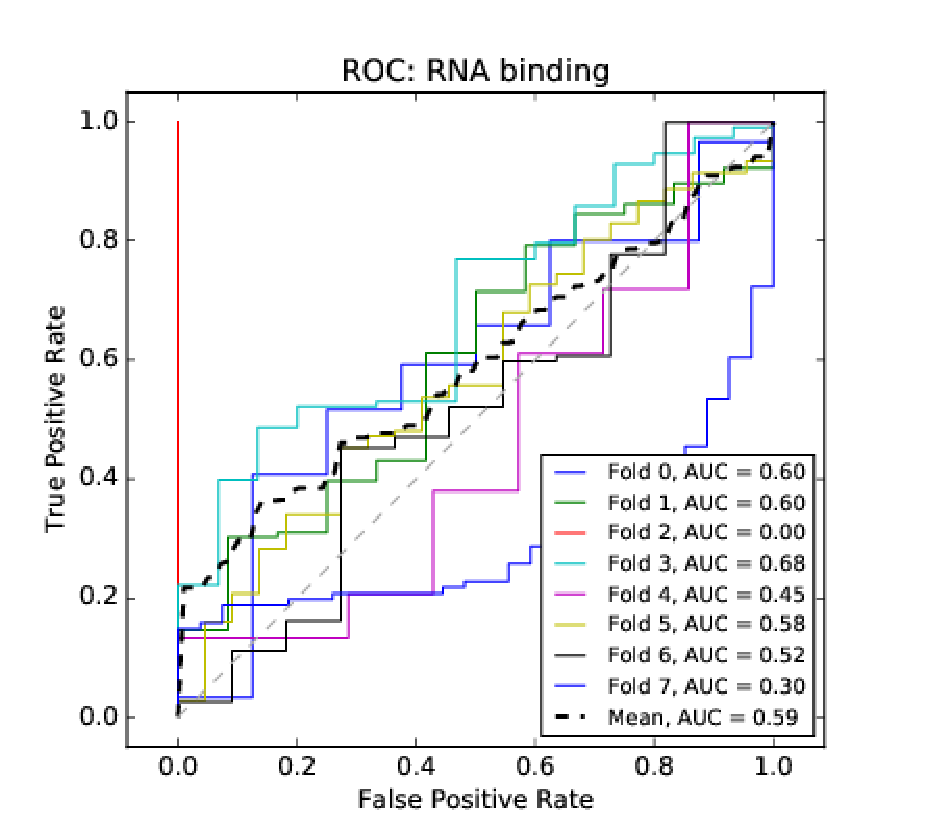
\includegraphics[width=\linewidth]{figures/roc_RNA_binding}\captionof{figure}{Results for RNA binding}\label{fig:roc_RNA_binding}\end{center}\end{Figure}
\begin{Figure}\begin{center}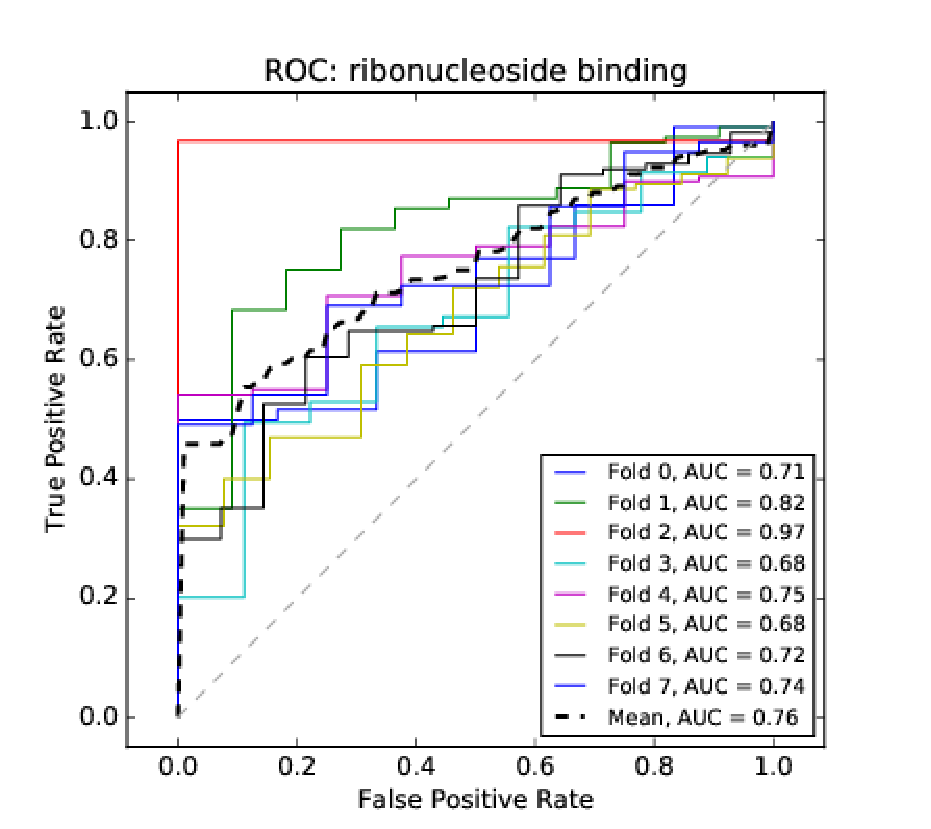
\includegraphics[width=\linewidth]{figures/roc_ribonucleoside_binding}\captionof{figure}{Results for ribonucleoside binding}\label{fig:roc_ribonucleoside_binding}\end{center}\end{Figure}
\begin{Figure}\begin{center}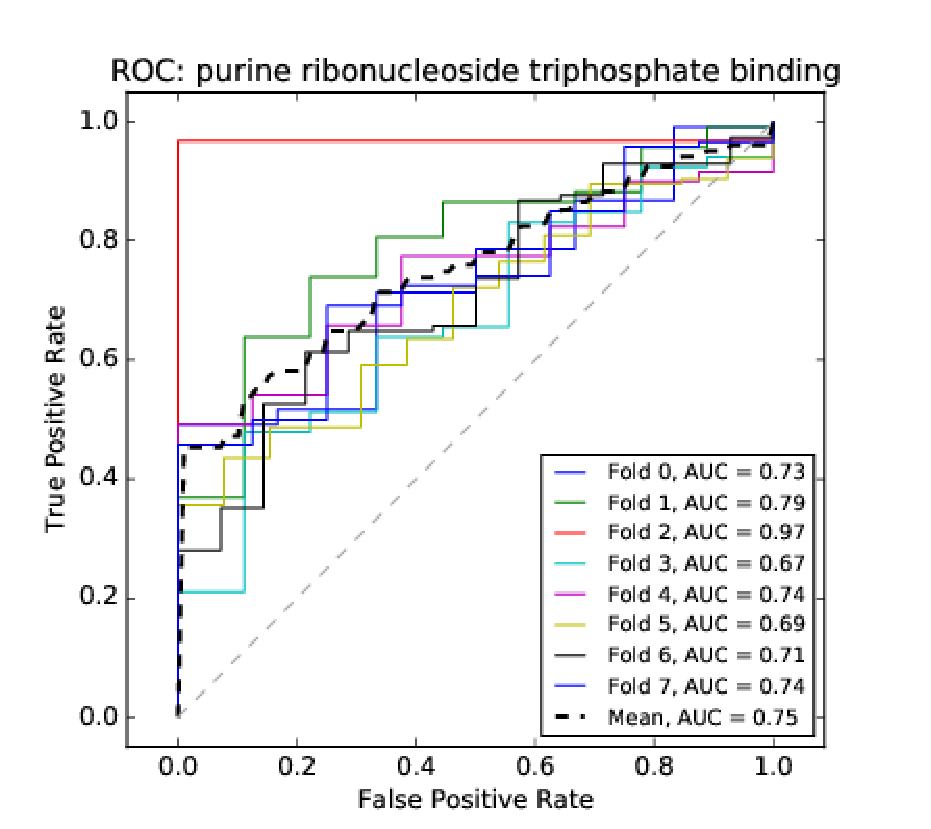
\includegraphics[width=\linewidth]{figures/roc_purine_ribonucleoside_triphosphate_binding}\captionof{figure}{Results for purine ribonucleoside triphosphate binding}\label{fig:roc_purine_ribonucleoside_triphosphate_binding}\end{center}\end{Figure}
\begin{Figure}\begin{center}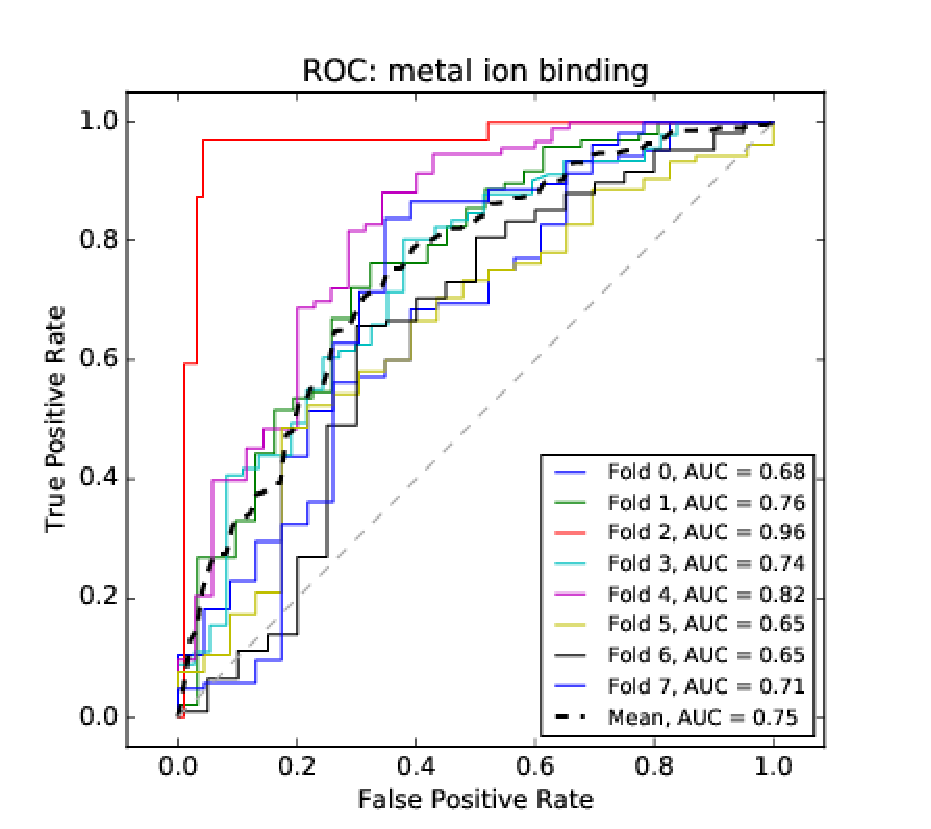
\includegraphics[width=\linewidth]{figures/roc_metal_ion_binding}\captionof{figure}{Results for metal ion binding}\label{fig:roc_metal_ion_binding}\end{center}\end{Figure}
\begin{Figure}\begin{center}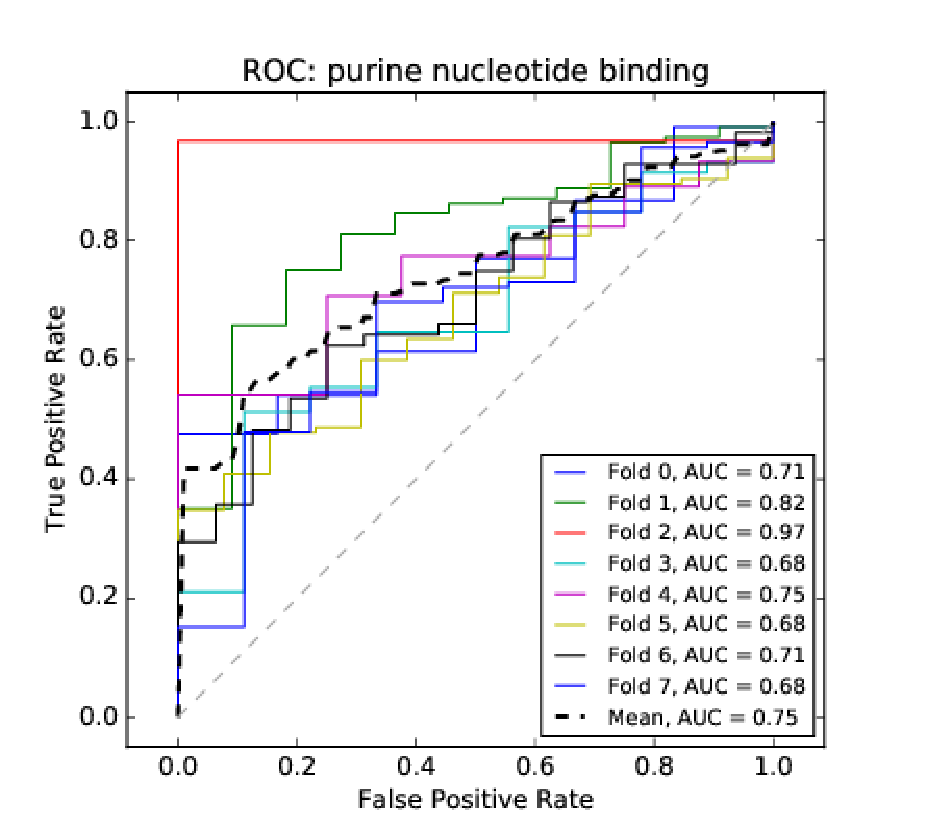
\includegraphics[width=\linewidth]{figures/roc_purine_nucleotide_binding}\captionof{figure}{Results for purine nucleotide binding}\label{fig:roc_purine_nucleotide_binding}\end{center}\end{Figure}
\begin{Figure}\begin{center}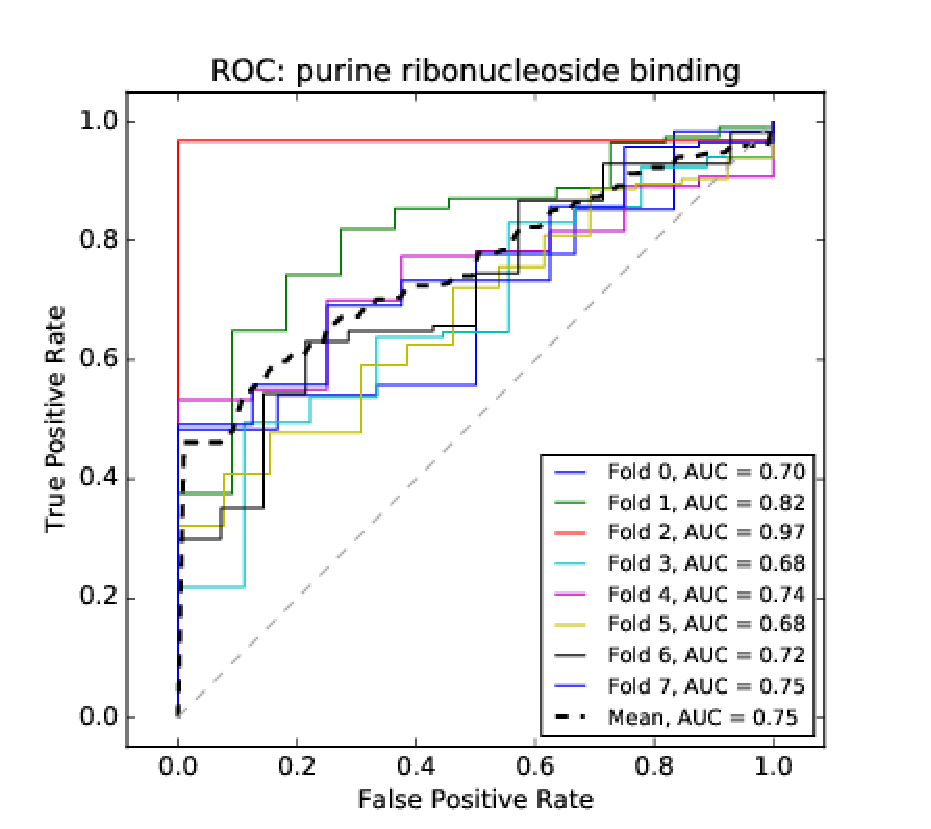
\includegraphics[width=\linewidth]{figures/roc_purine_ribonucleoside_binding}\captionof{figure}{Results for purine ribonucleoside binding}\label{fig:roc_purine_ribonucleoside_binding}\end{center}\end{Figure}
\begin{Figure}\begin{center}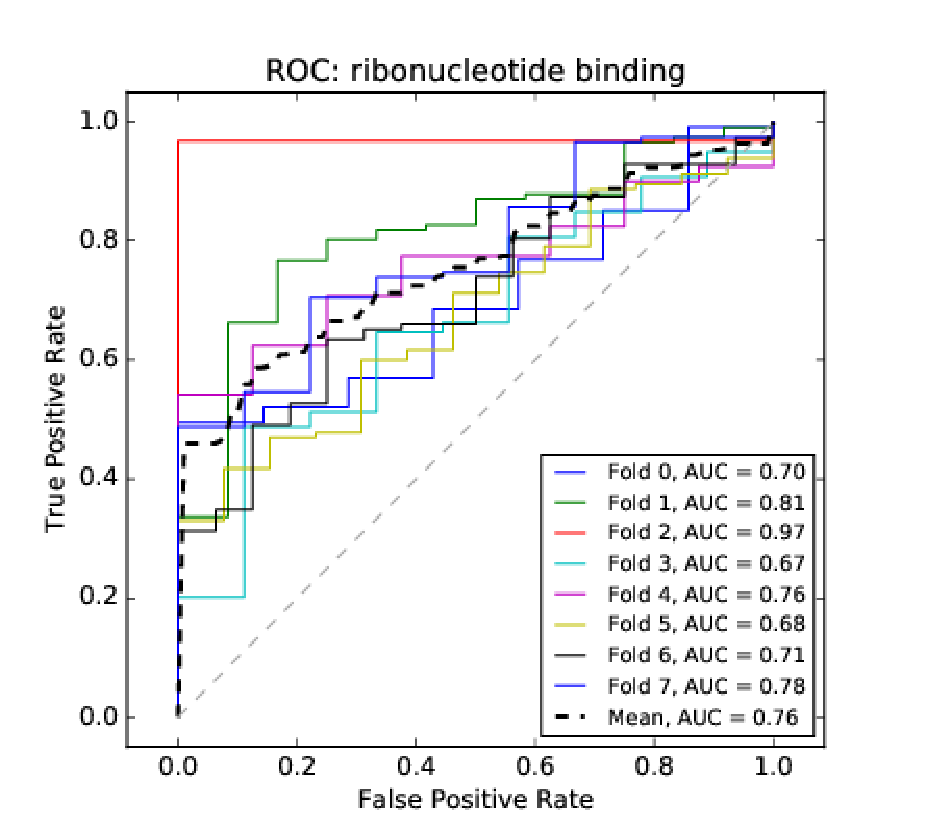
\includegraphics[width=\linewidth]{figures/roc_ribonucleotide_binding}\captionof{figure}{Results for ribonucleotide binding}\label{fig:roc_ribonucleotide_binding}\end{center}\end{Figure}
\begin{Figure}\begin{center}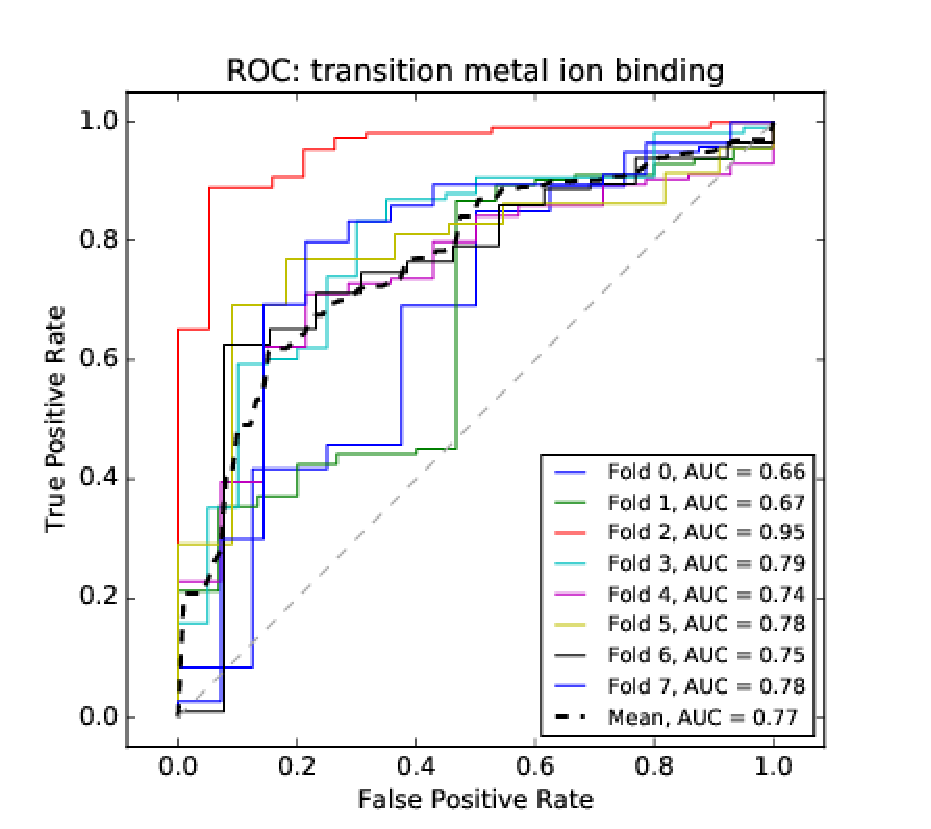
\includegraphics[width=\linewidth]{figures/roc_transition_metal_ion_binding}\captionof{figure}{Results for transition metal ion binding}\label{fig:roc_transition_metal_ion_binding}\end{center}\end{Figure}
\begin{Figure}\begin{center}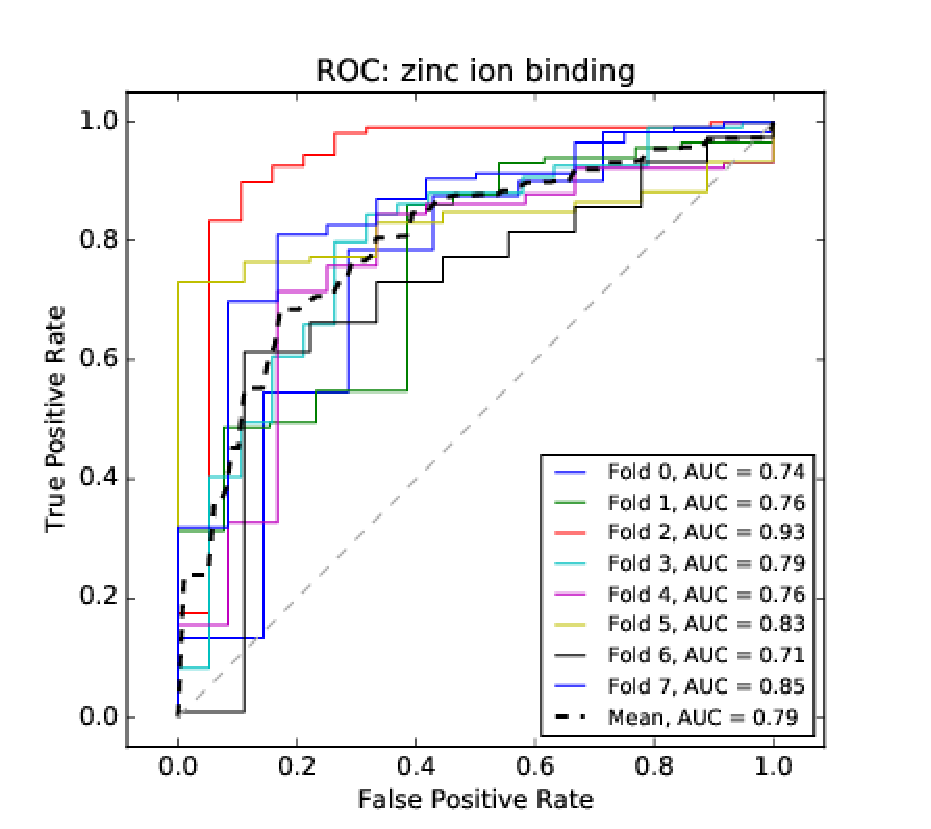
\includegraphics[width=\linewidth]{figures/roc_zinc_ion_binding}\captionof{figure}{Results for zinc ion binding}\label{fig:roc_zinc_ion_binding}\end{center}\end{Figure}
\begin{Figure}\begin{center}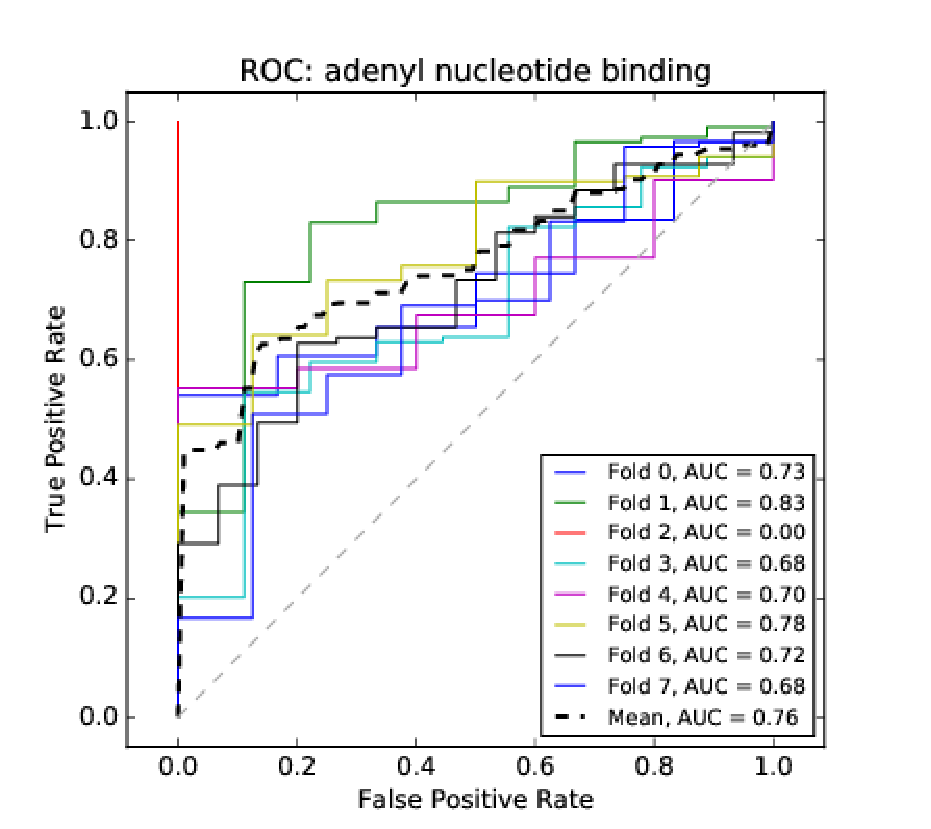
\includegraphics[width=\linewidth]{figures/roc_adenyl_nucleotide_binding}\captionof{figure}{Results for adenyl nucleotide binding}\label{fig:roc_adenyl_nucleotide_binding}\end{center}\end{Figure}
\begin{Figure}\begin{center}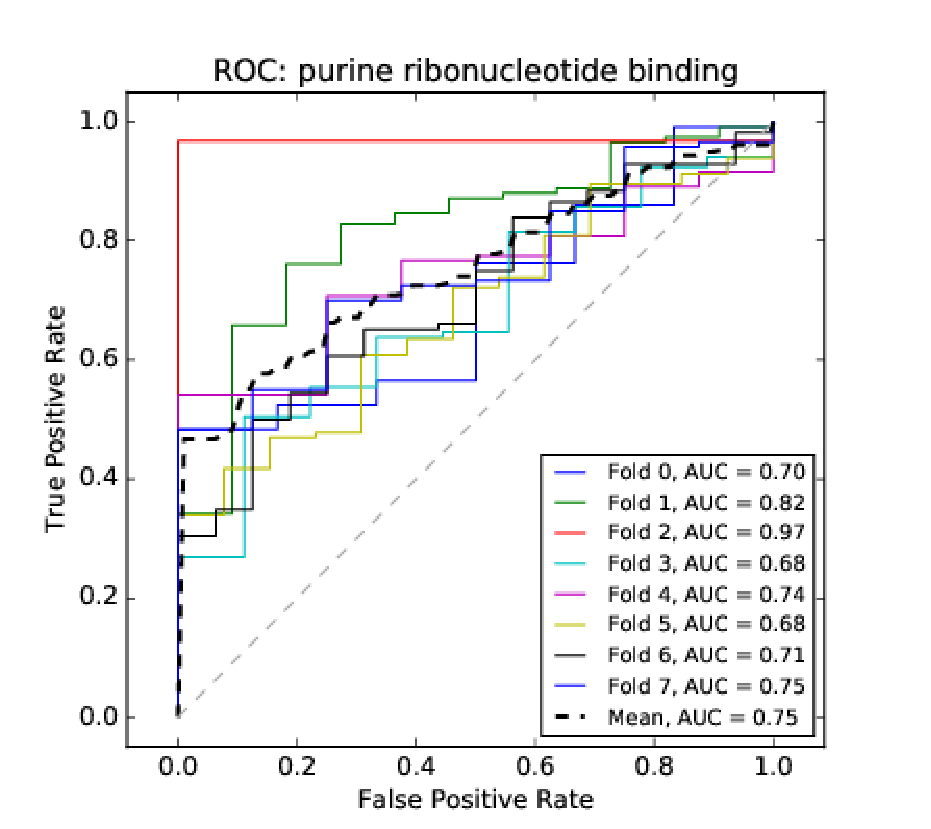
\includegraphics[width=\linewidth]{figures/roc_purine_ribonucleotide_binding}\captionof{figure}{Results for purine ribonucleotide binding}\label{fig:roc_purine_ribonucleotide_binding}\end{center}\end{Figure}
\begin{Figure}\begin{center}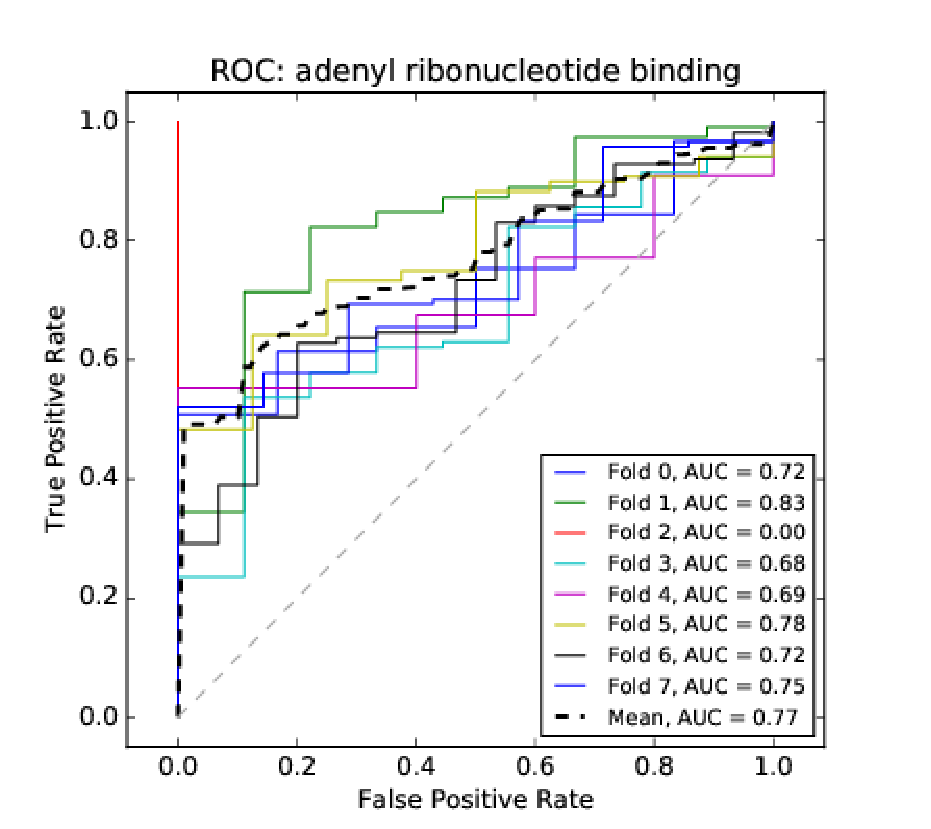
\includegraphics[width=\linewidth]{figures/roc_adenyl_ribonucleotide_binding}\captionof{figure}{Results for adenyl ribonucleotide binding}\label{fig:roc_adenyl_ribonucleotide_binding}\end{center}\end{Figure}
\end{multicols}

\section{Discovered structural patterns}
As mentioned earlier, the features generated by RelF represent certain structural patterns 
and the classifier training is basically deciding,
how much determining is the presence or absence of each of these patterns for the protein to exhibit certain function.
It is possible to evaluate, how much determining a certain pattern is,
in this work the information gain ratio criterion on training data was used to assess that.
The best performing patterns according to this criterion are summarized in tables \ref{tab:catalytic_activity}-\ref{tab:adenyl_ribonucleotide_binding}.
The number \textbf{N} is the number of cross-validation folds (out of 8) in which the given feature was found
among the top ten scoring.
For each function, all features that scored in top ten in at least 2 folds are included.

A very interesting property of this type of patterns is that they can
be interpreted in terms of molecular biology;
the patterns describe a certain local chemical configuration that could
be likely to be found in the protein's active site (ligand).
For example, notice how all of the structural patterns found for anion binding (Table \ref{tab:anion_binding})
require a polar amino acid residue present. 
That makes sense, the active site of the protein builds a magnetic field that can capture the ion.
Most (but not all) of the features for cation binding (Table \ref{tab:cation_binding})
also require a polar amino acid residue and we can further observe that except for RNA-binding the negatively charged
aspartic acid only appears in features for cation binding and it's subsets,
which is also does not contradict intuition. 

We can again compare these results to the results in \cite{szabova},
where discovered structural patterns for DNA-binding are described.
On the first sight, the patterns discovered here (Table \ref{tab:DNA_binding}) look different,
but that is mainly due the inclusion of polarity, charge and secondary structure information
and of course the described differences in data set construction.
Note also,  that the $\chi^2$ criterion was used in \cite{szabova}, not the information gain ratio.
However, we can confirm the importance of presence of the amino acids histidine
and cysteine in DNA-binding sites, which was presented in \cite{szabova}.
Because if focused on zinc-finger DNA-binding proteins, 
we can also have a look at discovered patterns for zinc ion binding (Table \ref{tab:zinc_ion_binding})
and observe that patterns containing the amino acids cysteine are again frequent there and phenylalanine,
found to be significant too in \cite{szabova} is also present.

Is is interesting to study how the discovered patterns for a given function
are often similar.
For example, in the patterns for zinc ion binding (Table \ref{tab:zinc_ion_binding}) all the top three patterns require a neutral amino acid residue
in the same distance to a cysteine residue while the secondary structure requirements are also similar.

A remarkable observation is the frequent presence of $3_{10}$-helices and $\beta$-bridges in the patterns,
despite being relatively rare type of secondary structure.
They cover only 3.48\% and 1.17\% of the overall secondary structure.
Yet, $3_{10}$-helices appear in 5 of 12 interesting features found for catalytic activity (Table \ref{tab:catalytic_activity}).
They are also frequent in
RNA binding (6 of 13, Table \ref{tab:RNA_binding}),
heterocyclic compound binding (6 of 13, Table \ref{tab:heterocyclic_compound_binding}),
organic cyclic compound binding (5 of 13, Table \ref{tab:organic_cyclic_compound_binding}),
ion binding (3 of 11, Table \ref{tab:ion_binding}),
hydrolase activity (3 of 12, Table \ref{tab:hydrolase_activity}),
metal ion binding (3 of 12, Table \ref{tab:metal_ion_binding}) 
and also appear less frequently in many other functions.
In the second case, $\beta$-bridges are frequent in features for 
zinc ion binding (6 of 15, Table \ref{tab:zinc_ion_binding}),
the more general function transition metal ion binding (6 of 18, Table \ref{tab:transition_metal_ion_binding}),
purine nucleoside binding (3 of 10, Table \ref{tab:purine_nucleoside_binding}),
receptor binding (3 of 17, Table \ref{tab:receptor_binding})
and less frequently also in features for other functions.
For comparison, table \ref{tab:secstr} displays the frequencies of secondary structure types in the data.
\begin{table}[h]\begin{center}\begin{tabular}{lrr}\textbf{Secondary structure type} & \textbf{\% of all data} & \textbf{\% of known} \\ \hline  
$\alpha$-helix & 31.07 & 41.42 \\ \hline
$\beta$-strand & 20.11 & 26.81 \\ \hline
Turn & 10.69 & 14.25 \\ \hline
Bend & 8.47 & 11.29 \\ \hline
$3_{10}$-helix & 3.48 & 4.64 \\ \hline
$\beta$-bridge & 1.17 & 1.57 \\ \hline
$\pi$-helix & 0.02 & 0.03 \\ \hline
Unknown (coil)  & 24.97 & - \\ \hline
\end{tabular}\end{center}\caption{Frequencies of secondary structure types}\label{tab:secstr}\end{table}
This prevalence of rare secondary structure types in 
structural patterns defining for functions
demands a~biolomolecular explanation
which the author of this work is currently unable to give
and a~possibility of further research is thus offered.

\begin{table}[h]\begin{tabularx}{\textwidth}{cX}\textbf{N} & \textbf{Feature} \\ \hline  
8 & Dist(A, B, 14),  Type(A, gly), Type(B, ile), SecStr(B, $3_{10}$-helix)\\ \hline 
7 & Dist(A, B, 14), Polar(C, yes),  Type(A, gly), Type(B, C), SecStr(A, $3_{10}$-helix), \newline SecStr(B, bend)\\ \hline 
7 & Dist(A, B, 14), Dist(A, C, 14),  Type(B, lys), SecStr(A, $\alpha$-helix), SecStr(C, $3_{10}$-helix)\\ \hline 
5 & Dist(A, B, 14), Polar(C, yes),  Type(A, met), Type(B, C), SecStr(A, bend), \newline SecStr(B, $3_{10}$-helix)\\ \hline 
5 & Dist(A, B, 10),  Type(A, pro), Type(B, lys)\\ \hline 
3 & Dist(A, B, 14),  Type(A, his), Type(B, gly), SecStr(A, $\beta$-strand), SecStr(B, bend)\\ \hline 
3 & Charge(D, -), Dist(A, B, 14), Polar(C, no),  Type(A, D), Type(B, C), SecStr(A, turn), SecStr(B, $\beta$-strand)\\ \hline 
2 & Dist(A, B, 14),  Type(B, phe), SecStr(A, turn), SecStr(B, $\beta$-bridge)\\ \hline 
2 & Dist(A, B, 14),  Type(B, lys), SecStr(A, $\alpha$-helix), SecStr(B, $3_{10}$-helix)\\ \hline 
2 & Dist(A, B, 14), Dist(A, C, 14), Polar(D, no),  Type(B, asp), Type(C, D), \newline SecStr(A, turn)\\ \hline 
2 & Charge(C, +), Dist(A, B, 10),  Type(B, C), SecStr(A, bend)\\ \hline 
2 & Charge(B, -), Dist(A, C, 14), Polar(D, no),  Type(A, B), Type(C, D), SecStr(A, turn), SecStr(C, $\beta$-strand)\\ \hline 
 \end{tabularx}\caption{Structural patterns for catalytic activity}\label{tab:catalytic_activity}\end{table}
\begin{table}\begin{tabularx}{\textwidth}{cX}\textbf{N} & \textbf{Feature} \\ \hline  
5 & Dist(A, B, 14),  Type(A, his), Type(B, arg), SecStr(A, $\beta$-strand), SecStr(B, $\beta$-strand)\\ \hline 
5 & Dist(A, B, 14),  Type(A, gln), Type(B, arg), SecStr(B, $\beta$-strand)\\ \hline 
4 & Dist(A, B, 14),  Type(A, his), Type(B, arg), SecStr(A, $\beta$-strand)\\ \hline 
4 & Dist(A, B, 14),  Type(A, ala), Type(B, ala), SecStr(A, $\beta$-strand), SecStr(B, $\beta$-strand)\\ \hline 
3 & Dist(A, B, 14),  Type(A, tyr), Type(B, ala), SecStr(B, $\beta$-strand)\\ \hline 
3 & Dist(A, B, 14),  Type(A, lys), Type(B, val), SecStr(A, turn)\\ \hline 
3 & Dist(A, B, 14),  Type(A, lys), Type(B, asp), SecStr(A, $3_{10}$-helix)\\ \hline 
3 & Dist(A, B, 14),  Type(A, ala), Type(B, trp), SecStr(A, $\alpha$-helix), SecStr(B, $\alpha$-helix)\\ \hline 
3 & Charge(C, 0), Dist(A, B, 14),  Type(A, tyr), Type(B, C), SecStr(A, $\alpha$-helix), \newline SecStr(B, turn)\\ \hline 
2 & Dist(A, C, 14), Dist(A, D, 14), Polar(B, no),  Type(A, B), Type(C, phe), \newline SecStr(A, bend), SecStr(D, turn)\\ \hline 
2 & Dist(A, B, 14),  Type(A, thr), Type(B, gln), SecStr(A, turn)\\ \hline 
2 & Dist(A, B, 14),  Type(A, phe), Type(B, leu), SecStr(A, bend)\\ \hline 
2 & Dist(A, B, 14),  Type(A, asp), Type(B, ile), SecStr(B, turn)\\ \hline 
2 & Dist(A, B, 14),  Type(A, arg), Type(B, trp), SecStr(A, $\beta$-strand), SecStr(B, $\beta$-strand)\\ \hline 
2 & Dist(A, B, 14),  Type(A, ala), Type(B, trp), SecStr(B, $\alpha$-helix)\\ \hline 
2 & Dist(A, B, 14), Polar(C, yes),  Type(A, tyr), Type(B, C), SecStr(A, $\beta$-bridge)\\ \hline 
2 & Charge(B, 0), Dist(A, C, 14), Polar(B, yes),  Type(A, B), Type(C, met), \newline SecStr(C, $\beta$-strand)\\ \hline 
 \end{tabularx}\caption{Structural patterns for binding}\label{tab:binding}\end{table}
\begin{table}\begin{tabularx}{\textwidth}{cX}\textbf{N} & \textbf{Feature} \\ \hline  
4 & Charge(D, 0), Charge(E, 0), Dist(A, B, 14), Dist(A, C, 14),  Type(A, E), \newline Type(B, leu), Type(C, D), SecStr(A, $\alpha$-helix), SecStr(C, $\alpha$-helix)\\ \hline 
3 & Dist(A, B, 14),  Type(A, leu), Type(B, leu), SecStr(B, $\alpha$-helix)\\ \hline 
3 & Charge(B, 0), Dist(A, C, 14),  Type(A, B), Type(C, leu), SecStr(A, $\alpha$-helix)\\ \hline 
2 & Dist(A, B, 14),  Type(A, ala), Type(B, lys), SecStr(A, $\alpha$-helix)\\ \hline 
2 & Dist(A, B, 14), Dist(A, D, 14), Polar(C, no),  Type(B, C), Type(D, leu), \newline SecStr(B, $\alpha$-helix)\\ \hline 
2 & Charge(C, 0), Dist(A, B, 14),  Type(A, C), Type(B, leu), SecStr(A, $\alpha$-helix)\\ \hline 
2 & Charge(C, 0), Dist(A, B, 14), Dist(A, D, 14), Polar(E, yes),  Type(A, leu), \newline Type(B, C), Type(D, E), SecStr(A, $\alpha$-helix)\\ \hline 
 \end{tabularx}\caption{Structural patterns for protein binding}\label{tab:protein_binding}\end{table}
\begin{table}\begin{tabularx}{\textwidth}{cX}\textbf{N} & \textbf{Feature} \\ \hline  
5 & Dist(A, B, 14),  Type(A, ser), Type(B, ile), SecStr(A, bend), SecStr(B, $\alpha$-helix)\\ \hline 
4 & Dist(A, B, 14),  Type(A, cys), SecStr(A, $\beta$-strand), SecStr(B, $\alpha$-helix)\\ \hline 
4 & Dist(A, B, 14), Dist(A, D, 14), Polar(C, no), Polar(E, yes),  Type(A, ala), \newline Type(B, C), Type(D, E), SecStr(D, turn)\\ \hline 
3 & Dist(A, B, 14),  Type(A, gly), Type(B, trp), SecStr(A, $3_{10}$-helix), SecStr(B, $3_{10}$-helix)\\ \hline 
3 & Dist(A, B, 14), Dist(A, C, 14),  Type(B, gln), Type(C, gly), SecStr(C, turn)\\ \hline 
2 & Dist(A, B, 14), Dist(A, D, 14), Polar(C, yes), Polar(E, no),  Type(A, ala), \newline Type(B, C), Type(D, E), SecStr(B, turn)\\ \hline 
2 & Dist(A, B, 14), Dist(A, C, 14),  Type(B, gly), Type(C, gln), SecStr(B, turn)\\ \hline 
2 & Dist(A, B, 14), Dist(A, C, 14), Polar(D, yes),  Type(C, D), SecStr(A, $\beta$-strand), \newline SecStr(B, turn), SecStr(C, $\beta$-strand)\\ \hline 
2 & Charge(F, 0), Dist(A, B, 14), Dist(A, C, 14), Dist(A, E, 14), Polar(D, yes),  \newline Type(B, gly), Type(C, D), Type(E, F), SecStr(C, turn), SecStr(E, turn)\\ \hline 
2 & Charge(B, -), Dist(A, C, 14), Dist(A, E, 14), Polar(D, yes),  Type(A, B), Type(C, D), Type(E, gly), SecStr(E, turn)\\ \hline 
 \end{tabularx}\caption{Structural patterns for transferase activity}\label{tab:transferase_activity}\end{table}
\begin{table}\begin{tabularx}{\textwidth}{cX}\textbf{N} & \textbf{Feature} \\ \hline  
7 & Charge(C, +), Dist(A, B, 14),  Type(A, ser), Type(B, C), SecStr(A, turn), \newline SecStr(B, $3_{10}$-helix)\\ \hline 
6 & Dist(A, B, 14),  Type(A, arg), Type(B, trp), SecStr(B, $\beta$-bridge)\\ \hline 
4 & Dist(A, B, 14),  Type(A, his), Type(B, gly), SecStr(A, bend)\\ \hline 
4 & Dist(A, B, 14),  Type(A, gln), Type(B, arg), SecStr(A, turn), SecStr(B, $\beta$-strand)\\ \hline 
4 & Dist(A, B, 14), Polar(C, no),  Type(A, asn), Type(B, C), SecStr(A, turn), \newline SecStr(B, turn)\\ \hline 
3 & Dist(A, B, 14), Dist(A, C, 14),  Type(B, ala), Type(C, pro)\\ \hline 
3 & Charge(E, -), Dist(A, B, 14), Dist(A, D, 14), Polar(C, no),  Type(A, gly), \newline Type(B, C), Type(D, E), SecStr(A, $\alpha$-helix)\\ \hline 
3 & Charge(B, -), Dist(A, C, 14),  Type(A, B), Type(C, glu), SecStr(A, bend), \newline SecStr(C, $3_{10}$-helix)\\ \hline 
2 & Dist(A, B, 14), Dist(A, C, 14),  Type(B, pro), Type(C, ala)\\ \hline 
2 & Charge(E, 0), Charge(F, 0), Dist(A, B, 14), Dist(A, D, 14), Polar(C, no), \newline Polar(E, yes),  Type(A, F), Type(B, C), Type(D, E), SecStr(A, $\alpha$-helix)\\ \hline 
2 & Charge(C, 0), Charge(E, +), Dist(A, B, 14), Dist(A, D, 14),  Type(A, gly), \newline Type(B, C), Type(D, E), SecStr(A, $3_{10}$-helix)\\ \hline 
2 & Charge(C, -), Charge(F, 0), Dist(A, B, 14), Dist(A, E, 14), Polar(D, yes),  \newline Type(A, D), Type(B, C), Type(E, F), SecStr(A, $\alpha$-helix)\\ \hline 
 \end{tabularx}\caption{Structural patterns for hydrolase activity}\label{tab:hydrolase_activity}\end{table}
\begin{table}\begin{tabularx}{\textwidth}{cX}\textbf{N} & \textbf{Feature} \\ \hline  
5 & Dist(A, B, 14),  Type(B, met), SecStr(A, $\beta$-strand), SecStr(B, $3_{10}$-helix)\\ \hline 
5 & Dist(A, B, 14),  Type(A, val), Type(B, ala), SecStr(A, $\alpha$-helix), SecStr(B, bend)\\ \hline 
5 & Dist(A, B, 14), Dist(A, C, 14), Polar(D, yes),  Type(C, D), SecStr(A, $\beta$-strand), \newline SecStr(B, turn), SecStr(C, $\beta$-strand)\\ \hline 
4 & Dist(A, B, 14),  Type(A, ser), Type(B, phe), SecStr(A, $3_{10}$-helix), SecStr(B, $\alpha$-helix)\\ \hline 
4 & Dist(A, B, 14),  Type(A, phe), Type(B, leu), SecStr(A, turn), SecStr(B, $\beta$-strand)\\ \hline 
4 & Charge(C, +), Dist(A, B, 14), Dist(A, D, 14), Polar(E, no),  Type(B, C), \newline Type(D, E), SecStr(B, turn), SecStr(D, turn)\\ \hline 
4 & Charge(C, +), Charge(E, -), Dist(A, B, 14), Dist(A, D, 12),  Type(B, C), Type(D, E)\\ \hline 
3 & Charge(C, +), Dist(A, B, 14),  Type(A, C), Type(B, leu), SecStr(A, $\beta$-strand), \newline SecStr(B, $\beta$-bridge)\\ \hline 
3 & Charge(C, 0), Dist(A, B, 14), Dist(A, D, 14), Polar(C, yes), Polar(E, no),  \newline Type(B, C), Type(D, E), SecStr(A, $\beta$-strand), SecStr(D, turn)\\ \hline 
3 & Charge(B, +), Dist(A, C, 14),  Type(A, B), Type(C, leu), SecStr(A, $\beta$-strand), \newline SecStr(C, $\beta$-bridge)\\ \hline 
2 & Charge(E, +), Dist(A, B, 14), Dist(A, D, 14), Polar(C, no),  Type(B, C), \newline Type(D, E), SecStr(B, turn), SecStr(D, turn)\\ \hline 
 \end{tabularx}\caption{Structural patterns for small molecule binding}\label{tab:small_molecule_binding}\end{table}
\begin{table}\begin{tabularx}{\textwidth}{cX}\textbf{N} & \textbf{Feature} \\ \hline  
7 & Dist(A, B, 14), Polar(C, yes),  Type(A, gln), Type(B, C), SecStr(A, $3_{10}$-helix), \newline SecStr(B, $\alpha$-helix)\\ \hline 
6 & Dist(A, B, 14),  Type(A, lys), Type(B, gln), SecStr(A, $\alpha$-helix), SecStr(B, bend)\\ \hline 
6 & Dist(A, B, 14),  Type(A, gly), Type(B, asn), SecStr(A, bend), SecStr(B, $\beta$-strand)\\ \hline 
5 & Dist(A, B, 14), Polar(C, yes),  Type(A, C), Type(B, his), SecStr(A, $3_{10}$-helix), \newline SecStr(B, $\alpha$-helix)\\ \hline 
4 & Dist(A, C, 14), Polar(B, no),  Type(A, B), Type(C, ser), SecStr(A, $\alpha$-helix), \newline SecStr(C, bend)\\ \hline 
3 & Dist(A, B, 14), Polar(C, no),  Type(A, arg), Type(B, C), SecStr(A, $\alpha$-helix), \newline SecStr(B, $\beta$-strand)\\ \hline 
2 & Dist(A, C, 14), Polar(B, yes),  Type(A, B), Type(C, his), SecStr(A, $3_{10}$-helix), \newline SecStr(C, $\alpha$-helix)\\ \hline 
2 & Dist(A, B, 14),  Type(A, leu), Type(B, cys), SecStr(A, turn), SecStr(B, $\beta$-strand)\\ \hline 
2 & Dist(A, B, 14),  Type(A, glu), Type(B, arg), SecStr(A, $\beta$-bridge)\\ \hline 
2 & Dist(A, B, 14), Polar(C, no),  Type(A, C), Type(B, ser), SecStr(A, $\alpha$-helix), \newline SecStr(B, bend)\\ \hline 
2 & Dist(A, B, 14), Polar(C, no),  Type(A, C), Type(B, ile), SecStr(B, $\beta$-bridge)\\ \hline 
 \end{tabularx}\caption{Structural patterns for ion binding}\label{tab:ion_binding}\end{table}
\begin{table}\begin{tabularx}{\textwidth}{cX}\textbf{N} & \textbf{Feature} \\ \hline  
8 & Dist(A, B, 14),  Type(A, tyr), Type(B, met), SecStr(A, bend)\\ \hline 
6 & Dist(A, B, 14), Dist(A, C, 14),  Type(A, gly), Type(B, phe), SecStr(A, bend), \newline SecStr(C, $3_{10}$-helix)\\ \hline 
6 & Charge(C, 0), Dist(A, B, 14), Polar(C, yes),  Type(A, gln), Type(B, C), \newline SecStr(A, $3_{10}$-helix), SecStr(B, $\alpha$-helix)\\ \hline 
5 & Dist(A, B, 14),  Type(A, gly), Type(B, phe), SecStr(A, bend), SecStr(B, $3_{10}$-helix)\\ \hline 
5 & Charge(B, 0), Dist(A, C, 12), Polar(B, yes),   Type(A, B), SecStr(A, bend)\\ \hline 
4 & Dist(A, B, 14),  Type(A, gln), Type(B, his), SecStr(A, $3_{10}$-helix), SecStr(B, $\alpha$-helix)\\ \hline 
3 & Charge(C, 0), Dist(A, B, 14), Dist(A, D, 12),   Type(A, arg), Type(B, C)\\ \hline 
3 & Charge(B, +), Dist(A, C, 14),  Type(A, B), Type(C, leu), SecStr(A, $3_{10}$-helix)\\ \hline 
2 & Dist(A, B, 14), Polar(C, no),  Type(A, val), Type(B, C), SecStr(A, $\beta$-strand), \newline SecStr(B, $\beta$-bridge)\\ \hline 
2 & Dist(A, B, 14), Dist(A, D, 14), Polar(C, yes),  Type(A, C), Type(D, arg), \newline SecStr(B, turn)\\ \hline 
2 & Dist(A, B, 14), Dist(A, D, 12), Polar(C, no), Polar(E, yes),   Type(A, E), Type(B, C), SecStr(A, bend)\\ \hline 
2 & Charge(D, 0), Dist(A, C, 12), Dist(A, E, 14), Polar(B, yes),   Type(A, B), \newline Type(C, D), SecStr(A, bend)\\ \hline 
2 & Charge(C, 0), Charge(E, 0), Dist(A, B, 14), Dist(A, D, 12), Polar(F, yes),  \newline Type(A, F), Type(B, C), Type(D, E), SecStr(A, bend)\\ \hline 
 \end{tabularx}\caption{Structural patterns for organic cyclic compound binding}\label{tab:organic_cyclic_compound_binding}\end{table}
\begin{table}\begin{tabularx}{\textwidth}{cX}\textbf{N} & \textbf{Feature} \\ \hline  
5 & Dist(A, B, 14),  Type(A, lys), Type(B, glu), SecStr(B, turn)\\ \hline 
5 & Charge(C, +), Dist(A, B, 14), Dist(A, D, 14), Polar(E, no),  Type(B, C), \newline Type(D, E), SecStr(B, turn), SecStr(D, turn)\\ \hline 
4 & Dist(A, B, 8),  Type(B, val), SecStr(A, bend), SecStr(B, $\beta$-strand)\\ \hline 
4 & Dist(A, B, 14),  Type(A, leu), Type(B, gly), SecStr(A, $\alpha$-helix), SecStr(B, $\beta$-strand)\\ \hline 
4 & Dist(A, B, 10), Polar(C, yes),  Type(A, ala), Type(B, C), SecStr(A, $\alpha$-helix)\\ \hline 
3 & Dist(A, C, 10), Polar(B, no),  Type(A, B), Type(C, thr), SecStr(A, bend)\\ \hline 
3 & Charge(C, 0), Charge(D, 0), Dist(A, B, 14), Polar(D, yes),  Type(A, D), Type(B, C), SecStr(A, $\beta$-strand), SecStr(B, turn)\\ \hline 
3 & Charge(C, -), Dist(A, B, 14),  Type(A, C), SecStr(A, $\beta$-strand), SecStr(B, $\beta$-bridge)\\ \hline 
3 & Charge(B, 0), Charge(D, 0), Dist(A, C, 14), Polar(B, yes),  Type(A, B), Type(C, D), SecStr(A, $\beta$-strand), SecStr(C, turn)\\ \hline 
2 & Dist(A, B, 14),  Type(A, thr), Type(B, thr), SecStr(A, $\beta$-strand), SecStr(B, $\beta$-strand)\\ \hline 
2 & Dist(A, B, 14), Dist(A, C, 14), Dist(A, D, 14),  Type(D, lys), SecStr(A, bend),  \newline SecStr(B, turn), SecStr(C, bend)\\ \hline 
2 & Charge(E, +), Dist(A, B, 14), Dist(A, D, 14), Polar(C, no),  Type(B, C),  \newline Type(D, E), SecStr(B, turn), SecStr(D, turn)\\ \hline 
2 & Charge(C, 0), Dist(A, B, 14), Dist(A, E, 14), Polar(C, yes), Polar(D, no), \newline Polar(F, no),  Type(A, D), Type(B, C), Type(E, F), SecStr(A, $\beta$-strand), SecStr(E, turn)\\ \hline 
2 & Charge(B, -), Dist(A, C, 14),  Type(A, B), SecStr(A, $\beta$-strand), SecStr(C, $\beta$-bridge)\\ \hline 
 \end{tabularx}\caption{Structural patterns for carbohydrate derivative binding}\label{tab:carbohydrate_derivative_binding}\end{table}
\begin{table}\begin{tabularx}{\textwidth}{cX}\textbf{N} & \textbf{Feature} \\ \hline  
8 & Dist(A, B, 14),  Type(A, tyr), Type(B, met), SecStr(A, bend)\\ \hline 
7 & Charge(C, 0), Dist(A, B, 14), Polar(C, yes),  Type(A, gln), Type(B, C), \newline SecStr(A, $3_{10}$-helix), SecStr(B, $\alpha$-helix)\\ \hline 
5 & Dist(A, B, 14),  Type(A, gly), Type(B, phe), SecStr(A, bend), SecStr(B, $3_{10}$-helix)\\ \hline 
4 & Dist(A, B, 14), Polar(C, no),  Type(A, val), Type(B, C), SecStr(A, $\beta$-strand), \newline SecStr(B, $\beta$-bridge)\\ \hline 
4 & Dist(A, B, 14), Dist(A, C, 14),  Type(A, gly), Type(B, phe), SecStr(A, bend), \newline SecStr(C, $3_{10}$-helix)\\ \hline 
3 & Dist(A, B, 14),  Type(A, gln), Type(B, his), SecStr(A, $3_{10}$-helix), SecStr(B, $\alpha$-helix)\\ \hline 
3 & Charge(D, 0), Dist(A, B, 12), Dist(A, C, 14),   Type(A, arg), Type(C, D)\\ \hline 
3 & Charge(C, 0), Dist(A, B, 12), Polar(C, yes),   Type(A, C), SecStr(A, bend)\\ \hline 
3 & Charge(B, 0), Dist(A, C, 12), Polar(B, yes),   Type(A, B), SecStr(A, bend)\\ \hline 
2 & Dist(A, B, 14), Dist(A, C, 14),  Type(A, gly), Type(C, phe), SecStr(A, bend), \newline SecStr(B, $3_{10}$-helix)\\ \hline 
2 & Dist(A, B, 12), Dist(A, C, 14), Polar(D, no), Polar(E, yes),   Type(A, E), Type(C, D), SecStr(A, bend)\\ \hline 
2 & Charge(C, 0), Dist(A, B, 12), Dist(A, E, 14), Polar(D, yes),   Type(A, D), \newline Type(B, C), SecStr(A, bend)\\ \hline 
2 & Charge(B, +), Dist(A, C, 14),  Type(A, B), Type(C, leu), SecStr(A, $3_{10}$-helix)\\ \hline 
 \end{tabularx}\caption{Structural patterns for heterocyclic compound binding}\label{tab:heterocyclic_compound_binding}\end{table}
\begin{table}\begin{tabularx}{\textwidth}{cX}\textbf{N} & \textbf{Feature} \\ \hline  
5 & Dist(A, B, 14),  Type(A, lys), Type(B, glu), SecStr(B, turn)\\ \hline 
5 & Dist(A, B, 14),  Type(A, leu), Type(B, gly), SecStr(A, $\alpha$-helix), SecStr(B, $\beta$-strand)\\ \hline 
5 & Dist(A, B, 10), Polar(C, no),  Type(A, C), Type(B, thr), SecStr(A, bend)\\ \hline 
3 & Dist(A, B, 14), Dist(A, C, 14), Polar(D, yes),  Type(A, gly), Type(B, met),  \newline Type(C, D)\\ \hline 
3 & Dist(A, B, 10), Polar(C, yes),  Type(A, ala), Type(B, C), SecStr(A, $\alpha$-helix)\\ \hline 
3 & Charge(D, +), Dist(A, C, 14), Dist(A, E, 14), Polar(B, no), Polar(F, no),  \newline Type(A, B), Type(C, D), Type(E, F), SecStr(C, turn), SecStr(E, turn)\\ \hline 
2 & Dist(A, B, 14),  Type(A, phe), Type(B, leu), SecStr(A, $3_{10}$-helix), SecStr(B, $3_{10}$-helix)\\ \hline 
2 & Dist(A, B, 14), Dist(A, D, 14), Polar(C, yes),  Type(A, gly), Type(B, C), \newline Type(D, met)\\ \hline 
2 & Charge(E, 0), Dist(A, B, 14), Dist(A, D, 14), Polar(C, no), Polar(E, yes), \newline Polar(F, no),  Type(A, F), Type(B, C), Type(D, E), SecStr(A, $\beta$-strand), \newline SecStr(B, turn)\\ \hline 
 \end{tabularx}\caption{Structural patterns for nucleoside binding}\label{tab:nucleoside_binding}\end{table}
\begin{table}\begin{tabularx}{\textwidth}{cX}\textbf{N} & \textbf{Feature} \\ \hline  
7 & Charge(C, 0), Dist(A, B, 14), Polar(C, yes),  Type(A, gln), Type(B, C), \newline SecStr(A, $3_{10}$-helix), SecStr(B, $\alpha$-helix)\\ \hline 
6 & Charge(C, +), Dist(A, B, 14),  Type(A, arg), Type(B, C), SecStr(A, $\alpha$-helix), \newline SecStr(B, bend)\\ \hline 
4 & Charge(C, 0), Dist(A, B, 14), Dist(A, D, 12),   Type(A, arg), Type(B, C)\\ \hline 
3 & Charge(C, +), Dist(A, B, 14),  Type(A, ile), Type(B, C), SecStr(A, bend), \newline SecStr(B, $\alpha$-helix)\\ \hline 
3 & Charge(C, 0), Dist(A, B, 14),  Type(A, gln), Type(B, C), SecStr(B, bend)\\ \hline 
3 & Charge(B, 0), Dist(A, C, 14), Polar(B, yes),  Type(A, B), Type(C, his), \newline SecStr(C, $3_{10}$-helix)\\ \hline 
2 & Dist(A, C, 14), Polar(B, yes),  Type(A, B), Type(C, lys), SecStr(A, $\beta$-strand), \newline SecStr(C, bend)\\ \hline 
2 & Dist(A, B, 14),  Type(A, glu), Type(B, pro), SecStr(A, bend), SecStr(B, bend)\\ \hline 
2 & Dist(A, B, 14), Polar(C, no),  Type(A, C), Type(B, asn), SecStr(A, $\beta$-bridge), \newline SecStr(B, $\beta$-strand)\\ \hline 
2 & Charge(D, 0), Dist(A, B, 12), Dist(A, C, 14),   Type(A, arg), Type(C, D)\\ \hline 
 \end{tabularx}\caption{Structural patterns for nucleic acid binding}\label{tab:nucleic_acid_binding}\end{table}
\begin{table}\begin{tabularx}{\textwidth}{cX}\textbf{N} & \textbf{Feature} \\ \hline  
7 & Dist(A, B, 14), Polar(C, yes),  Type(A, asn), Type(B, C), SecStr(A, turn), \newline SecStr(B, $\beta$-strand)\\ \hline 
6 & Dist(A, B, 14),  Type(A, lys), Type(B, leu), SecStr(A, turn), SecStr(B, $\beta$-bridge)\\ \hline 
5 & Dist(A, B, 14),  Type(A, pro), Type(B, glu)\\ \hline 
5 & Dist(A, B, 14),  Type(A, asp), Type(B, thr), SecStr(A, $\beta$-bridge), SecStr(B, bend)\\ \hline 
4 & Dist(A, B, 14),  Type(A, tyr), SecStr(A, $\beta$-bridge), SecStr(B, $\alpha$-helix)\\ \hline 
4 & Charge(B, 0), Charge(D, 0), Dist(A, C, 10), Polar(B, yes), Polar(D, yes),  \newline Type(A, B), Type(C, D), SecStr(A, bend)\\ \hline 
3 & Dist(A, B, 14), Dist(A, C, 14),  Type(C, ala), SecStr(B, bend), SecStr(C, $\alpha$-helix)\\ \hline 
3 & Dist(A, B, 14), Dist(A, C, 14),  Type(B, gln), Type(C, lys), SecStr(B, bend)\\ \hline 
3 & Dist(A, B, 14), Dist(A, C, 14),  Type(B, ala), SecStr(B, $\alpha$-helix), SecStr(C, bend)\\ \hline 
3 & Charge(E, 0), Dist(A, B, 14), Dist(A, D, 14), Polar(C, yes), Polar(E, yes),  \newline Type(B, C), Type(D, E), SecStr(A, bend), SecStr(B, bend), SecStr(D, turn)\\ \hline 
2 & Dist(A, B, 8),  Type(A, ser), Type(B, gly), SecStr(A, bend)\\ \hline 
2 & Dist(A, B, 14), Dist(A, D, 14), Polar(C, yes),  Type(A, C), Type(B, asn), \newline Type(D, glu)\\ \hline 
2 & Dist(A, B, 14), Dist(A, C, 14),  Type(B, lys), Type(C, gln), SecStr(C, bend)\\ \hline 
2 & Dist(A, B, 14), Dist(A, C, 14), Dist(A, E, 14), Polar(D, no),  Type(B, ile), \newline Type(C, D), Type(E, ala), SecStr(C, $\beta$-bridge)\\ \hline 
2 & Dist(A, B, 10),  Type(A, lys), Type(B, gly)\\ \hline 
2 & Charge(C, 0), Dist(A, B, 14), Dist(A, D, 14), Polar(C, yes), Polar(E, no),  \newline Type(B, C), Type(D, E), SecStr(A, bend), SecStr(B, turn)\\ \hline 
2 & Charge(C, 0), Charge(D, 0), Dist(A, B, 10), Polar(C, yes), Polar(D, yes),  \newline Type(A, D), Type(B, C), SecStr(A, bend)\\ \hline 
 \end{tabularx}\caption{Structural patterns for receptor binding}\label{tab:receptor_binding}\end{table}
\begin{table}\begin{tabularx}{\textwidth}{cX}\textbf{N} & \textbf{Feature} \\ \hline  
5 & Dist(A, B, 14), Dist(A, C, 14), Polar(D, yes),  Type(C, D), SecStr(A, $\beta$-strand), \newline SecStr(B, turn), SecStr(C, $\beta$-strand)\\ \hline 
4 & Charge(E, 0), Dist(A, B, 14), Dist(A, D, 14), Polar(C, no), Polar(E, yes),  \newline Type(B, C), Type(D, E), SecStr(A, $\beta$-strand), SecStr(B, turn)\\ \hline 
4 & Charge(C, 0), Charge(D, 0), Dist(A, B, 14), Polar(D, yes),  Type(A, D), Type(B, C), SecStr(A, $\beta$-strand), SecStr(B, turn)\\ \hline 
3 & Dist(A, B, 14),  Type(A, thr), Type(B, ser), SecStr(A, turn), SecStr(B, $3_{10}$-helix)\\ \hline 
3 & Dist(A, B, 14),  Type(A, ile), Type(B, his), SecStr(A, $\beta$-bridge), SecStr(B, turn)\\ \hline 
2 & Dist(A, B, 14),  Type(A, lys), Type(B, glu), SecStr(B, turn)\\ \hline 
2 & Charge(C, +), Dist(A, B, 14),  Type(A, C), Type(B, tyr), SecStr(A, $\alpha$-helix),  \newline SecStr(B, $\beta$-strand)\\ \hline 
2 & Charge(C, 0), Dist(A, B, 14), Dist(A, D, 14), Polar(C, yes), Polar(E, no),  \newline Type(B, C), Type(D, E), SecStr(A, $\beta$-strand), SecStr(D, turn)\\ \hline 
2 & Charge(B, 0), Charge(D, 0), Dist(A, C, 14), Polar(B, yes),  Type(A, B), Type(C, D), SecStr(A, $\beta$-strand), SecStr(C, turn)\\ \hline 
 \end{tabularx}\caption{Structural patterns for anion binding}\label{tab:anion_binding}\end{table}
\begin{table}\begin{tabularx}{\textwidth}{cX}\textbf{N} & \textbf{Feature} \\ \hline  
7 & Charge(C, 0), Dist(A, B, 14), Polar(C, yes),  Type(A, gln), Type(B, C), \newline  SecStr(A, $3_{10}$-helix), SecStr(B, $\alpha$-helix)\\ \hline 
3 & Charge(C, +), Dist(A, B, 14),  Type(A, C), Type(B, ile), SecStr(A, $\beta$-bridge), \newline SecStr(B, bend)\\ \hline 
2 & Dist(A, B, 14),  Type(A, tyr), Type(B, cys), SecStr(A, turn), SecStr(B, $\beta$-strand)\\ \hline 
2 & Dist(A, B, 14),  Type(A, phe), Type(B, tyr), SecStr(A, $\beta$-bridge), SecStr(B, bend)\\ \hline 
2 & Dist(A, B, 14),  Type(A, phe), Type(B, cys), SecStr(A, bend), SecStr(B, turn)\\ \hline 
2 & Dist(A, B, 14), Dist(A, E, 14), Polar(C, yes), Polar(D, no),  Type(A, D), Type(B, C), Type(E, gly), SecStr(A, $\alpha$-helix), SecStr(E, turn)\\ \hline 
2 & Charge(C, 0), Dist(A, B, 14), Polar(C, yes),  Type(A, thr), Type(B, C), \newline SecStr(A, bend), SecStr(B, turn)\\ \hline 
2 & Charge(C, 0), Dist(A, B, 14), Polar(C, yes),  Type(A, C), Type(B, cys), \newline SecStr(A, $\alpha$-helix), SecStr(B, $\beta$-strand)\\ \hline 
2 & Charge(C, 0), Dist(A, B, 14), Polar(C, yes),  Type(A, asp), Type(B, C), \newline SecStr(B, turn)\\ \hline 
2 & Charge(C, -), Dist(A, B, 14),  Type(A, C), Type(B, ala), SecStr(A, turn), \newline SecStr(B, $\alpha$-helix)\\ \hline 
2 & Charge(B, +), Dist(A, C, 14),  Type(A, B), Type(C, asn), SecStr(A, $3_{10}$-helix), \newline SecStr(C, turn)\\ \hline 
2 & Charge(B, 0), Dist(A, C, 14), Polar(B, yes),  Type(A, B), Type(C, cys), \newline SecStr(A, $\alpha$-helix), SecStr(C, $\beta$-strand)\\ \hline 
 \end{tabularx}\caption{Structural patterns for cation binding}\label{tab:cation_binding}\end{table}
\begin{table}\begin{tabularx}{\textwidth}{cX}\textbf{N} & \textbf{Feature} \\ \hline  
5 & Dist(A, B, 14),  Type(A, ser), Type(B, phe), SecStr(A, $3_{10}$-helix), SecStr(B, $\alpha$-helix)\\ \hline 
4 & Dist(A, B, 14),  Type(A, phe), Type(B, leu), SecStr(A, turn), SecStr(B, $\beta$-strand)\\ \hline 
3 & Dist(A, B, 14),  Type(A, gly), Type(B, tyr), SecStr(B, $\alpha$-helix)\\ \hline 
3 & Charge(C, +), Dist(A, B, 14),  Type(A, C), Type(B, leu), SecStr(A, $\beta$-strand), \newline SecStr(B, $\beta$-bridge)\\ \hline 
3 & Charge(C, 0), Dist(A, B, 14), Dist(A, D, 14),  Type(A, leu), Type(B, C), \newline Type(D, glu)\\ \hline 
3 & Charge(B, +), Dist(A, C, 14),  Type(A, B), Type(C, leu), SecStr(A, $\beta$-strand), \newline SecStr(C, $\beta$-bridge)\\ \hline 
2 & Dist(A, B, 14),  Type(A, leu), Type(B, gly), SecStr(A, $\alpha$-helix), SecStr(B, $\beta$-strand)\\ \hline 
2 & Dist(A, B, 14), Dist(A, C, 14), Polar(D, no),  Type(B, lys), Type(C, D), \newline SecStr(B, turn), SecStr(C, turn)\\ \hline 
 \end{tabularx}\caption{Structural patterns for nucleoside phosphate binding}\label{tab:nucleoside_phosphate_binding}\end{table}
\begin{table}\begin{tabularx}{\textwidth}{cX}\textbf{N} & \textbf{Feature} \\ \hline  
5 & Dist(A, B, 14),  Type(A, ser), Type(B, phe), SecStr(A, $3_{10}$-helix), SecStr(B, $\alpha$-helix)\\ \hline 
4 & Dist(A, B, 14),  Type(A, phe), Type(B, leu), SecStr(A, turn), SecStr(B, $\beta$-strand)\\ \hline 
3 & Dist(A, B, 14),  Type(A, gly), Type(B, tyr), SecStr(B, $\alpha$-helix)\\ \hline 
3 & Charge(C, +), Dist(A, B, 14),  Type(A, C), Type(B, leu), SecStr(A, $\beta$-strand), \newline SecStr(B, $\beta$-bridge)\\ \hline 
3 & Charge(C, 0), Dist(A, B, 14), Dist(A, D, 14),  Type(A, leu), Type(B, C), \newline Type(D, glu)\\ \hline 
3 & Charge(B, +), Dist(A, C, 14),  Type(A, B), Type(C, leu), SecStr(A, $\beta$-strand), \newline SecStr(C, $\beta$-bridge)\\ \hline 
2 & Dist(A, B, 14),  Type(A, leu), Type(B, gly), SecStr(A, $\alpha$-helix), SecStr(B, $\beta$-strand)\\ \hline 
2 & Dist(A, B, 14), Dist(A, C, 14), Polar(D, no),  Type(B, lys), Type(C, D), \newline SecStr(B, turn), SecStr(C, turn)\\ \hline 
 \end{tabularx}\caption{Structural patterns for nucleotide binding}\label{tab:nucleotide_binding}\end{table}
\begin{table}\begin{tabularx}{\textwidth}{cX}\textbf{N} & \textbf{Feature} \\ \hline  
5 & Dist(A, B, 14),  Type(A, lys), Type(B, glu), SecStr(B, turn)\\ \hline 
5 & Dist(A, B, 14),  Type(A, leu), Type(B, gly), SecStr(A, $\alpha$-helix), SecStr(B, $\beta$-strand)\\ \hline 
5 & Dist(A, B, 14), Dist(A, C, 14), Polar(D, yes),  Type(A, gly), Type(B, met), \newline Type(C, D)\\ \hline 
4 & Dist(A, B, 10), Polar(C, yes),  Type(A, ala), Type(B, C), SecStr(A, $\alpha$-helix)\\ \hline 
4 & Dist(A, B, 10), Polar(C, no),  Type(A, C), Type(B, thr), SecStr(A, bend)\\ \hline 
2 & Dist(A, B, 14),  Type(A, ile), Type(B, ser), SecStr(A, $\beta$-bridge), SecStr(B, turn)\\ \hline 
2 & Dist(A, B, 14),  Type(A, cys), Type(B, glu), SecStr(A, $\beta$-bridge), SecStr(B, turn)\\ \hline 
2 & Dist(A, B, 14),  Type(A, ala), Type(B, val), SecStr(A, $3_{10}$-helix), SecStr(B, $\beta$-strand)\\ \hline 
2 & Dist(A, B, 14),   Type(A, cys), SecStr(A, $\beta$-bridge)\\ \hline 
2 & Charge(F, 0), Dist(A, C, 14), Dist(A, E, 14), Polar(B, no), Polar(D, no), \newline Polar(F, yes),  Type(A, B), Type(C, D), Type(E, F), SecStr(A, $\beta$-strand), \newline SecStr(C, turn)\\ \hline 
 \end{tabularx}\caption{Structural patterns for purine nucleoside binding}\label{tab:purine_nucleoside_binding}\end{table}
\begin{table}\begin{tabularx}{\textwidth}{cX}\textbf{N} & \textbf{Feature} \\ \hline  
7 & Dist(A, B, 14),  Type(A, glu), Type(B, pro), SecStr(A, bend), SecStr(B, bend)\\ \hline 
6 & Dist(A, B, 14), Polar(C, no),  Type(A, glu), Type(B, C), SecStr(A, bend), \newline SecStr(B, bend)\\ \hline 
5 & Dist(A, B, 14),  Type(A, tyr), Type(B, his), SecStr(A, turn), SecStr(B, $\beta$-strand)\\ \hline 
5 & Dist(A, B, 14), Polar(C, no),  Type(A, met), Type(B, C), SecStr(B, bend)\\ \hline 
4 & Dist(A, B, 14),  Type(A, pro), SecStr(A, $\beta$-bridge), SecStr(B, $\beta$-bridge)\\ \hline 
3 & Dist(A, B, 14), Dist(A, C, 14), Polar(D, no),  Type(B, thr), Type(C, D), \newline SecStr(B, turn)\\ \hline 
2 & Dist(A, B, 14),  Type(B, cys), SecStr(A, $\alpha$-helix), SecStr(B, bend)\\ \hline 
2 & Charge(C, 0), Dist(A, B, 14),  Type(A, gln), Type(B, C), SecStr(B, bend)\\ \hline 
2 & Charge(B, 0), Charge(H, 0), Dist(A, C, 14), Dist(A, E, 14), Dist(A, G, 14), \newline Polar(D, no), Polar(F, yes),  Type(A, B), Type(C, D), Type(E, F), Type(G, H), \newline SecStr(A, turn), SecStr(G, turn)\\ \hline 
 \end{tabularx}\caption{Structural patterns for DNA binding}\label{tab:DNA_binding}\end{table}
\begin{table}\begin{tabularx}{\textwidth}{cX}\textbf{N} & \textbf{Feature} \\ \hline  
8 & Charge(C, +), Dist(A, B, 14),  Type(A, ile), Type(B, C), SecStr(A, bend), \newline SecStr(B, $\alpha$-helix)\\ \hline 
7 & Charge(C, 0), Dist(A, B, 14),  Type(A, his), Type(B, C), SecStr(B, $3_{10}$-helix)\\ \hline 
5 & Dist(A, B, 14),  Type(A, asp), Type(B, phe), SecStr(A, $3_{10}$-helix), SecStr(B, turn)\\ \hline 
4 & Dist(A, B, 14), Polar(C, no),  Type(A, lys), Type(B, C), SecStr(A, $3_{10}$-helix), \newline SecStr(B, $\beta$-strand)\\ \hline 
4 & Charge(C, 0), Dist(A, B, 14), Polar(C, yes),  Type(A, C), Type(B, his), \newline SecStr(B, $3_{10}$-helix)\\ \hline 
4 & Charge(B, 0), Dist(A, C, 14), Polar(B, yes),  Type(A, B), Type(C, his), \newline SecStr(C, $3_{10}$-helix)\\ \hline 
3 & Dist(A, B, 14), Polar(C, yes),  Type(A, pro), Type(B, C), SecStr(B, $3_{10}$-helix)\\ \hline 
3 & Dist(A, B, 14), Dist(A, D, 14), Polar(C, no), Polar(E, no),  Type(A, C), Type(B, ser), Type(D, E)\\ \hline 
3 & Charge(D, +), Dist(A, B, 8), Polar(C, no),  Type(A, D), Type(B, C), SecStr(A, bend)\\ \hline 
3 & Charge(B, +), Dist(A, C, 8), Polar(D, no),  Type(A, B), Type(C, D), SecStr(A, bend)\\ \hline 
2 & Dist(A, B, 8),  Type(A, gly), Type(B, pro), SecStr(B, turn)\\ \hline 
2 & Charge(D, 0), Dist(A, B, 14), Dist(A, C, 12),  Type(C, D), SecStr(A, turn), \newline SecStr(B, turn), SecStr(C, turn)\\ \hline 
2 & Charge(C, 0), Dist(A, B, 14), Dist(A, D, 14),  Type(A, C), Type(B, ser), \newline Type(D, leu)\\ \hline 
2 & Charge(C, 0), Dist(A, B, 12), Dist(A, D, 14),  Type(B, C), SecStr(A, turn), \newline SecStr(B, turn), SecStr(D, turn)\\ \hline 
 \end{tabularx}\caption{Structural patterns for RNA binding}\label{tab:RNA_binding}\end{table}
\begin{table}\begin{tabularx}{\textwidth}{cX}\textbf{N} & \textbf{Feature} \\ \hline  
6 & Dist(A, B, 14),  Type(A, lys), Type(B, glu), SecStr(B, turn)\\ \hline 
5 & Dist(A, B, 14),  Type(A, leu), Type(B, gly), SecStr(A, $\alpha$-helix), SecStr(B, $\beta$-strand)\\ \hline 
5 & Dist(A, B, 10), Polar(C, yes),  Type(A, ala), Type(B, C), SecStr(A, $\alpha$-helix)\\ \hline 
3 & Dist(A, C, 10), Polar(B, no),  Type(A, B), Type(C, thr), SecStr(A, bend)\\ \hline 
3 & Dist(A, B, 14), Dist(A, C, 14), Polar(D, yes),  Type(A, gly), Type(B, met), \newline Type(C, D)\\ \hline 
2 & Dist(A, B, 14), Dist(A, D, 14), Polar(C, yes),  Type(A, gly), Type(B, C), \newline Type(D, met)\\ \hline 
2 & Dist(A, B, 10), Polar(C, no),  Type(A, C), Type(B, thr), SecStr(A, bend)\\ \hline 
2 & Charge(F, 0), Dist(A, B, 14), Dist(A, E, 14), Polar(C, no), Polar(D, no), \newline Polar(F, yes),  Type(A, D), Type(B, C), Type(E, F), SecStr(A, $\beta$-strand), \newline SecStr(B, turn)\\ \hline 
 \end{tabularx}\caption{Structural patterns for ribonucleoside binding}\label{tab:ribonucleoside_binding}\end{table}
\begin{table}\begin{tabularx}{\textwidth}{cX}\textbf{N} & \textbf{Feature} \\ \hline  
6 & Dist(A, B, 14),  Type(A, lys), Type(B, glu), SecStr(B, turn)\\ \hline 
5 & Dist(A, B, 14),  Type(A, leu), Type(B, gly), SecStr(A, $\alpha$-helix), SecStr(B, $\beta$-strand)\\ \hline 
3 & Dist(A, B, 14), Dist(A, C, 14), Polar(D, yes),  Type(A, gly), Type(B, met), \newline Type(C, D)\\ \hline 
3 & Dist(A, B, 10), Polar(C, yes),  Type(A, ala), Type(B, C), SecStr(A, $\alpha$-helix)\\ \hline 
3 & Dist(A, B, 10), Polar(C, no),  Type(A, C), Type(B, thr), SecStr(A, bend)\\ \hline 
3 & Charge(C, 0), Dist(A, B, 8), Polar(C, yes),  Type(A, C), Type(B, ala)\\ \hline 
2 & Dist(A, C, 10), Polar(B, no),  Type(A, B), Type(C, thr), SecStr(A, bend)\\ \hline 
2 & Dist(A, B, 14),  Type(A, thr), Type(B, trp), SecStr(A, $\beta$-strand), SecStr(B, bend)\\ \hline 
2 & Dist(A, B, 14), Dist(A, D, 14), Polar(C, yes),  Type(A, gly), Type(B, C), \newline Type(D, met)\\ \hline 
2 & Charge(C, +), Dist(A, B, 14),  Type(A, thr), Type(B, C), SecStr(B, bend)\\ \hline 
 \end{tabularx}\caption{Structural patterns for purine ribonucleoside triphosphate binding}\label{tab:purine_ribonucleoside_triphosphate_binding}\end{table}
\begin{table}\begin{tabularx}{\textwidth}{cX}\textbf{N} & \textbf{Feature} \\ \hline  
7 & Charge(C, 0), Dist(A, B, 14), Polar(C, yes),  Type(A, gln), Type(B, C), \newline SecStr(A, $3_{10}$-helix), SecStr(B, $\alpha$-helix)\\ \hline 
5 & Charge(B, 0), Dist(A, C, 14), Polar(B, yes),  Type(A, B), Type(C, cys), \newline SecStr(A, $\alpha$-helix), SecStr(C, $\beta$-strand)\\ \hline 
2 & Dist(A, B, 14),  Type(A, phe), Type(B, tyr), SecStr(A, $\beta$-bridge), SecStr(B, bend)\\ \hline 
2 & Dist(A, B, 14),  Type(A, phe), Type(B, cys), SecStr(A, bend), SecStr(B, turn)\\ \hline 
2 & Dist(A, B, 14), Polar(C, yes),  Type(A, C), Type(B, his), SecStr(A, turn), \newline SecStr(B, $\beta$-strand)\\ \hline 
2 & Charge(E, 0), Dist(A, B, 14), Dist(A, D, 14), Polar(C, yes),  Type(A, asp), \newline Type(B, C), Type(D, E), SecStr(D, turn)\\ \hline 
2 & Charge(E, 0), Dist(A, B, 14), Dist(A, C, 14), Polar(D, yes),  Type(A, E), \newline Type(B, gly), Type(C, D), SecStr(B, turn), SecStr(C, $\alpha$-helix)\\ \hline 
2 & Charge(C, +), Dist(A, B, 14),  Type(A, C), Type(B, ile), SecStr(A, $\beta$-bridge), \newline SecStr(B, bend)\\ \hline 
2 & Charge(C, +), Dist(A, B, 14),  Type(A, C), Type(B, asn), SecStr(A, $3_{10}$-helix), \newline SecStr(B, turn)\\ \hline 
2 & Charge(C, 0), Dist(A, B, 14), Polar(C, yes),  Type(A, thr), Type(B, C), \newline SecStr(A, bend), SecStr(B, turn)\\ \hline 
2 & Charge(C, 0), Dist(A, B, 14), Dist(A, D, 14), Polar(E, yes),  Type(A, asp), \newline Type(B, C), Type(D, E), SecStr(B, turn)\\ \hline 
2 & Charge(B, +), Dist(A, C, 14),  Type(A, B), Type(C, asn), SecStr(A, $3_{10}$-helix), \newline SecStr(C, turn)\\ \hline 
 \end{tabularx}\caption{Structural patterns for metal ion binding}\label{tab:metal_ion_binding}\end{table}
\begin{table}\begin{tabularx}{\textwidth}{cX}\textbf{N} & \textbf{Feature} \\ \hline  
5 & Dist(A, B, 14),  Type(A, lys), Type(B, glu), SecStr(B, turn)\\ \hline 
5 & Dist(A, B, 14),  Type(A, leu), Type(B, gly), SecStr(A, $\alpha$-helix), SecStr(B, $\beta$-strand)\\ \hline 
5 & Dist(A, B, 10), Polar(C, no),  Type(A, C), Type(B, thr), SecStr(A, bend)\\ \hline 
3 & Dist(A, B, 14), Dist(A, C, 14), Polar(D, yes),  Type(A, gly), Type(B, met), \newline Type(C, D)\\ \hline 
3 & Dist(A, B, 10), Polar(C, yes),  Type(A, ala), Type(B, C), SecStr(A, $\alpha$-helix)\\ \hline 
2 & Dist(A, B, 14),  SecStr(A, $\beta$-bridge), SecStr(B, bend)\\ \hline 
2 & Dist(A, B, 14),  Type(A, thr), Type(B, phe), SecStr(A, $\beta$-strand), SecStr(B, turn)\\ \hline 
2 & Dist(A, B, 14), Dist(A, D, 14), Polar(C, yes),  Type(A, gly), Type(B, C), \newline Type(D, met)\\ \hline 
2 & Charge(C, 0), Dist(A, B, 8), Polar(C, yes),  Type(B, C), SecStr(A, $\beta$-strand), \newline SecStr(B, $\beta$-strand)\\ \hline 
 \end{tabularx}\caption{Structural patterns for purine nucleotide binding}\label{tab:purine_nucleotide_binding}\end{table}
\begin{table}\begin{tabularx}{\textwidth}{cX}\textbf{N} & \textbf{Feature} \\ \hline  
5 & Dist(A, B, 14),  Type(A, lys), Type(B, glu), SecStr(B, turn)\\ \hline 
5 & Dist(A, B, 14),  Type(A, leu), Type(B, gly), SecStr(A, $\alpha$-helix), SecStr(B, $\beta$-strand)\\ \hline 
4 & Dist(A, B, 10), Polar(C, yes),  Type(A, ala), Type(B, C), SecStr(A, $\alpha$-helix)\\ \hline 
4 & Dist(A, B, 10), Polar(C, no),  Type(A, C), Type(B, thr), SecStr(A, bend)\\ \hline 
3 & Dist(A, B, 14), Dist(A, C, 14), Polar(D, yes),  Type(A, gly), Type(B, met), \newline Type(C, D)\\ \hline 
3 & Charge(F, 0), Dist(A, C, 14), Dist(A, E, 14), Polar(B, no), Polar(D, no), \newline Polar(F, yes),  Type(A, B), Type(C, D), Type(E, F), SecStr(A, $\beta$-strand), \newline SecStr(C, turn)\\ \hline 
2 & Dist(A, B, 14),  Type(A, cys), SecStr(A, $\beta$-bridge), SecStr(B, bend)\\ \hline 
2 & Dist(A, B, 14),  Type(A, cys), Type(B, glu), SecStr(A, $3_{10}$-helix), SecStr(B, turn)\\ \hline 
2 & Dist(A, B, 14), Dist(A, D, 14), Polar(C, yes),  Type(A, gly), Type(B, C), \newline Type(D, met)\\ \hline 
2 & Charge(D, 0), Dist(A, B, 14), Dist(A, C, 14),  Type(C, D), SecStr(A, $\beta$-bridge), \newline SecStr(B, bend)\\ \hline 
 \end{tabularx}\caption{Structural patterns for purine ribonucleoside binding}\label{tab:purine_ribonucleoside_binding}\end{table}
\begin{table}\begin{tabularx}{\textwidth}{cX}\textbf{N} & \textbf{Feature} \\ \hline  
5 & Dist(A, B, 14),  Type(A, lys), Type(B, glu), SecStr(B, turn)\\ \hline 
5 & Dist(A, B, 14),  Type(A, leu), Type(B, gly), SecStr(A, $\alpha$-helix), SecStr(B, $\beta$-strand)\\ \hline 
5 & Dist(A, B, 10), Polar(C, yes),  Type(A, ala), Type(B, C), SecStr(A, $\alpha$-helix)\\ \hline 
3 & Dist(A, B, 14), Dist(A, D, 14), Polar(C, no),  Type(B, C), Type(D, lys), \newline SecStr(B, turn), SecStr(D, turn)\\ \hline 
3 & Dist(A, B, 14), Dist(A, C, 14), Polar(D, yes),  Type(A, gly), Type(B, met), \newline Type(C, D)\\ \hline 
3 & Dist(A, B, 10), Polar(C, no),  Type(A, C), Type(B, thr), SecStr(A, bend)\\ \hline 
2 & Dist(A, C, 10), Polar(B, no),  Type(A, B), Type(C, thr), SecStr(A, bend)\\ \hline 
2 & Dist(A, B, 14), Dist(A, D, 14), Polar(C, yes),  Type(A, gly), Type(B, C),  \newline Type(D, met)\\ \hline 
2 & Dist(A, B, 14), Dist(A, C, 14), Polar(D, no),  Type(B, lys), Type(C, D), \newline SecStr(B, turn), SecStr(C, turn)\\ \hline 
 \end{tabularx}\caption{Structural patterns for ribonucleotide binding}\label{tab:ribonucleotide_binding}\end{table}
\begin{table}\begin{tabularx}{\textwidth}{cX}\textbf{N} & \textbf{Feature} \\ \hline  
6 & Dist(A, B, 14),  Type(A, tyr), Type(B, cys), SecStr(A, turn), SecStr(B, $\beta$-strand)\\ \hline 
6 & Dist(A, B, 14),  Type(A, phe), Type(B, cys), SecStr(A, bend), SecStr(B, turn)\\ \hline 
5 & Dist(A, B, 14),  Type(B, cys), SecStr(A, $\beta$-strand), SecStr(B, $\beta$-bridge)\\ \hline 
5 & Charge(B, 0), Dist(A, C, 14), Polar(B, yes),  Type(A, B), Type(C, cys), \newline SecStr(A, $\alpha$-helix), SecStr(C, $\beta$-strand)\\ \hline 
4 & Dist(A, B, 14),  Type(A, asp), Type(B, thr)\\ \hline 
4 & Dist(A, B, 14), Polar(C, yes),  Type(A, gln), Type(B, C), SecStr(A, bend), \newline SecStr(B, $\beta$-bridge)\\ \hline 
4 & Charge(B, +), Dist(A, C, 14),  Type(A, B), Type(C, ile), SecStr(A, $\beta$-bridge), \newline SecStr(C, bend)\\ \hline 
3 & Dist(A, B, 14),  Type(A, glu), Type(B, cys), SecStr(A, $\alpha$-helix), SecStr(B, $\beta$-strand)\\ \hline 
3 & Dist(A, B, 14),  Type(A, gln), Type(B, cys), SecStr(A, bend), \newline SecStr(B, $\beta$-strand)\\ \hline 
3 & Dist(A, B, 14), Polar(C, no),  Type(A, met), Type(B, C), SecStr(A, $\beta$-bridge), SecStr(B, $\alpha$-helix)\\ \hline 
2 & Dist(A, B, 14),  Type(B, cys), SecStr(A, $\alpha$-helix), SecStr(B, bend)\\ \hline 
2 & Dist(A, B, 14),  Type(A, pro), Type(B, met), SecStr(A, bend), SecStr(B, $\beta$-strand)\\ \hline 
2 & Dist(A, B, 14),  Type(A, lys), Type(B, asp), SecStr(A, $\beta$-bridge), SecStr(B, bend)\\ \hline 
2 & Dist(A, B, 14),  Type(A, asp), Type(B, val)\\ \hline 
2 & Dist(A, B, 14), Polar(C, yes),  Type(A, C), Type(B, cys), SecStr(A, bend), \newline SecStr(B, bend)\\ \hline 
2 & Dist(A, B, 14), Dist(A, C, 14),  Type(A, tyr), Type(C, trp), SecStr(B, $\beta$-bridge)\\ \hline 
2 & Charge(C, +), Dist(A, B, 14),  Type(A, C), Type(B, ile), SecStr(A, $\beta$-bridge), \newline SecStr(B, bend)\\ \hline 
2 & Charge(C, 0), Dist(A, B, 14), Polar(C, yes),  Type(A, C), Type(B, cys), \newline SecStr(A, $\alpha$-helix), SecStr(B, $\beta$-strand)\\ \hline 
 \end{tabularx}\caption{Structural patterns for transition metal ion binding}\label{tab:transition_metal_ion_binding}\end{table}
\begin{table}\begin{tabularx}{\textwidth}{cX}\textbf{N} & \textbf{Feature} \\ \hline  
7 & Dist(A, B, 14),  Type(A, tyr), Type(B, cys), SecStr(A, turn), SecStr(B, $\beta$-strand)\\ \hline 
7 & Dist(A, B, 14),  Type(A, phe), Type(B, cys), SecStr(A, bend), SecStr(B, turn)\\ \hline 
6 & Dist(A, B, 14),  Type(A, gln), Type(B, cys), SecStr(A, bend), SecStr(B, $\beta$-strand)\\ \hline 
5 & Dist(A, B, 14),  Type(B, tyr), SecStr(A, turn), SecStr(B, turn)\\ \hline 
5 & Dist(A, B, 14),  Type(B, cys), SecStr(A, $\alpha$-helix), SecStr(B, bend)\\ \hline 
5 & Dist(A, B, 14),  Type(A, phe), Type(B, lys)\\ \hline 
5 & Dist(A, B, 14),  Type(A, glu), Type(B, cys), SecStr(A, $\alpha$-helix), SecStr(B, $\beta$-strand)\\ \hline 
5 & Charge(B, 0), Dist(A, C, 14), Polar(B, yes),  Type(A, B), Type(C, cys), \newline SecStr(A, $\alpha$-helix), SecStr(C, $\beta$-strand)\\ \hline 
4 & Dist(A, B, 14),  Type(A, lys), Type(B, asp), SecStr(A, $\beta$-bridge), SecStr(B, bend)\\ \hline 
3 & Dist(A, B, 14), Dist(A, C, 14),  Type(A, tyr), Type(C, trp), SecStr(B, $\beta$-bridge)\\ \hline 
3 & Charge(C, +), Dist(A, B, 14),  Type(A, C), Type(B, ile), SecStr(A, $\beta$-bridge), \newline SecStr(B, bend)\\ \hline 
3 & Charge(C, 0), Dist(A, B, 14), Polar(C, yes),  Type(A, C), Type(B, cys), \newline SecStr(A, $\alpha$-helix), SecStr(B, $\beta$-strand)\\ \hline 
3 & Charge(B, +), Dist(A, C, 14),  Type(A, B), Type(C, ile), SecStr(A, $\beta$-bridge), \newline SecStr(C, bend)\\ \hline 
3 & Charge(B, 0), Dist(A, C, 14), Polar(B, yes),  Type(A, B), Type(C, val), \newline SecStr(A, $\beta$-bridge), SecStr(C, $\beta$-bridge)\\ \hline 
2 & Dist(A, B, 14), Dist(A, C, 14),  Type(A, tyr), Type(B, trp), SecStr(C, $\beta$-bridge)\\ \hline 
 \end{tabularx}\caption{Structural patterns for zinc ion binding}\label{tab:zinc_ion_binding}\end{table}
\begin{table}\begin{tabularx}{\textwidth}{cX}\textbf{N} & \textbf{Feature} \\ \hline  
5 & Dist(A, B, 14),  Type(A, leu), Type(B, gly), SecStr(A, $\alpha$-helix), SecStr(B, $\beta$-strand)\\ \hline 
4 & Dist(A, B, 14), Dist(A, D, 14), Polar(C, yes),  Type(A, gly), Type(B, C), \newline Type(D, met)\\ \hline 
3 & Dist(A, B, 10), Polar(C, no),  Type(A, C), Type(B, thr), SecStr(A, bend)\\ \hline 
2 &  Type(A, cys), SecStr(A, $\beta$-bridge)\\ \hline 
2 & Dist(A, C, 10), Polar(B, no),  Type(A, B), Type(C, thr), SecStr(A, bend)\\ \hline 
2 & Dist(A, B, 14),  Type(A, glu), Type(B, tyr), SecStr(A, $\beta$-bridge), SecStr(B, turn)\\ \hline 
2 & Dist(A, B, 14),  Type(A, asn), Type(B, ile), SecStr(A, bend), SecStr(B, turn)\\ \hline 
2 & Dist(A, B, 14),  Type(A, arg), Type(B, glu), SecStr(A, bend), SecStr(B, $3_{10}$-helix)\\ \hline 
2 & Dist(A, B, 14), Dist(A, C, 14), Polar(D, yes),  Type(A, gly), Type(B, met), \newline Type(C, D)\\ \hline 
2 & Charge(F, 0), Dist(A, C, 14), Dist(A, E, 14), Polar(B, no), Polar(D, no), \newline Polar(F, yes),  Type(A, B), Type(C, D), Type(E, F), SecStr(A, $\beta$-strand), \newline SecStr(C, turn)\\ \hline 
2 & Charge(D, 0), Dist(A, C, 14), Dist(A, E, 14), Polar(B, no), Polar(D, yes), \newline Polar(F, no),  Type(A, B), Type(C, D), Type(E, F), SecStr(A, $\beta$-strand), \newline SecStr(E, turn)\\ \hline 
2 & Charge(C, 0), Dist(A, B, 14), Polar(C, yes),  Type(A, C), Type(B, cys)\\ \hline 
 \end{tabularx}\caption{Structural patterns for adenyl nucleotide binding}\label{tab:adenyl_nucleotide_binding}\end{table}
\begin{table}\begin{tabularx}{\textwidth}{cX}\textbf{N} & \textbf{Feature} \\ \hline  
5 & Dist(A, B, 14),  Type(A, lys), Type(B, glu), SecStr(B, turn)\\ \hline 
5 & Dist(A, B, 14),  Type(A, leu), Type(B, gly), SecStr(A, $\alpha$-helix), SecStr(B, $\beta$-strand)\\ \hline 
5 & Dist(A, B, 10), Polar(C, yes),  Type(A, ala), Type(B, C), SecStr(A, $\alpha$-helix)\\ \hline 
4 & Dist(A, B, 14), Dist(A, C, 14), Polar(D, yes),  Type(A, gly), Type(B, met), \newline Type(C, D)\\ \hline 
3 & Dist(A, B, 10), Polar(C, no),  Type(A, C), Type(B, thr), SecStr(A, bend)\\ \hline 
2 & Dist(A, C, 10), Polar(B, no),  Type(A, B), Type(C, thr), SecStr(A, bend)\\ \hline 
2 & Dist(A, B, 14),  Type(A, glu), Type(B, gly), SecStr(A, bend), SecStr(B, $\alpha$-helix)\\ \hline 
2 & Charge(C, 0), Dist(A, B, 14),  Type(A, C), SecStr(A, $\beta$-bridge), SecStr(B, bend)\\ \hline 
2 & Charge(C, 0), Dist(A, B, 14), Dist(A, E, 14), Polar(C, yes), Polar(D, no), \newline Polar(F, no),  Type(A, D), Type(B, C), Type(E, F), SecStr(A, $\beta$-strand), \newline SecStr(E, turn)\\ \hline 
 \end{tabularx}\caption{Structural patterns for purine ribonucleotide binding}\label{tab:purine_ribonucleotide_binding}\end{table}
\begin{table}\begin{tabularx}{\textwidth}{cX}\textbf{N} & \textbf{Feature} \\ \hline  
5 & Dist(A, B, 14),  Type(A, leu), Type(B, gly), SecStr(A, $\alpha$-helix), SecStr(B, $\beta$-strand)\\ \hline 
4 & Dist(A, B, 14), Dist(A, D, 14), Polar(C, yes),  Type(A, gly), Type(B, C), \newline Type(D, met)\\ \hline 
4 & Dist(A, B, 10), Polar(C, no),  Type(A, C), Type(B, thr), SecStr(A, bend)\\ \hline 
2 & Dist(A, B, 14),   Type(A, cys), SecStr(A, $\beta$-bridge)\\ \hline 
 \end{tabularx}\caption{Structural patterns for adenyl ribonucleotide binding}\label{tab:adenyl_ribonucleotide_binding}\end{table}

 
%*****************************************************************************
\chapter{Conclusion}
\label{ch:conclusion}
In this work,
the techniques of machine learning with propositionalization \cite{kuzelka}
of relational representation of non-redundant set \cite{maxind} of proteins 
extracted from Protein Data Bank \cite{pdb}
were applied to prediction of 31 different protein functions.
Method based on Bayesian networks \cite{bnet} to make the results 
consistent with Gene Ontology \cite{go} was examined.
Finally, the classifier performance for each function was evaluated
and discovered protein structural patterns discussed.

In an offshoot to methodology theory,
we examined and quantified the impact of not stratifying
during cross-validation which could 
be explored in more depth using probability theory.

With some methodological differences,
the methods applied in \cite{szabova} to protein DNA-binding
prediction, we were able to successfully predict a wider
range of functions.
The classification prediction accuracy (measured by ROC AUC)
is generally, but not always,
lower for more general functions. 
Of the studied functions,
the classification results were best for
zinc ion binding (and closely related transition metal ion binding),
catalytic activity, adenyl nucleotide binding and ribonucleoside binding.
These results show that this approach to protein function prediction
is definitely viable and worth further exploration.
Possibilities of further research include:
\begin{itemize}
 \item Focusing only on a single function and constructing the protein data set with that in mind. 
 \item Defining, how to suitably include only protein ligand information, which would potentially enabled to work with larger data set.
 \item Trying the method on different species or larger taxons.
 \item Examining in more detail different classifiers than Support Vector Machines.
 \item Construct a propositionalization algorithm, that would generate more general formulas for more general functions. 
 That would potentially lead to even better interpretability of the discovered structural patterns.
 \item Further development of the TreeLiker software, which would enable to count groundings given arbitrary feature and it's interpretations (protein records in this case).
 \item Elaborate on the possibilities of applications of semi-supervised learning methods, bot relational and classical.
\end{itemize}


The method for making the classification results consistent with Gene Ontology \cite{bnet}
function hierarchy failed to make the classification better,
while it made the results consistent with the studied subset of Gene Ontology,
the final classification was worse than without this consistency correction.
The possible causes for this failure were discussed,
but it would also be worth a more detailed research.
Especially, a method that would be robust towards low prior probabilities of 
protein function occurrence in the data should be designed.

In the discovered relational features,
remarkably frequent occurrence of the $3_{10}$-helix and $\beta$-bridge
secondary structure types was observed, despite the fact that they are relatively rare.
The discovered structural patterns for DNA-binding correlate 
to patterns discovered in \cite{szabova} which further validates the method.
Hence, the discovered patterns call for interpretation by an expert 
in molecular biology and more interdisciplinarity in this research field.

%\bibliographystyle{abbrv}
\bibliographystyle{plain}
%\bibliographystyle{alpha}
%\bibliographystyle{psc}
{
%JZ: 11.12.2008 Kdo chce mit v techto ukazkovych odkazech take odkaz na CSTeX:
\def\CS{$\cal C\kern-0.1667em\lower.5ex\hbox{$\cal S$}\kern-0.075em $}
\bibliography{reference}
}

% M. Dušek radi:
%\bibliographystyle{alpha}
% kdy citace ma tvar [AutorRok] (napriklad [Cook97]). Sice to asi neni  podle ceske normy (BTW BibTeX stejne neodpovida ceske norme), ale je to nejprehlednejsi.
% 3.5.2009 JZ polemizuje: BibTeX neobvinujte, napiste a poskytnete nam styl (.bst) splnujici citacni normu CSN/ISO.

%Adresář \textbf{text}  musí obsahovat soubor s vlastním textem práce v PDF nebo PS formátu, který bude později použit pro prezentaci diplomové práce na WWW.

\end{document}
